% !Mode:: "TeX:UTF-8"
\documentclass[newtxmath=true,newgeometry=two,capcenterlast=true,subcapcenterlast=true,openright=true,absupper=true,fontset=siyuan,type=master]{hithesis}
% 此处选项中不要有空格
%%%%%%%%%%%%%%%%%%%%%%%%%%%%%%%%%%%%%%%%%%%%%%%%%%%%%%%%%%%%%%%%%%%%%%%%%%%%%%%%
% 必填选项
% type=doctor|master|bachelor
%%%%%%%%%%%%%%%%%%%%%%%%%%%%%%%%%%%%%%%%%%%%%%%%%%%%%%%%%%%%%%%%%%%%%%%%%%%%%%%%
% 选填选项(选填选项的缺省值已经尽可能满足了大多数需求,除非明确知道自己有什么
% 需求)
% glue=true|false
% 	含义:由于我工规范中要求字体行距在一个闭区间内,这个选项为true表示tex自
% 	动选择,为false表示区间内一个最接近版心要求行数的要求的默认值,缺省值为
% 	false。
% tocfour=true|false
% 	含义:是否添加第四级目录,只对本科文科个别要求四级目录有效,缺省值为
% 	false
% fontset=siyuan|windowsnew|windowsold
% 	含义:注意这个选项视为了解决特殊问题而设置,比如用有些发行版本的linux排
% 	版时可能(大多数发行版不会)会遇到的字体无法载入的问题,或者字体载入之
% 	后出现无法复制的问题以及想要解决排版如 biang biang 面的 biang 这类中易
% 	宋体无法识别的汉字的问题。没有特殊的需要不推荐使用这个选项。
%
% 	如果是安装了 windowns 字体的 linux 系统,可以填写windowsnew(win vista
% 	以后 的字体)或 windowsold(vista 以前)或者想用思源宋体并且是已经安装
% 	了思源宋体的任何系统,填写siyuan选项。缺省值为空,自动识别系统并匹配字体
% 	。模板版中给出的思源字体定义文件定义的思源字体的版本是Adobe版,其他字体
% 	是windowsnew字体。
% tocblank=true|false
% 	含义:目录中第一章之前,是否加一行空白。缺省值为true。
% chapterhang=true|false
% 	含义:目录的章标题是否悬挂居中,规范中要求章标题少于15字,所以这个选项
% 	有无没什么用,除了特殊需求。缺省值为true。
% fulltime=true|false
% 	含义:是否全日制,缺省值为true。非全日制如同等学力等,要在cover中设置类
% 	型,封面中不同格式
% subtitle=true|false
% 	含义:论文题目是否含有副标题,缺省值为false,如果有要在cover中设置副标
% 	题内容,封面中显示。
% newgeometry=one|two
% 	含义:规范中的自相矛盾之处,版芯是否包含页眉页脚,旧方法是按照包含页眉
% 	页脚来设置。该选项是多选选项,如果没有这个选项,缺省值是旧模板的版芯设
% 	置方法,如果设置该选项one或two,分别对应两种页眉页码对应版芯线的相对位
% 	置。第一种是严格按照规范要求,难看。第二种微调了页眉页码位置,好一点。
% debug=true|false
% 	含义:是否显示版芯框和行号,用来调试。默认否。
% openright=true|false
% 	含义:博士论文是否要求章节首页必须在奇数页,此选项不在规范要求中,按个
% 	人喜好自行决定。 默认否。注意,窝工的默认情况是打印版博士论文要求右翻页
% 	,电子版要求非右翻页且无空白页。如果想DIY(或身不由己DIY)在什么地方右
% 	翻页,将这个选项设置为false,然后在目标位置添加`\cleardoublepage`命令即
% 	可。
% capcenterlast=true|false
% 	含义:图题、表题最后一行是否居中对齐(我工规范要求居中,但不要求居中对
% 	齐),此选项不在规范要求中,按个人喜好自行决定。默认否。
% subcapcenterlast=true|false
% 	含义:子图图题最后一行是否居中对齐(我工规范要求居中,但不要求居中对齐
% 	),此选项不在规范要求中,按个人喜好自行决定。默认否。
% absupper=true|false
%       含义:中文目录中的英文索引在中文目录中的大小写样式歧义,在规范中要求首
%       字母大写,在work样例中是全大写。该选项控制是否全大写。默认否。
% bsmainpagenumberline=true|false
%       含义:由于本科生论文官方模板的页码和页眉格式混乱,提供这个选项自定义设
%       置是否在正文中显示页码横线,默认否。
% bsfrontpagenumberline=true|false
%       含义:由于本科生论文官方模板的页码和页眉格式混乱,提供这个选项自定义设
%       置是否在前文中显示页码横线,默认否。
% bsheadrule=true|false
%       含义:由于本科生论文官方模板的页码和页眉格式混乱,提供这个选项自定义设
%       置是否显示页眉横线,默认显示。
% splitbibitem=true|false
%       含义:参考文献每一个条目内能不能断页,应广大刀客要求添加。默认否。
% newtxmath=true|false
%       含义:数学字体是否使用新罗马。默认是。
%%%%%%%%%%%%%%%%%%%%%%%%%%%%%%%%%%%%%%%%%%%%%%%%%%%%%%%%%%%%%%%%%%%%%%%%%%%%%%%%

\usepackage{hithesis}
\usepackage{url}
\graphicspath{{figures/}}

\begin{document}

\frontmatter
% !Mode:: "TeX:UTF-8"
% !TEX root = ../main.tex

\hitsetup{
  %******************************
  % 注意:
  %   1. 配置里面不要出现空行
  %   2. 不需要的配置信息可以删除
  %******************************
  %
  %=====
  % 秘级
  %=====
  statesecrets={公开},
  natclassifiedindex={TP393.1},
  intclassifiedindex={654},
  %
  %=========
  % 中文信息
  %=========
  ctitleone={基于属性的凭证},%本科生封面使用
  ctitletwo={及其应用},%本科生封面使用
  ctitlecover={基于属性的凭证及其应用},%放在封面中使用,自由断行
  ctitle={基于属性的凭证及其应用},%放在原创性声明中使用
  % csubtitle={一条副标题}, %一般情况没有,可以注释掉
  cxueke={工学},
  csubject={计算机科学与技术},
  caffil={南方科技大学},
  cauthor={柳枫},
  csupervisor={王琦助理教授},
  % cassosupervisor={某某某教授}, % 副指导老师
  % ccosupervisor={某某某教授}, % 联合指导老师
  % 日期自动使用当前时间,若需指定按如下方式修改:
  cdate={2019年6月},
  cstudentid={11749258},
  cstudenttype={硕士}, %非全日制教育申请学位者
  %(同等学力人员)、(工程硕士)、(工商管理硕士)、
  %(高级管理人员工商管理硕士)、(公共管理硕士)、(中职教师)、(高校教师)等
  %
  %
  %=========
  % 英文信息
  %=========
  etitle={Attribute-based credentials: Theory and Applications},
  % esubtitle={This is the sub title},
  exueke={Engineering},
  esubject={Computer Science and Technology},
  eaffil={\emultiline[t]{Southern University of Science and Technology}},
  eauthor={Feng Liu},
  esupervisor={Prof. Qi Wang},
  % eassosupervisor={XXX},
  % 日期自动生成,若需指定按如下方式修改:
  edate={June, 2019},
  estudenttype={Master of Art},
  %
  % 关键词用“英文逗号”分割
  ckeywords={匿名凭证, 基于属性的凭证, 环签名, 车辆自组网},
  ekeywords={anonymous credentials, attribute-based credentials, ring signature, VANETs},
}

\begin{cabstract}

在信息产业高度发达的今天,人们在享受数字化服务带来便利的同时,服务提供商也在不断收集用户的隐私信息。
如在申请某项服务时,用户通常需要提供身份信息来证明自己拥有获取此项服务的权限,服务商也就同时获取到该身份信息。
要保护用户的隐私,我们可以使用一种具有匿名性质的凭证来代替传统的身份凭证。
基于属性的凭证就属于这类具有匿名性质的凭证,它可以保证用户在完成验证的同时不泄露自己的隐私。
像这样的凭证系统通常需要具备匿名性和可验证性,我们可以通过密码学来实现这两个基本性质。

在这篇论文中,我们首先介绍了一些重要的密码学原语,然后阐述了如何利用这些密码学原语构造基于属性的凭证系统,并简要介绍了现实中存在的系统实例。
作为基于属性的凭证系统的一个重要应用,我们针对车辆自组网中的安全与隐私保护问题,并结合现有的基于属性的凭证系统的构造及特点,设计了一个高效的保护隐私的解决方案。
此方案的核心是基于环签名的机制,在满足车辆自组网环境中安全需求的情况下,同时有效地保护车辆的隐私。
与现有的其它基于环签名的方案不同,此方案利用了基于身份的密码学和对称密码学的优势,合理地将路边的通信设施融入到整个系统中,解决了其它基于环签名的方案中存在的列表成员的可验证性问题。
通过与其它方案对比,我们总结了该提出方案的优势,并对所实现的性质进行了详细说明。

\end{cabstract}

\begin{eabstract}

With the rapid development of information technology, while people are enjoying the convenience enabled by information technology, the service providers are collecting users' private information.
For example, when a user requests service, the identity information is usually required as a proof of his/her subscription while the service providers can learn the user's identity.
For the purpose of preserving privacy in certain authentication scenarios, a kind of anonymous credentials are proposed.
Attribute-based credentials (ABCs) are one of these anonymous credentials, which provide a powerful tool to preserve privacy in applications, of which the two important properties: authenticity and anonymity are achieved using cryptography.

In this thesis, we first introduce some important cryptographic primitives, and show how to use these primitives to construct an ABCs system. 
Then we focus on the vehicular ad-hoc networks(VANETs) and propose our scheme,which is efficient and privacy-preserving.
Our proposed scheme is based on ring signature scheme, and is very different from other existing schemes by combining ID-based cryptography and symmetric cryptography, and is efficient to fulfill the verification of ring members.
Furthermore, we compare our proposed scheme with other existing schemes, and summarize the properties of our scheme.

\end{eabstract} % 封面
\makecover
% \begin{denotation}
\begin{table}[h]%此处最好是h
\caption{国际单位制中具有专门名称的导出单位}
\vspace{0.5em}\centering\wuhao
\begin{tabular}{ccccc}
\toprule[1.5pt]
量的名称&单位名称&单位符号&其它表示实例\\
\midrule[1pt]
频率&赫[兹]&Hz&s-1\\
\bottomrule[1.5pt]
\end{tabular}
\end{table}
\end{denotation}
%物理量名称表,符合规范为主,有要求添加
%\cleardoublepage  自定义在什么位置进行右翻页
\tableofcontents    % 中文目录
%\cleardoublepage  自定义在什么位置进行右翻页

\mainmatter
%\linenumbers %debug 选项
%\layout %debug 选项
%\floatdiagram %debug 选项
%\begin{figure} %debug 选项
%\currentfloat %debug 选项
%\tryintextsep{\intextsep} %debug 选项
%\trytopfigrule{0.5pt} %debug 选项
%\trybotfigrule{1pt} %debug 选项
%\setlayoutscale{0.9} %debug 选项
%\floatdesign %debug 选项
%\caption{Float layout with rules}\label{fig:fludf} %debug 选项
%\end{figure} %debug 选项
% % !Mode:: "TeX:UTF-8"

% !TEX root = ../main.tex

\chapter{绪论}[Intrudocution]

\section{课题的来源}[Subject Source]

在日常生活中,我们经常会不经意地泄漏自己的身份信息,尤其是当我们在进行一些与身份验证相关操作的时候。
想象这样一个场景,当我们走进一个酒吧去买酒的时候,通常需要证明自己的年龄已经大于十八岁。
最直接的证明方式就是使用自己的身份证,这样做可以完成验证,但同时存在许多安全隐患。
身份证中包含了很多的其它个人信息,这种直接出示的做法无疑将自己完整的身份信息暴露了,从而会造成个人隐私泄漏的问题。

重新考虑一下这个场景,可以发现,用户只需要提供“年龄”这一个属性。
如果用户能够在不提供完整的身份凭证的情况下,证明自己的年龄确实满足大于十八岁的条件,那么就能在最大限度地保护自己的隐私。
更一般地,当用户需要获取某项服务时,服务商需要用户证明其拥有获取此项服务的权限。
一种保护隐私的方法是,用户提供一种记录着获取这项服务所需的必要属性的凭证。
像这种能够在不暴露额外隐私身份信息的情况下完成对属性所有权的证明的凭证,我们就称之为基于属性的凭证。

\section{课题的研究背景和意义}[Significance]

随着信息技术的不断发展,互联网已经成为了我们生活中不可或缺的一部分。
网络的普及使得各类互联网产品层出不穷,人们的生活已越来越离不开互联网。
现有的互联网产品已经覆盖了衣食住行各个方面,我们可以足不出户便能享受互联网带来的便利。
在这种信息产业高度发达的环境下,也存在着不少的安全隐患。
尤其是以数字化形式存储的个人信息,相比于传统的纸质信息,更容易被服务商收集、存档甚至出售给第三方组织,从而导致个人隐私信息泄漏事件频频发生。
比如近几年经常发生的诸多信息诈骗案件,究其根源是由于用户个人隐私信息遭到泄露。
现在国内的网络黑灰产业链已达千亿规模,这些网络黑灰产行业利用一些漏洞非法获取用户的信息,并通过收集用户的上网习惯,勾勒出现实生活中的真实状态,然后实施有针对性的诈骗。
除此之外,有些商业公司也会利用用户的隐私信息来为自己牟利。
2018年,Facebook公司就被爆出通过收集用户的个人资料数据并将其出售给剑桥分析公司。
剑桥分析公司使用这些数据在美国总统大选期间以推送具有倾向性的广告,间接地影响美国大选\cite{fuller2019big}。
此类事件的频繁发生,更加凸显保护隐私的重要性。

一般情况下,互联网服务商不能获取太多的用户隐私信息。
那么我们是什么情况下提交了自己的个人隐私数据呢?
通常是我们向服务商验证自己的身份来获取某项服务的时候。
因此我们需要解决的如何在不泄露隐私的情况下,完成拥有此项服务使用权限的证明。
这已成为信息安全领域面临的新挑战。

基于属性的凭证正是为了解决这类问题而提出的。
当我们在证明自己拥有某项服务的使用权限的时候,可以根据服务商要求我们满足的基本属性,提供相应的基于属性的凭证。
这个凭证与传统的身份凭证不同,它只记录了用户的一些属性信息,服务商通过验证这些属性来确定用户是否有相应权限。
仅仅通过这个凭证,服务商无法将其与用户的真实身份关联起来。
这样做的好处是在最大程度上保护用户的隐私,从根源上防止用户个人隐私数据的泄漏。
从服务商的角度来说,使用这类的凭证系统能很好地取得用户的信任,从而吸引更多的用户使用他们提供的服务。
这种以匿名的形式进行交互的方式在现实生活场景中有很广泛的应用。
现在的绝大多数服务商都不可避免地收集用户的个人信息,而且由于大数据、物联网及数据挖掘等技术的发展,用户正面临着越来越多的安全隐患。
基于属性的匿名凭证得到广泛应用,可以有效地保护用户的隐私信息。

但是要构建这样一个系统不是一件容易的事,需要用到许多密码学的理论和工具。
传统的构造方案主要关注于协议的设计,距离实际应用场景还有一定的距离。
现有的基于属性的凭证系统已经能很好地实现匿名等性质,但在效率方面还有待提高。
随着一些新的密码学原语的提出,在构造基于属性的凭证系统上也出现了一些新的思路。
如何设计一个高效且与具有实际应用价值的基于属性的凭证系统,这是目前我们主要研究的问题。

\section{国内外研究进展及成果}[Progress]

基于属性的凭证是由匿名凭证(Anonymous Credential)发展而来,第一个真正意义上实现的匿名凭证系统IdeMix是Camenisch与Herrewweghen于2002年提出来的\cite{camenisch2002design}。
经过十多年的发展,有许多不同的方案相继被提出。
由于研究的视角不同,国内外研究工作的侧重点也不同。

国外在隐私保护方面的研究发展较早,处于领先地位。
目前国外的研究工作主要集中在设计具有实际意义的基于属性的凭证系统平台,如ABC4Trust\cite{sabouri2012attribute}(Attribute-Based Credentials for Trust)、IRMA\cite{vullers2013efficient}(I Reveal My Attributes)。
与传统的IdeMix系统不同,这些方案不再停留在协议的设计,更多的是提供了一套完整的开发框架,开发者可以通过使用这些平台来开发自己的应用。
另外,一些新颖的匿名凭证如去中心化的匿名凭证\cite{garman2014decentralized},可委托的基于属性的凭证\cite{blomer2018delegatable}等具有特殊应用场景的方案也相继被提出。
与此同时,还出现了将匿名凭证系统应用到智慧城市\cite{de2017assessment},智能交通\cite{neven2017privacy}和物联网\cite{viejo2019secure}等特定应用场景中的构想。

相较于国外,国内对这类的研究相对较少,比较相关的有一些像环签名、聚合签名等具有匿名性质的签名方案\cite{张严2012匿名凭证方案研究进展,胡江红2017可证明安全的基于证书聚合签名方案},但没有一般化的匿名凭证的构造方案。
另外,国内也有关于直接匿名证明(Direct Anonymous Attestation)的方案的构建\cite{张严2012匿名凭证方案研究进展},并有基于直接匿名证明方案在电子现金系统等商务系统方面具体应用\cite{柳欣2016基于DAA-A的改进可授权电子现金系统,柳欣2016基于DAA的轻量级多商家多重息票系统}。

\section{主要研究内容}[Main Content]

关于本课题的主要研究内容,我们从以下三个部分分别进行阐述。

在第一部分,我们将主要介绍实现匿名凭证的密码学基础。
要构造一个匿名凭证系统的方案,需要用到很多密码学原语。
这些密码学原语包括数字签名(Digital Signature)、零知识证明(Zero-Knowledge Proofs)、承诺机制(Commitment Schemes)及密码哈希函数(Cryptographic Hash Function)等。
尤其是对于数字签名,还需要进一步介绍具备特殊性质的签名方案,如盲签名(Blind Signature)、群签名(Group Signature)、环签名(Ring Signature)以及基于属性的签名(Attribute-Based Signature)等。
在这一部分,我们还要着重介绍实现这些数字签名的椭圆曲线公钥密码机制,包括双线性配对(Bilinear Pairing)及其相关的内容。

第二部分,我们将首先调研匿名凭证的相关工作,重点关注近些年来有关基于属性的凭证的理论原型,并进一步分析这些原型的优势与劣势,以及在现实生活场景中的应用。
同时我们将关注近些年比较成熟的基于属性的凭证系统,理解现有方案的构建框架。

我们在第三部分将把重点放在应用场景的研究上。
具体地说,我们将考虑车辆自组网的环境,对该环境中存在的安全与隐私保护问题进行充分调研。
通过分析现有的一些方案,找到尚未解决的问题,并通过结合之前的研究工作,尝试把基于属性的凭证系统中的优势用到车辆自组网的环境中,给出我们的解决方案。

我们将对我们提出的方案进行充分的分析。
我们将首先总结所提出方案的优势,对满足的性质给出具体的证明。
其次,我们将通过具体的实验测试,分析所提出的方案的效率,并与其它方案做比较。

\chapter{背景知识及相关密码学原语介绍}[Background]

在这一章中,我们主要介绍一些基本的密码学原语,包括公钥密码体制、数字签名、双线性映射、环签名、零知识证明、承诺机制及密码哈希函数。
并给出了后面需要使用的两个方案,一个是2001年Boneh和Franklin提出的基于身份的加密方案\cite{boneh2001identity},另一个是2005年由Chow,Yiu和Hui提出的基于身份的环签名方案\cite{chow2005efficient}。

\section{公钥密码体制}[Public Cryptography]

公钥密码,又称非对称密码,所谓的“非对称”是相对“对称密码学”而言的,意思是在这种体制中存在公钥和私钥这两种密钥。
公钥一般是公开的信息,可以对信息进行加密或验证;
私钥则是用户自己私密保管的,一般用来解密或签名。
在对称密码体制中,加密和解密使用的是同一个密钥,这个密钥是需要通信双方保密的,因此存在着密钥协商的问题,即如何安全地为通信双方传递这个密钥。
在公钥密码体制中就不存在这个问题,因为每个用户可以产生一对密钥,不需要密钥协商,可以公开自己的公钥,同时保管好自己的私钥,这样做显然简化了密钥的管理。

公钥密码体制主要提供公钥加密和数字签名两种功能。
在效率方面,公钥加密方案不如对称加密方案。
因此在实际生活中,

(。。。。密钥协商。。。。)

在安全性方面,公钥密码体制主要依赖于数论中的困难问题假设,比如大整数分解问题和离散对数问题。

(。。。。说一下 negligible 。。。。)

第一个被提出并得到广泛应用的对称密码学算法是RSA算法,其安全性基于大整数分解问题。
它既能完成对信息的加密,也能实现数字签名\cite{rivest1978method}。
由于易于实现等特性,RSA算法在今天仍被广泛使用。

基于离散对数问题的主要有ElGamal公钥密码体制和椭圆曲线密码体制,现在的数字签名标准DSS就是基于ElGamal密码体制。
而椭圆曲线密码体制是目前除了RSA之外,应用最为广泛的公钥密码体制之一。相比于RSA,椭圆曲线密码可以使用长度更短的密钥来达到相同的安全程度,比较适合在存储能力有限的应用场景中。

\section{数字签名}[Signature]

数字签名作为公钥密码学中的重要组成部分,可以用来保证信息的完整性,同时也可以用于确定信息发送者的身份真实性。
一般情况下,发送者使用自己的私钥对需要发送的信息进行签名,接受者可以使用发送者的公钥进行验证。
一个完整的签名机制主要包含以下三个算法$(\mathsf{Gen},\mathsf{Sig},\mathsf{Vrf})$,具体的过程如下:

\begin{itemize}
  \item 初始化阶段:密钥生成算法$\mathsf{Gen}$通过输入一个安全参数$\kappa$产生一对密钥$(pk,sk)$,我们将这对密钥分别称为公钥和私钥。签名者可以公开公钥,并保管好私钥;
  \item 签名阶段:签名者运行签名算法$\mathsf{Sig}$:通过输入私钥$sk$及需要签名的信息$m$,可以生成关于此消息的一个签名$\sigma$。我们可以写成$\sigma\leftarrow \mathsf{Sig}_{sk}(m)$的形式;
  \item 验证阶段:验证者在收到消息$m$及对应的签名$\sigma$后,可以通过输入签名者的公钥$pk$,并运行验证算法$\mathsf{Vrf}$,从而生成一个二进制位$b$,即$b:= \mathsf{Vrf}_{pk}(m,\sigma)$。当$b=1$时,意味着该签名是有效的;反之,$b=0$则意味着该签名是无效的。
\end{itemize}

假设消息集合为$M$,在数字签名中一般需要满足正确性和安全性:

\textbf{正确性:}对于任意的消息$m\in M$,始终满足:
$$\mathsf{Vrf}_{pk}(m,\mathsf{Sig}_{sk}(m))=1$$

\textbf{安全性:}安全性的含义是攻击者不能伪造出一个消息的签名,并且能通过验证者的验证。在定义安全性之前,我们需要考虑下面这个游戏:

在这个游戏中,我们有一个挑战者$\mathcal{C}$和一个攻击者$\mathcal{A}$,游戏分为3个步骤:
\begin{itemize}
  \item[1.] 挑战者$\mathcal{C}$运行$\mathsf{Gen}$算法,得到一对密钥$(pk,sk)$;
  \item[2.] $\mathcal{C}$将$pk$发送给$\mathcal{A}$,$\mathcal{A}$通过访问预言机$\mathsf{Sig}_{sk}(\cdot)$,可以得到所需消息的对应签名。我们把$\mathcal{A}$访问过的消息集合记为$\mathcal{Q}$;
  \item[3.] $\mathcal{A}$输出$(m,\sigma)$,如果满足$\mathsf{Vrf}_{pk}(m,\sigma)=1$且$m\notin \mathcal{Q}$,则$\matcal{A}$在此游戏中获胜。
\end{itemize}

对任意的概率多项式时间(Probabilistic Polynomial Time)的$\mathcal{A}$来说,如果其获胜的概率

说一下adv

是可以忽略不计的,那么这个签名机制就是安全的。
我们也可以将这种签名方案称作是适应性选择消息的存在性不可伪造(Existentially Unforgeable Under an Adapitve Chosen-message Attack)的。

\section{双线性映射}[Bilinear map]

双线性映射也称双线性对,它的含义是把两个群中的元素映射到另一个群中\cite{张方国2016从双线性对到多线性映射}。
双线性映射分为Weil对和Tate对两种类型,在早期的研究工作中,它们主要是扮演的是密码分析的角色。
例如MOV攻击就是通过把椭圆曲线上的加法群中的点映射成另一个乘法群中的一个元素,从而将椭圆曲线上的离散对数问题归约到有限域中乘法群上的离散对数问题。

自2000年以后,人们开始发现利用双线性映射的特性可以构造出很多新颖有趣的方案,如三方一轮的密钥协商\cite{joux2000one},基于身份的密码体制\cite{boneh2001identity}和环签名\cite{chow2005efficient}方案等等。
这些方案在实现云计算、物联网及生物识别等方面都有许多的应用实例。

在双线性映射中存在三个$q$阶循环群$\mathbb{G}_1$,$\mathbb{G}_2$和$\mathbb{G}_T$,其中$\mathbb{G}_1$和$\mathbb{G}_2$都是加法群,$\mathbb{G}_T$是乘法群。
我们称映射$e:\mathbb{G}_1\times\mathbb{G}_2\rightarrow \mathbb{G}_T$是一个双线性映射,如果它满足以下这三条性质:
\begin{itemize}
  \item[1.] 双线性性: 对于所有的$P\in \mathbb{G}_1$,$Q\in \mathbb{G}_2$且$a,b\in\mathbb{Z}_q^*$,有$e(aP,bQ)=e(P,Q)^{ab}$;
  \item[2.] 非退化性: 存在$P\in \mathbb{G}_1$,$Q\in \mathbb{G}_2$,满足$e(P,Q)\neq1$。换句话说,如果$P$,$Q$分别是$\mathbb{G}_1$和$\mathbb{G}_2$的生成元,那么$e(P,Q)$也是$\mathbb{G}_T$的生成元;
  \item[3.] 可计算性:对于所有的$P\in\mathbb{G}_1$,$Q\in\mathbb{G}_2$,都存在高效的算法计算$e(P,Q)$。  
\end{itemize}
特别地,如果$\mathbb{G}_1=\mathbb{G}_2$,即$e:\mathbb{G}_1\times \mathbb{G}_1\rightarrow \mathbb{G}_T$,那么我们可以称该双线性映射$e$是对称的,否则是非对称的。

双线性映射$e$的构造可以通过有限域上的超奇异椭圆曲线上的Weil对或Tate对来完成。
在双线性映射上最常见的困难问题有计算性双线性Diffie-Hellman问题,这个问题也是三方一轮的密钥协商方案\cite{joux2000one}的安全基础。

\textbf{计算性双线性Diffie-Hellman问题:}在给定$P\in\mathbb{G}_1$,$aQ,bQ,cQ\in\mathbb{G}_2$的情况下,计算$e(P,Q)^{abc}$是困难的。

在密码学的证明中,我们一般利用反证法的思想,采用归约的方法(Proof by Reduction)来完成形式化的证明。
形式化的证明通常包括困难问题假设,攻击模型的建立和归约论断这三个基本步骤,
通过给出一个攻击者的模型,把攻击者成功攻击的行为归约为可以成功求解某一个困难问题。
在这个过程中,归约论断可以看做形式化的证明中最为核心的部分。

\section{密码哈希函数}

简单地说,密码哈希函数就是一种将比较长的字符串映射为一个长度固定且更短的字符串,这种更短的字符串我们通常称为摘要(Digest)。
密码哈希函数需要满足的一个基本性质就是强抗碰撞性(Strong Collision Resilience),也就是说对于一个哈希函数$H:\{0,1\}^*\rightarrow \{0,1\}^\ell$,很难在概率多项式时间内找到一个二元组$(x,x')$,其中$x\neq x'$,使得$H(x)=H(x')$成立。
由这种强抗碰撞性可以引出两个在安全上相对较弱的性质:

\begin{itemize}
  \item[1.] 弱抗碰撞性(Weak Collision Resilience):对于给定的$x$,很难在概率多项式时间内找到一个$x'\neq x$,使得$H(x)=H(x')$成立;
  \item[2.] 单向性(One-Way):在已知$y\in \{0,1\}^\ell$的情况下,很难在概率多项式时间内找到一个$x$,使得$H(x)=y$成立。
\end{itemize}

哈希函数在日常生活中最广泛的应用是校验文件的完整性,比如很常见的消息摘要算法(Message Digest Algorithm,MD5)就是一种哈希函数。
当我们在网上下载文件的时候,通常会给出源文件的MD5值。
在完成下载后,我们只需要利用MD5算法将文件进行一次哈希运算,再通过与源文件MD5值的对比,就可以知道本地的文件是不是与源文件一致。

另外,哈希函数在数字签名中也扮演着很重要的角色。
为了提高效率,在进行数字签名的时候,不是直接对签名信息进行签名,而是先将签名信息作一次哈希运算,再对这个哈希值进行签名。
由于哈希函数的抗碰撞性质,在安全性上可以认为与直接签名具有同等效力。

\section{零知识证明}[Zero-Knowledge Proof]

零知识证明本质上是一种安全两方计算协议,参与者分别为证明方$P$与验证方$V$。
所谓的“知识”,可以看作是某个困难问题的解,一个论断或对某项服务的权限。
通过零知识证明,证明方$P$可以向验证方$V$证明自己拥有某个“知识”,同时又能确保不泄露有关这个“知识”的任何有效信息,“零知识”就是由这个地方体现出来。
这样做可以让用户将一些重要的信息隐藏起来,对保护用户的隐私具有重大的意义。

零知识证明最早是由Goldwasser,Micali和Rackoff提出的\cite{goldwasser1989knowledge},它需要具备以下三个基本性质:
\begin{itemize}
  \item[1.] 完备性: 如果$P$与$V$都是诚实,那么只要遵循这个协议则一定能让$V$相信$P$的论断;
  \item[2.] 合理性: 如果$P$的论断是本身错误的,那么他始终不能通过$V$的验证;
  \item[3.] 零知识性: 在这个证明的过程中,$V$获取不了除了“这个论断是正确的”以外的任何有价值的信息。
\end{itemize}

一般地,零知识证明可以使用类似下面这种形式进行表示\cite{camenisch1997efficient}:
$$PK\{(\alpha):y=g^\alpha\}$$

这个式子的含义是,$P$在知道$y$的离散对数$\alpha$的情况下,可以向$V$证明其知道这个$\alpha$的值,但同时也能保证在完成这个证明后,$V$不知道$\alpha$具体的值是多少。
完成这样的一个证明$P$与$V$要进行3次交互。
为了提高效率,通常可以根据Fiat和Shamir提出的思路\cite{fiat1986prove}将证明的过程简化,简化之后就只需一次交互。
像这种只需要一轮交互即可完成零知识证明的也被称作非交互式(Non-Interactive)零知识证明。
这种方案也通常被拿来用于实现数字签名。

近几年区块链技术的大热也带动了对零知识证明在应用方面的研究。
“零知识”的特性能够很好地解决隐私保护问题。
尤其在个人隐私频频遭到泄漏的今天,如何保护个人隐私越来越受到人们关注,零知识证明技术则为解决这一类问题带来了一些启发。

\section{承诺机制}[Commitment Scheme]

承诺机制是一个用途很广泛的密码学原语,在这个机制中也是存在两类实体,我们分别用$P$和$V$来表示。
$P$需要做出一个选择,但他又不希望选择的内容被$V$知道,同时$V$也需要$P$不能随意修改他所做的选择。
比如在观看一场球赛的过程中,$P$事先对会获胜的球队进行预测,但他不想让$V$知道他预测的内容。
等到比赛结束后,为了防止$P$作伪,$V$希望$P$没有改变之前的预测内容。

为了解决这种问题,$P$可以事先准备一个带锁的箱子,并妥善保管好钥匙。
在比赛开始之前,先把要预测的内容写在纸上,并放进箱子里,然后将箱子交给$V$。
等到比赛结束后,再把箱子打开。
由于$V$没有钥匙,因此不能知道承诺的内容,$P$也无法修改箱子里的内容。

类似的,在承诺机制中,我们将承诺的内容用$x$表示,并用一个随机数$r$充当钥匙的角色。
完成承诺机制需要使用一个承诺算法$\mathsf{Com}$,那么承诺值$y$可以表示为$y=\mathsf{Com}(x,r)$的形式。
$P$要对$x$进行承诺的话,只需要把$y$的值公开。
等到需要证明之前承诺的内容是$x$的话,只需要再把$r$公开即可。

一个承诺机制需要满足下面两个基本性质:

\begin{itemize}
  \item[1.] 隐藏性(Hiding): 对于任意的$x,x'$,$\mathsf{Com}(x,U_n)$与$\mathsf{Com}(x',U_n)$是不可区分的。
  \item[2.] 绑定性(Binding): 对于任意给定的$y$,不管$r$取什么值,最多只能找到一个$x$使得$y=\mathsf{Com}(x,r)$成立。
\end{itemize}

假设$g$与$h$都是阶数为$q$的群$G$的生成元,对于随机数$r\in_R\mathbb{Z}_q^*$,目前主要有两种经常使用的承诺机制方案:

\begin{itemize}
  \item[1.] Pedersen 承诺方案: $\mathsf{Com}(x,r)=g^xh^r\mathsf{mod}\ q$
  \item[2.] ElGamal 承诺方案: $\mathsf{Com}(x,r)=(g^xh^r \mathsf{mod}\ q,g^r\mathsf{mod}\ q)$
\end{itemize}

第一个方案是完美隐藏(Perfectly Hiding),计算性绑定(Computationally Binding),后一个方案是计算性隐藏(Computationally Hiding),完美绑定的(Perfectly Binding)。

\section{基于身份的加密方案}[IBE]

在传统的非对称密码体制中,我们需要使用CA(Certificate Authority)来确定公钥的身份。
举个例子,当用户Alice在向Bob传递信息的过程中,需要使用Bob的公钥对信息进行加密。
那么Alice就必须要对Bob的公钥进行验证,以确定这个公钥的拥有者就是Bob。
如何保证这个公钥的身份呢?这就是CA的作用。
CA通过向Bob签发的证书,可以把Bob的公钥与其身份关联起来。
Shamir在1984年提出了一种不需要CA的加密和签名体制\cite{shamir1984identity},并且将其命名为基于身份的密码系统(Identity-Based Cryptosystems)。
在基于身份的加密体制中,公钥一般直接与用户的身份信息有关。如Bob的邮箱或其邮箱的哈希值可以直接作为公钥。
Alice事先只需要知道Bob的邮箱就可以获得Bob的公钥,而且不用CA来保证公钥的身份,从而简化了一系列与证书相关的操作。

在基于身份的密码体制中,需要使用一个私钥解析器(Private Key Generator,PKG)来生成用户的私钥。
要构建基于身份的签名机制是比较容易的,但要设计一个功能完整的基于身份的加密方案却不是那么简单。
直到2001年,Boneh和Franklin提出了第一个可证安全且功能完整的基于身份的加密方案\cite{boneh2001identity},这个方案是基于双线性映射的,其中主要包含以下4个算法:

\begin{itemize}
  \item[1.] $\mathsf{Setup(1^\kappa)}$: 对于输入的安全参数$\kappa$,输出$(\mathbb{G}_1,\mathbb{G}_T,P,q,e,s,PK,H_1)$。
  其中$\mathbb{G}_1$是椭圆曲线上的加法群,$\mathbb{G}_T$是有限域上的乘法群,且$\mathbb{G}_1$和$\mathbb{G}_2$都是阶数为$q$的循环群。
  $P$是$\mathbb{G}_1$的一个生成元,$e:\mathbb{G}_1\times\mathbb{G}_1\rightarrow \mathbb{G}_T$是一个双线性映射。
  $s$是由系统随机选取的,即$s\in_R \mathbb{Z}_q^*$。
  $PK$是系统的公钥,且$PK=s\cdot P$。
  $H_1$是一个Map-to-Point的密码学的哈希函数,且$H_1:\{0,1\}^*\rightarrow\mathbb{G}_1$。
  初始化完成之后,系统将$s$作为主私钥(Master Secret Key)保存起来,并公开$(\mathbb{G}_1,\mathbb{G}_T,P,q,e,PK,H_1)$;
  \item[2.] $\mathsf{KeyGen}(ID_i)$: 对于身份信息为$ID_i$的用户,系统通过运行$\mathsf{KeyGen}$算法可以为其生成一对密钥$(PID_i,PSK_i)$。
  其中,$PID_i$是作为用户的公钥,且$PID_i=H_1(ID_i)$,$PSK_i$是作为用户的私钥,且$PSK_i=s\cdot PID_i$;
  \item[3.] $\mathsf{Enc}(M,PID_i)$: 对于需要加密的明文信息$M\in\mathbb{Z}_q^*$,首先随机选择$r\in_R\mathbb{Z}_q^*$,然后输出密文$C=(rP,M\oplus g_d^r)$,其中$g_d=e(PID_i,PK)$;
  \item[4.] $\mathsf{Dec}(C,PSK_i)$: 对于密文$C=(rP,V)$,计算$M'=V\oplus e(PSK_i,rP)$。
\end{itemize}
根据双线性映射的性质,我们知道:
$$e(PSK_i,rP)=e(s\cdot PID_i, P)=e(r\cdot PID_i, s\cdot P)=e(PID_i,PK)^r=g^r$$
因此很容易可以得出$M'=M$。另外,此方案已经被证明在基于计算性双线性Diffie-Hellman困难问题下,满足CCA安全。

\section{环签名}[Ring signature]

环签名是一种具有匿名性质的签名体制,它最早是由Rivest,Shamir和Tauman于2001年提出的\cite{rivest2001leak}。
在传统的签名体制中,验证方需要使用签名者的公钥来验证信息。
从某种程度上来看,这就暴露了用户的身份信息(因为用户的公钥与身份存在着一定的关联性)。
而在环签名体制中,签名者先需要收集一定数量的公钥,然后再用自己的私钥进行签名,并把最终得到的签名连同签名的内容及用到的公钥列表一起发送给验证者。
由于验证者看到的是一组公钥,因此不能通过这一组公钥判断真正的签名者的身份。

环签名的提出很大程度上受到了群签名的启发\cite{chaum1991group},二者都保证了验证者只能此签名为群体中某个成员所生成这一性质,从而很好地保护了用户隐私。
二者最大的不同在于,在群签名体制中存在着群管理员,而群管理员拥有着最高的权限,能够移除旧群成员及为新群成员分配密钥。
在环签名中不存在这样的管理员,也不需要环成员的合作,只需要自己来组建一个群体,因此具有高自发性。

这里我们主要介绍一下由Chow,Yiu和Hui等人于2005年提出的基于身份的环签名方案\cite{chow2005efficient}。
这个方案也是在双线性映射上构造的,主要包括以下4个算法:

\begin{itemize}
  \item[1.] $\mathsf{Setup}(1^\kappa)$: 对于输入的安全参数$\kappa$,输出$(\mathbb{G}_1,\mathbb{G}_T,P,q,e,s,PK,H_1,H_2)$,其中参数$(\mathbb{G}_1,\mathbb{G}_T,P,q,e,s,PK,H_1)$与上一节基于身份的加密方案中描述的一致,$H_2$是一个密码哈希函数,且$H_2:\{0,1\}^*\rightarrow\mathbb{Z}_q^*$。
  在初始化完成之后,系统将$s$作为主私钥保存起来,并公开$(\mathbb{G}_1,\mathbb{G}_T,P,q,e,PK,H_1,H_2)$。
  \item[2.] $\mathsf{KeyGen}(ID_\ell)$: 与上一节类似,通过输入签名者的身份信息$ID_\ell$,系统可以生成一对密钥$(PID_\ell,PSK_\ell)$,其中$PID_\ell=H_1(ID_\ell)$,是做为签名者的公钥,$PSK_\ell=s\cdot PID_\ell$,是做为签名者的私钥;
  \item[2.] $\mathsf{Sign}(m,PSK_\ell,L)$: 对于拥有私钥$PSK_\ell$的用户可以使用成员列表$L=\{PID_1,PID_2,...,PID_n\}$来对消息$m$进行签名,其中$1\leq \ell\leq n$。
  对于$1\leq i \leq n$,且$i\neq \ell$,随机选择$U_i\in\mathbb{G}_1$,然后计算$h_i=H_2(m||L|U_i)$;
  再随机选取$r_\ell'\in\mathbb{Z}_q^*$,并计算$U_\ell=r_\ell'PID_\ell-\sum_{i\neq \ell}\{U_i+h_i PID_i\}$,$h_\ell=H_2(m||L||U_\ell)$和$V=(h_\ell+r_\ell')PSK_\ell$。
  最后输出$(m,\sigma,L)$,其中$\sigma=(\cup_{i=1}^n\{U_i\},V)$;
  \item[3.] $\mathsf{Verify}(m,\sigma,L)$: 对于$1\leq i \leq n$,计算$h_\ell=H_2(m||L||U_i)$,然后检验$e(PK,\sum_{i=1}^n(U_i+h_iPID{_i}))=e(P,V)$是否成立。
\end{itemize}

这个签名方案已经被证明在随机预言机模型下具有适应性选择消息和身份下的存在性不可伪造\cite{chow2005efficient}。

\section{本章小结}[Summary II]

在这一章中,我们首先介绍了公钥密码体制以及一些基础的密码学原语。
公钥密码学主要可以提供公钥加密和数字签名两种功能,其中加密是为了保证数据的安全性,签名则是为了保证数据的完整性。
而基于双线性映射构造的签名方案,得到的签名长度相对较短,而且比较简洁,利用双线性映射的性质能够相对容易地构造出具有特殊性质的加密和签名方案。
零知识证明和承诺机制都是为了保护用户隐私而出现的,但二者针对的问题有很大不同。
这两个密码学原语是构建一个匿名凭证系统的基础,在第三章里会讲述如何使用这两个密码学原语来实现我们所需要的特性。
最后介绍的基于身份的加密和基于身份的环签名都是在最后一章需要用到的,在最后一章里,我们会详细描述如何把这些方案进行结合,并应用到具体的生活场景中。

这一章中所介绍的密码学工具信息安全方面,尤其是在进行身份认证,确保数据的完整性以及实现匿名性等方面有着很广泛的应用。
要构建一个基于属性的凭证系统,我们就需要利用这些工具的优势,去实现所需要的基本性质。

\chapter{基于属性的凭证}[Attribute-Based Credentials]

基于属性的凭证是一种特殊的凭证系统。
在一个凭证系统中,通常有凭证发行机构、用户及验证者这三类角色。
用户可以从凭证发行机构处获取有效的凭证,然后验证者可以通过校验凭证的真实性来完成对用户的证明。
生活中最常见的凭证就是用户的身份证。
在日常生活中,我们可以从派出所申请到有效的个人身份证。
当需要进行一些与验证身份有关的操作时,如在火车站买票的时候,我们就可以通过出示身份证的方式来验证与身份有关的信息。

那么什么是基于属性的凭证呢?首先需要解释一下属性的概念。
比如一个人的身高、年龄、身体状况、学历等信息都可以看做这个人的属性。
因此,我们可以将身份看做是一组属性的集合。
图3-1表示的是Alice在不同场景下表现出的各个属性,而且这些属性都是直接与Alice的身份相关联的。

\begin{figure}[h]
\centering
\includegraphics[width = 0.8\textwidth]{id4att}
\caption{Alice在不同场景下出示的属性信息}
\end{figure}

传统的凭证由于直接将属性信息与真实身份相关联,这样做会给Alice带来许多安全隐患。
比如Alice在与医院进行交互的过程中,医院就可以得知Alice的血型、年龄及过往病史等一系列的信息。
这些信息都是直接跟Alice的身份挂钩的,而且大部分都是属于隐私的内容。
假如医院的数据库遭到攻击或医院直接出售这些信息,用户的个人信息安全将会面临巨大的威胁。

基于属性的凭证的作用就是切断用户的属性与用户真实身份的关联,这种性质也被称为不可关联性(Unlinkability)。
因此在获取凭证的时候,用户需要的是获取对某个属性的凭证;在验证的过程中,用户只需提供必要属性的凭证即可,并且在整个验证的过程中,用户始终保持着匿名的状态。

\section{发展历程}[History]

基于属性的凭证的概念是从匿名凭证发展而来,而匿名凭证的思想最早是由Chaum\cite{chaum1985security}于1985年提出的,他主要围绕着如何在匿名的情况下完成交易提出了自己的一些设想。
在这之后,Chaum与Evertse于1986年给出了一个解决方案\cite{chaum1986secure},但这个方案需要有一个半诚实的第三方机构\cite{张严2012匿名凭证方案研究进展,camenisch2001efficient},在现实中不太可行。
经过了十多年的探索,同时也随着对数字签名,零知识证明等研究的不断深入,Camenisch和Lysyanskaya于2001年正式提出了第一个可行的匿名凭证方案\cite{camenisch2001efficient},这也是匿名凭证的概念第一次出现并被正式定义。
这个方案实现了包括假名生成,凭证的生成及凭证的展示等完整的协议,同时也被证明满足了不可伪造性,匿名性,不可关联性及可行性等基本特性。
进一步地,他们还设计了一个扩展方案,这个扩展版的方案还满足了凭证不可出借及可撤销等比较现实的特性。
作为第一个可行方案,此方案的安全性是基于强RSA假设和离散对数假设。

2001年的这个方案的构造在很大程度上受到假名系统(Pseudonym System)\cite{chen1996access,lysyanskaya1999pseudonym}的影响,也就是说,用户在请求凭证之前,需要从凭证发行者处获取假名,然后再使用假名的方式进行交互。
自第一个可行方案出现以后,关于匿名凭证的研究开始迈入新的篇章。
紧接着在2002年,Camenisch与Herreweghen给出了这一方案的具体实现,也就是Idemix系统\cite{camenisch2002design}。
同一时期,Brands基于盲签名的方法提出了一些有关匿名验证的思想\cite{brands2000rethinking},而且在创建了Credentica公司之后并基于此思想构建了一个匿名凭证系统U-Prove。
该系统随着2008年Credentica公司被微软收购由微软继续进行研发\cite{paquin2011u},已经成为最具代表的匿名凭证系统之一。

匿名凭证系统很大程度上依赖于数字签名,2001年的匿名凭证方案主要使用传统的RSA签名方案。
双线性映射的出现推动了数字签名的发展,随着许多基于双线性映射的签名方案的出现\cite{boneh2001short,camenisch2004signature,okamoto2006efficient},一些新的匿名凭证的方案构造也涌现出来。
基于双线性对的数字签名构造比较简洁,而且在满足同等安全性下,签名长度相对RSA来说要短得多,如果用于匿名凭证的构造中会大大提高整个系统的效率。

2004年Camenisch和Lysyanskaya设计了一个基于双线性对的签名方案,并基于此签名方案提出了一个匿名凭证方案\cite{camenisch2004signature}。
在这个签名方案中,签名者可以在不知道签名内容$m$的情况下完成对$m$的签名。
更准确的说,签名者只知道$m$的承诺值$m'=\mathsf{Com}(m,r)$的情况下,生成对$m$的合法签名$\sigma$。
由于承诺机制满足隐藏和绑定这两个性质,在没有公开$r$的情况下,签名者无法获知所需签名的内容。
因此,这种签名方案能够用在匿名凭证系统的发行凭证这一过程中。
Camenisch和Lysyanskaya只是大概地描述了利用此签名方案来构造匿名凭证系统的思路,构造出来的匿名凭证方案并没有提供可追踪性。
另外一个基于此签名方案的是Blanton于2008年构造的匿名访问系统\cite{blanton2008online}。
这个系统可以看做匿名凭证系统的一个特殊情况,即把凭证发行机构与验证者合并起来看做一个服务商。
用户可以匿名地从服务商订阅服务,并以匿名的方式通过验证。
同年,Akagi,Manabe和Okamoto基于Okamoto提出的签名方案\cite{okamoto2006efficient}构造了一个包含完整的撤销机制的匿名凭证系统\cite{akagi2008efficient}。

由于普通的数字签名机制只能保证信息的完整性,并不能确保用户身份的匿名性。
因此在以上提到的匿名凭证系统中,为了保证匿名性,还使用了大量的零知识证明。
但是零知识证明需要多次的交互,且随着需要证明的内容增加,证明就变得越繁杂,这样就限制了匿名凭证系统的效率。
尽管我们可以使用Fiat-Shamir协议\cite{fiat1986prove}把一个交互式的零知识证明转换成一个非交互式的零知识证明,但是这种简单的转换无法用在双线性映射上\cite{张严2012匿名凭证方案研究进展},而且在安全性上需要基于随机预言机(Random Oracle)模型。

2008年,针对双线性映射上的非交互式零知识证明协议\cite{groth2008efficient}由Groth和Sahai提出,这种零知识证明协议(GS-Proof)具有一般性,因此能够很容易地应用到其他方案构造中。
自此之后,基于GS-Proof的匿名凭证系统方案也相继被提出\cite{belenkiy2008p,belenkiy2009randomizable}。
非交互式的证明方式为匿名凭证方案的构造带来了便利,更丰富了匿名凭证的应用场景。

在匿名凭证中比较重要的部分是对属性的签名,基于属性的凭证更能体现对属性的签名这一点。
自2012年之后,基于属性的凭证的概念开始替代了之前匿名凭证的称谓\cite{sabouri2012attribute},比如ABC4Trust这个项目中的ABC就是基于属性的凭证的英文缩写。
现在对基于属性的凭证的研究变得越来越细致,大多是针对特定的场景下设计可行的协议或针对某一个具体的性质进行改进。
比如有利用累加器(Accumulator)的方法来实现凭证撤销问题\cite{camenisch2009accumulator},或构建一个去中心化的基于属性的凭证系统\cite{garman2014decentralized},或利用结构保护的签名(Structure-Preserving Signature)来构造长度固定的凭证\cite{fuchsbauer2018structure},等等。

\section{基本结构及性质}[Construction]

在前面的介绍中,我们知道数字签名和零知识证明在基于属性的凭证方案的构造上起到了很关键的作用。
一般来说,我们把一个凭证系统中的主要参与者分为用户(Users),凭证发行机构(Issuer)及验证者(Verifiers)这三类。
用户拥有者许多的属性,他们可以通过向凭证发行机构发起请求,以获取相关的属性凭证。
在获得相应的凭证之后,就可以通过匿名的方式提供相应的凭证给验证者,当通过验证后,用户就可以拥有获取相关服务的权限。
因此验证者有时也被称做服务提供者(Service Providers),三者之间的交互过程如图3-2所示。

\begin{figure}[h]
\centering
\includegraphics[width = 1\textwidth]{AC_03}
\caption{基于属性的凭证系统中各角色交互的序列图}
\end{figure}

为了方便说明,下面我们分别用$\mathcal{U}$、$\mathcal{I}$和$\mathcal{V}$来表示用户,发行机构和验证者。
从图中我们可以看出,在一个基于属性的凭证系统中,主要包含初始化,发行凭证和使用凭证这三个阶段。
而要构造这样一个系统,比较关键的是如何实现发行凭证和出示凭证这两个协议。
初始化的过程一般是由$\mathcal{I}$来完成,一般在输入安全参数$\kappa$之后,得到系统输出的公共参数$pp$及私钥$sk$。
$\mathcal{I}$需要把$sk$保管起来,并将$pp$直接公开。$pp$一般包含系统的公钥及一些必要的参数,如在基于双线性映射的方案中,$pp$就包含$\mahtbb{G}_1$,$\mahtbb{G}_T$等信息。
$\mathcal{U}$在请求凭证之前,需要将自己的属性信息发送给$\mathcal{I}$。
当这些属性通过验证之后,$\mathcal{I}$可以使用$sk$对属性进行签名,并返回相应的基于属性的凭证。
有的时候,\mahtcal{U}不是直接把属性信息传递给$\mathcal{I}$,而是利用承诺机制对属性或一部分属性信息进行承诺,并将承诺结果发送给$\mathcal{I}$。
$\mathcal{U}$就可以利用这个凭证完成对属性的证明,$\mathcal{V}$利用之前收到的$pp$,就可以对凭证的真实性进行验证。
为了确保$\mathcal{U}$的身份不被泄漏,这里一般使用零知识证明的方式完成整个验证过程。

由此可知,在一个基于属性的凭证系统中,需要满足两个基本的性质,即可验证性(Authenticity)和匿名性(Anonymity)。

\begin{itemize}
  \item 可验证性:用户只有在拥有合法的凭证的情况下才能通过$\mathcal{V}$的验证。合法的凭证指的是此凭证是由$\mathcal{U}$从$\mathcal{I}$处获取且凭证没有被撤销。
  从另一个角度来说,满足可验证性即表示也满足不可伪造性,即用户$\mathcal{U}$不能伪造出一个合法的凭证。可验证性是由$\mathcal{I}$所使用的签名算法保证的。
  \item 匿名性:也可以称为身份与属性的不可关联性,即在$\mathcal{V}$通过$\mathcal{U}$的验证后,$\mathcal{V}$除了知道$\mathcal{U}$拥有相应的属性信息之外,并不能知道用户的真实身份。这主要是利用零知识证明的方式来实现的,通过这种方式可以充分地保护用户隐私。
\end{itemize}

除了这两个基本的性质外,针对现实生活中的场景,我们往往还需要考虑下面这几个性质:

\begin{itemize}
  \item 凭证的不可关联性:$\mathcal{U}$使用不同的凭证与$\mathcal{V}$交互,对于$\mathcal{V}$来说,不能判断出这多个凭证来自同一个用户。
  \item 可追踪性: 可追踪性指的是在必要的情况下,凭证的使用者是可以被还原出来的。因此如果满足了可追踪性,那也意味着此凭证不是绝对匿名的。
  执行追踪的一般是凭证发行机构$\mathcal{I}$或一个可信的第三方组织$\mathcal{O}$。此外,$\mathcal{O}$还需要满足不能伪造凭证这一性质。
  \item 可撤销性: 撤销一般是在凭证到期了或凭证被恶意使用的情况下执行的。要实现可撤销性,一般需要先实现可追踪性。在实际的应用场景中,可撤销还是一个很必要的特性。
\end{itemize}

\section{相关实例}[Application]

在这一节我们主要介绍已有的匿名凭证实例,这些实例包括IdeMix、U-Prove和ABC4Trust。

\subsection{IdeMix}[idemix]

IdeMix\cite{camenisch2002design}是第一个完整地实现了凭证的签发协议,使用协议并且支持撤销的匿名凭证系统,它是由Camenisch和Herreweghen在2002年设计出来的。
理论上主要基于Camenisch与Lysyanskaya在2001年提出的第一个匿名凭证方案\cite{camenisch2001efficient},这个方案使用的是RSA密码体制,安全性依赖于大整数分解的困难性。

在这个系统中,主要的参与者还是用户$\mathcal{U}$,凭证发行机构$\mathcal{I}$和验证者$\mathcal{V}$。
其中包含两个基本协议,即生成协议(Generation Protocol)与出示协议(Show Protocol),这两个基本协议中又包含了许多子协议。

\begin{itemize}
  \item[1.] \textbf{生成协议:}主要包含假名生成协议与凭证生成协议。$\mathcal{U}$通过向$\mathcal{I}$发送请求,以获取假名。
  然后用户就可以使用假名从$\mathcal{I}$处获取相应的凭证。
  \item[2.] \textbf{出示协议:}此协议主要是$U$向$V$证明自己拥有某个凭证,从而获取使用$V$所提供的服务的权限。
\end{itemize}

在匿名凭证系统中,拥有一个可信的$\mathcal{I}$是很重要的,因为$\mathcal{I}$会保存着用户假名与凭证的对应关系。
因此,用户在与$\mathcal{I}$请求凭证的时候,可以每次选择不同的假名,这样能避免凭证与真实身份之间的关联。
$\mathcal{V}$作为服务提供者,可以看作一个提供在线视频的网站,或一个在线购物商城。
利用此系统,用户就可以用匿名的形式获取相关在线服务。
IdeMix系统不仅可以支持线上的服务,也可以支持离线的服务,如在智能卡上的应用\cite{bichsel2009anonymous}。

\subsection{U-Prove}[uprove]

U-Prove是微软公司开发的匿名凭证系统,它主要基于公钥密码学,椭圆曲线和哈希函数。
系统中也存在用户$\mathcal{U}$,凭证发行者$\mathcal{I}$以及验证者$\mathcal{V}$这三类角色。
与IdeMix类似,U-Prove中也包含生成和出示这两个基本的协议,但细节有所不同。

\begin{itemize}
  \item[1.] \textbf{生成协议:} $\mathcal{U}$从$\mathcal{V}$出获取一个token。
  \item[2.] \textbf{出示协议:} $\mathcal{U}$使用token通过$\mathcal{V}$的验证。
\end{itemize}

这里的token就包含了用户的属性信息。
通过使用一些密码学的方法,可以保证token不被篡改。
在U-Porve中,发行者$\mathcal{I}$使用的是盲签名的方式,用户$\mathcal{U}$则采取零知识证明的方式与$\mathcal{V}$进行交互。
此系统很好地保证了token与用户身份的不可关联性,但是如果多次使用同一个token则会破坏此不可关联性。
因此用户在每次验证前都需要使用一个新的token,只有这样才能确保完全的不可关联。

\subsection{ABC4Trust}[abc]

\begin{figure}[h]
\centering
\includegraphics[width = 0.9\textwidth]{AC_02}
\caption{ABC4Trust的基本结构}
\end{figure}

ABC4Trust,全称为Attribute-Based Credential for Trust,它是由欧盟资助的用来保护个人隐私的项目\cite{sabouri2012attribute}。
与前两个项目不同,ABC4Trust不仅关注在协议的设计,更多的是为基于属性的系统构建了一个完整的开发框架。
此项目为构建基于属性的凭证系统提供了一个完整的框架,它把用户$\mathcal{U}$与验证者$\mathcal{V}$之间交互的过程分成了三层,从上到下分别是应用层,ABC-Engine层和Crypto-Engine层。

正因为这种划分,我们可以在底层使用不同的密码学协议,层与层之间只需要提供相应的API接口即可。
ABC4Trust为基于属性的凭证系统的构造提供了一个比较规范的框架,这大大方便了开发者的对此类凭证系统的开发。

\section{本章小结}[Summary III]

在这一章里,我们首先介绍了基于属性的凭证的发展历程,详细介绍了匿名凭证系统发展的几个阶段以及不同阶段研究的内容。
然后我们介绍了一个基于属性的凭证系统的基本结构及其需要满足的一些性质。
最后主要介绍了IdeMix,U-Prove和ABC4Trust这三个比较有代表性的现实生活中的实例。
其中IdeMix深受假名系统的影响,U-Prove利用了数字签名、承诺机制与零知识证明等方案,也是现在构建一个匿名凭证系统的常见做法。
ABC4Trust则着重于框架的设计,意在实现一套基于属性的凭证的标准。
通过对这几个实例的探讨,我们可以发现,随着对匿名凭证系统研究的深入,在构造方面逐步趋于规范化。
近些年,基于属性的凭证系统逐渐走向人们的生活中,在医疗、电子货币、电子身份证及物联网等方面都开始有了实际的应用。

\chapter{基于属性的凭证在车辆自组网中的应用}[Application in VANETs]

在前面的章节中,我们主要介绍了基于属性的凭证的相关概念,以及在保护个人隐私方面发挥的作用。
现实生活中有很多需要身份验证的场景,大多数的场景都缺少一种保护用户隐私的措施,这会给用户本身带来很大的安全隐患。
如何在确保通过验证的同时又不泄露个人的隐私信息,这已成为了信息安全领域关注的热点问题。
车辆自组网环境就是这类场景之一。

\section{车辆自组网}[Enviroment]

车辆自组网作为智能交通系统的重要组成单元,主要是为了解决道路安全问题以及为驾乘人员提供便利而出现的。
与现在热门的无人驾驶有很大不同,车辆自组网更侧重于提供辅助驾驶,主要集中在对车辆间通信的研究,这种概念很大程度上来自于物联网,因此车辆自组网可以看做是实现车联网的一个必要组件。

车与车之间通过频繁的信息交换,可以用来实现智能化的交通系统。
想象在车辆自组网的环境中,我们可以通过接收其他车辆发送过来的信息,判断前面道路的拥挤状况,然后就可以挑选出最优的驾驶路线。
在一些比较复杂的路况下,我们还可以通过获取附近车辆的速度与它们的位置等信息,在判断可能出现危险的情况下,及时发出警告甚车辆主动采取措施,从而会避免许多交通事故的发生。因此车辆自组网与无人驾驶之间并不冲突,如果能很好地实现车辆自组网,同时也会推动无人驾驶的发展。

在车辆自组网的环境中,每辆车上都要求配备一个车载通信单元(On-Board Unit,OBU)。
这些设备可以将车辆的速度,位置及当前的路况等信息进行广播。
道路上两旁会设置一些路边单元(Road-Side Units,RSUs),这些路边单元与交通管理中心(Transportation Regulation Center,TRC)相互联通,它们也可以与车辆进行通信,以提供交通服务信息。

因此,我们可以把车辆自组网中的通信方式大概分为两类,一类是车辆与车辆之间的通信,即V2V(Vehicle to Vehicle);另一类是车辆与RSU这类基础设施进行通信,即V2I(Vehicle to Infrastructure)。
整个车辆自组网中的环境如图4-1所示。

\begin{figure}[h]
\centering
\includegraphics[width = 0.9\textwidth]{V2X_v3}
\caption{车辆自组网的环境}
\end{figure}

由于车辆自组网是处于一种公开的环境中,因此很容易受到恶意的攻击。
如果恶意的车辆广播一些虚假的交通事故或交通堵塞信息,将会给其他车辆造成误导,从而破坏交通系统的秩序。
为了保障整个交通系统的安全,最简单的方法就是强制在广播的信息中附加可验证的车辆信息。
这种做法提高了传播恶意信息的代价,虽然能够在一定程度上能确保系统的安全,但车辆的隐私也遭到了侵犯。

隐私和安全是车辆自组网中重点关注的内容,隐私注重的是车辆的身份等信息不能完全暴露,而安全是指车辆广播的信息是要能被认证的。
欲保护用户的隐私,那么车辆在与其它车辆或RSUs进行通信的时候,保持匿名的状态是很有必要的。
但这种通信不能是绝对匿名的,在某些情况下又需要有还原出车辆真实身份的方法。
如在出现了交通事故等状况时,要追踪出信息的发送者还是很有必要的。
从这些角度来看,我们会发现车辆自组网的环境与基于属性的凭证系统有许多相似的地方。

\begin{table}[htbp]
\bicaption[table1]{}{基于属性的凭证系统与车辆自组网环境的比较}
\vspace{0.5em}\centering\wuhao
\begin{tabular}{ccccc}
\toprule[1.5pt]
 & 基于属性的凭证系统 & 车辆自组网环境 \\
\midrule[1pt]
 需要认证的内容 & 用户的属性信息 & 车辆的速度,路况等信息 \\
 需满足的基本性质 & 可验证性,匿名性 & 可验证性,匿名性,可追踪性,实时性 \\
 可以信任的实体 & 凭证发行机构 & 交通管理中心 \\ 
\bottomrule[1.5pt]
\end{tabular}
\end{table}

如何让车辆自组网系统既能满足信息安全,又要保护个人隐私,同时还需在某些场景中能还原用户的真实身份,这就是我们需要解决的问题。

\section{相关工作}[Related Schemes]

在车辆自组网研究的早期阶段,大多数的研究工作都是围绕着如何确保信息的可验证性。
因此很自然地就有了使用数字签名的方法来防止信息的伪造\cite{el2002security}。
但这种方案显然会暴露隐私,因为用来验证信息的公钥可以对应看做车辆的身份信息\cite{petit2015pseudonym}。
近些年的研究工作开始集中在隐私保护方面,这些工作大多是基于假名的方式。

进一步地说,根据假名的表示方法不同,这些方案可以主要分为四类\cite{petit2015pseudonym}:
第一类是基于传统的公钥密码学,第二类是使用基于身份的密码学。
严格来说这两种方案都是公钥密码体制,核心思想都是用户自己申请多个公钥,然后通过频繁更换公钥的方式来维持匿名的状态。
在这里,假名可以看做是由公钥来表示的。
每个公钥会限制使用日期或使用次数,从而切断了公钥与真实身份之间的关联性。
这两类方法最大的不同之处在于签发公钥的过程,使用基于身份的密码学可以简化密钥签发的过程。

然而,这种依赖频繁地更换假名的方法并不能完全地阻止对身份的追踪\cite{wiedersheim2010privacy}。
因此许多工作开始关注如何更换假名,这些策略包括Mix-Context-Based 和 Mix-Zone-Based\cite{jemaa2017study,ying2013dynamic,lu2012pseudonym}。
但是这些策略都存在一定的局限性,并不能在根本上解决问题。

第三类方案是基于群签名的,这种方案的好处是不用考虑假名更换的问题。
群签名中存在着一个群管理员,群管理员可以添加或移除群成员,然后群成员可以对信息生成一个群签名。
由于验证签名的时候使用的是群公钥,因此能很好地满足匿名的特性,符合车辆自组网中对可验证性及匿名性的要求。
但群签名最大的弊端就是群管理员的权力过大,它可以根据签名信息直接获取签名者的身份。
因此,有些方案提出使用RSUs作为群管理员\cite{hao2011distributed,park2011rsu},但由于RSUs长期处于公共环境中,很容易遭到攻击与破坏。
将RSUs作为群管理员,在实际中会给车辆的身份信息泄漏带来一定的风险。

第四类方案是基于对称密码学,这类方案是使用消息验证码(Message Auhentication Code,MAC)来保障信息的完整性\cite{petit2015pseudonym,choi2005balancing}。
与公钥密码学最大的不同之处在于,对称密码学中签名与认证使用的密钥是相同的。
虽然能够提高计算的效率,但却很难实现可追踪性。

最近几年出现了基于环签名的方案\cite{xiong2010efficient,chaurasia2011conditional,zeng2015privacy},相比基于群签名的方案,环签名中因为没有群管理员的存在,相对来说更加安全。
在这些方案中,车辆可以自由地生成签名,而不用依赖群管理员。
由于环签名是一种完全匿名的签名方式,为了满足车辆的可追踪性,需要在环签名的方案上进行一些改进,将这种完全匿名变为有条件的匿名\cite{张建明2012车辆自组网的位置隐私保护技术研究}。
正因为没有了群管理员的控制,车辆可以自发产生一个基于某个环上的签名。
但同时由于这种不可控制性,车辆生成的签名很可能是无效的。
现有的基于环签名的方案都没有讨论如何确保环成员的有效性,因为缺少合理的验证操作,车辆很容易会产生一个无效的签名,这会给整个交通系统带来不确定因素。

\section{构造方案}[Proposal Scheme]

通过前面的介绍,我们知道在车辆自组网中,车辆发送的消息一方面要能够被检验,一方面要保证不泄漏隐私信息。
看上去好像跟基于属性的凭证中对属性的要求很类似。但二者之间也存在着很明显的差别。

在基于属性的凭证系统中,消息的有效性是靠凭证发行机构的签名保证的;
而车辆自组网的环境中,车辆不能频繁地与TRC通信,因此信息的签名过程是由车辆自己完成的。
那么,我们可不可以直接使用一种具有匿名性质的签名体制来同时保证匿名性和可验证性呢?

考虑到车辆自组网的特殊结构,环签名看上去是很不错的解决方案。
但是环签名具备高自发性,如果车辆可以自由收集其他车辆的公钥并对消息进行签名的话,很容易由于环中存在失效的成员而使签名无效。
现有的基于环签名的方案\cite{xiong2010efficient,chaurasia2011conditional,zeng2015privacy}都没有考虑这个问题。
在这些方案中,为了突出环签名的优势,直接去掉了RSUs,没有考虑V2I能发挥的作用。
那么我们为什么不能用RSUs放到基于环签名的方案中呢?
如果可以将RSUs融入进去,并使用V2I的方式分配环成员,是不是就可以解决这个问题呢?

因此我们尝试将RSUs与基于环签名的方案结合。
在车辆进入某一区域时,需要通过向区域内的RSUs请求来获取一个成员列表。
RSUs通过验证车辆的身份后,向其分配一个有效的成员列表。
车辆在拿到这个列表后,便可以使用环签名的方式对需要发送的信息进行签名。
为了实现可追踪的性质,我们还需要在环签名的方案做一些改动,确保只有TRC能还原出签名者的真实身份。
根据这种思路,我们可以把车辆的假名从生成到撤销分为六个阶段,如图4-2所示。

\begin{figure}[h]
\centering
\includegraphics[width = 0.9\textwidth]{lifecycle}
\caption{方案构造}
\end{figure}

从图中可以看到,在我们的方案中一共有4类参与者,它们分别是交通管理中心(TRC),执法机关(Law Enforcement),配备了OBUs的车辆以及道路两旁的RSUs。
要把RSUs合理地融入到这个系统中不是一件容易的事。
在充分考虑到RSUs的特殊身份的情况下,我们提出使用基于身份的加密方案来完成车辆向RSUs的请求列表过程,利用对称密码学机制完成RSUs的成员列表分配过程。
因此我们使用双线性映射的性质,保证在一次交互之后,双方可以获得相同的密钥信息。
为了完成追踪,我们在为签名的内容附加一个可追踪的$tag$。
具体的构造我们可以从初始化,密钥生成,成员列表分配,签名,验证和追踪这六个阶段详细地进行介绍。

\subsection{初始化}[Setup]

系统的初始化过程包含一个$\mathsf{Setup}$算法,这个算法是由TRC执行的。
由于我们的方案是利用双线性映射来实现的,初始化的结果就是产生了一个双线性映射及有关的一些参数。
\begin{itemize}
  \item $(pp,s)\leftarrow\mathsf{Setup}(1^\kappa)$:在初始阶段,对于给定的安全参数$\kappa$,$\mathsf{Setup}$可以输出公共参数$pp$和TRC的私钥$s$。其中$s\in\mathbb{Z}^*_q$是随机选取的,$pp=(\mathbb{G}_1,\mathbb{G}_T,P,q,e,PK,H_1,H_2)$。$\mathbb{G}_1$与$\mathbb{G}_T$均为阶数为$q$的循环群,$e:\mathbb{G}_1\times\mathbb{G}_1\rightarrow\mathbb{G}_T$是一个双线性映射。
$P$是$\mathbb{G}_1$的一个生成元,$PK$又被称为TRC的公钥,且有$PK=s\cdot P$。
$H_1$和$H_2$是两个密码学的哈希函数,且$H_1:\{0,1\}^*\rightarrow\mathbb{G}_1$,$H_2:\{0,1\}^*\rightarrow\mathbb{Z}_q^*$。
\end{itemize}

在完成初始化之后,TRC可以将$pp$进行公开,并保管好私钥$s$。

\subsection{密钥生成}[Keygen]

在初始化完成之后,RSUs和配备有OBUs的车辆就可以从TRC处获取自己的密钥对。
在这里我们需要做一个假设,即每辆车的OBU中都存在一个硬件安全模块(Hardware Security Module,HSM)\cite{tzeng2017enhancing}。
存储在HSM中的信息不会遭到篡改,同时一些与密码学有关的操作如加密,签名等也是由HSM完成。

系统中,每一辆车的都有一个唯一的身份编号,我们用$VID$来表示。
对于真实身份为$VID_\ell$的车辆,它可以通过向TRC提交$VID_\ell$来获取自己的密钥对。
TRC在收到$VID_\ell$之后,开始执行$\mathsf{KeyGen}(VID_\ell)$算法,并把生成的密钥对及$pp$载入到HSM中。

\begin{itemize}
  \item $(PID_\ell,PSK_\ell)\leftarrow\mathsf{KeyGen}(VID_\ell)$:输出的$PID_\ell$和$PSK_\ell$分别代表着$VID_\ell$的公钥和私钥。
  其中$PID_\ell=H_1(ID_\ell||salt)$,$PSK_\ell=s\cdot PID_\ell$, $salt$是随机选取的,即$salt\in\mathbb{Z}_q^*$。
  为了实现可追踪性,TRC还会把$PID_\ell$与$VID_\ell$对应起来保存在数据库中。
\end{itemize}

类似的,对于真实身份为$ID_j$的RSU来说,它获取到的密钥对为$(RID_j,RSK_j)$,其中$RID_j=H_1(ID_j)$,$RSK_j=s\cdot RID_j$。
与车辆编号$VID_\ell$不同,RSU的身份编号$ID_j$是可以直接公开的。

\subsection{成员列表分配}[groupList]

当车辆进入一个区域时,它首先需要向该区域内的RSUs发送请求,在请求通过后,RSUs再向其发送一个成员列表。
为了方便说明,不妨假设车辆$VID_\ell$在与$RSU_j$进行通信,在这一过程中,我们使用$\mathsf{Enc}$和$\mathsf{Dec}$表示基于身份的加密和解密算法\cite{boneh2001identity},它们的具体构造见第二章2.7节。
并且我们使用$\mathcal{ENC}$,$\mathcal{DEC}$,$\mathcal{MAC}$分别表示对称密码体制下的加密算法、解密算法以及消息验证码的算法。
这类算法比较成熟且效率比较高,在这里就不做太多描述。
具体的通信过程可以分为以下几个步骤:

\begin{itemize}
  \item $RSU_j$ 在该区域内广播自己的公钥$PID_j$;
  \item $VID_\ell$进入该区域后,首先可以获得$PID_j$。
  由于$ID_j$是公开的,因此$VID_\ell$可以直接用哈希算法判断$PID_j$的真实性。
  之后$VID_\ell$就可以使用$PID_j$加密自己的假名,即$C=\mathsf{Enc}(PID_\ell,RID_j)$,并把加密后的密文$C$发送给$RSU_j$;
  \item $RSU_j$在收到密文$C$之后后,可以利用自己的私钥计算出$VID_\ell$的公钥,即$RID_\ell=\mathsf{Dec}(C,RSK_j)$;
  \item $RSU_j$开始检验$RID_\ell$是否失效,如果已经失效,则直接拒绝$VID_\ell$的请求,并终止与$VID_\ell$的通信;
  \item 如果$RID_\ell$是合法的,$RSU_j$就可以计算共享密钥$k_{j-\ell}=e(PID_\ell,RSK_j)$,并使用此密钥来加密群成员信息;
  \item $RSU_j$选取一定的车辆公钥组成一个群成员列表$L$,并使用对称密码学中的Encrypt-then-MAC的方法来传递$L$,即计算$C^*=\mathcal{ENC}_{k_{j-\ell}}(L),\Sigma=\mathcal{HMAC}_{k_{j-\ell}}(C^*||t_d)$,然后发送$(C^*,\Sigma,t_d)$给$VID_\ell$,其中$t_d$表示的是$L$的失效时间;
  \item $VID_\ell$在收到$RSU_j$发送的密文后,首先计算它们之间的共享密钥$k_{\ell-j}=e(PSK_\ell,RID_j)$,在消息认证码$\Sigma$通过检验后可以还原出成员列表$L=\mathcal{DEC}_k_{i-j}(C^*)$。
\end{itemize}

\subsection{签名}[sign]

在这里我们使用$\mathsf{Sign}$与$\mathsf{Verify}$分别表示前面介绍的基于身份的环签名的签名算法和验证算法。
这两个算法的具体构造见第二章2.8节。

在拿到成员列表$L$之后,$VID_\ell$便可以使用$L$来完成环签名。
对于$L=\{PID_1,PID_2,...,PID_n\}$ $(1\leq \ell\leq n)$,车辆$VID_\ell$中的HSM首先会生成一个可追踪的标签$tag=H_2(t||VID_\ell||L)$,其中$t$是当前的时间。
然后$VID_\ell$就可以使用前面介绍的环签名的方法生成对消息$m$的签名,即$\sigma=\mathsf{Sign}(m||t_d||tag||t,PSK_\ell,L)$
最后$VID_\ell$就可以广播$(m,\sigma,L,t_d,t,tag)$。

\subsection{验证}[verify]

当车辆$VID_k$收到$(m,\sigma,L,t_d,t,tag)$后,首先需要通过$t_d$判断$L$有没有失效。
如果没有失效,$VID_k$在执行验证算法$\mathsf{Verify}(m||t_d||tag||t,\sigma,L)$来验证$m$的有效性。

\subsection{追踪}[trace]

追踪是指当出现一些意外情况时,可以通过一些方法还原出签名者的真实身份。
在我们的方案中,执法机关拥有向TRC请求还原车辆真实身份的权力。
具体的操作就是,执法机关向TRC发送$(m,\sigma,L,t_d,t,tag)$,TRC只需要对$L$中的公钥与$t$和$L$进行连接,在输入到$H_2$中得到哈希值,并与$tag$进行对比,就可以找到签名者使用的公钥。最后通过查找之前建立的数据库,便可找到车辆的真实编号$VID$。

\section{比较与分析}[Comparison]

这一节主要是将我们的方案与其他方案进行对比分析。
之前提出的一些基于公钥密码学和使用基于身份的密码学的方案都存在着假名更换的问题,由于我们的方案使用的采取的是环签名的机制,可以很好地避开这个问题。
另外与其它环签名的方案相比,我们的方案能够很好地保障环成员列表可靠性。
近些年,有一些使用了防篡改设备(Tamper-Proof Devices)在本地生成假名的方案\cite{yang2019lightweight,tzeng2017enhancing,lee2013toward},我们在表4-2中列出了与这些方案的比较。

\begin{table}[htbp]
\bicaption[table1]{}{与其他方案的比较}
\vspace{0.5em}\centering\wuhao
\begin{tabular}{ccccc}
\toprule[1.5pt]
 & 我们的方案 & 方案I\cite{yang2019lightweight} & 方案II\cite{tzeng2017enhancing}  & 方案III\cite{lee2013toward} \\
\midrule[1pt]
 不可伪造性 & $\surd$ & $\surd$ & $\surd$ & $\surd$ \\
 可追踪 & $\surd$ & $\surd$ & $\surd$ & $\surd$ \\
 不可关联性 & $\surd$ & $\surd$ & $\surd$ & \text{\sffamily X} \\
 假名的可验证性 & $\surd$ & $\surd$ & \text{\sffamily X} & \text{\sffamily X}\\
 抗中间人攻击 & $\surd$ & $\surd$ & $\surd$ & $\surd$ \\
 抗重放攻击 & $\surd$ & $\surd$ & $\surd$ & $\surd$ \\
 假名(公钥)更换频率 & 低 & 高 & 高 & 高\\
 对RSU的要求 & 半诚实 & 完全信任 & 完全信任 & 完全信任 \\
\bottomrule[1.5pt]
\end{tabular}
\end{table}

在对这些性质进行分析之前,我们先对车辆自组网中各个参与者建立如下的前提假设:

\begin{itemize}
  \item 在这个系统中,TRC与执法机关是完全可信的。由于TRC是整个系统的核心部分,车辆与RSU的密钥都是依赖它分配的。
  执法机关只有在需要追溯恶意的签名者时才会去向TRC发送追踪请求。并且我们假设他们之间不会共谋;
  \item RSUs在这个系统中可以看做不完全受信任的(Semi-Trusted),这意味着RSUs会正常执行系统的协议,但可能会尝试去分析车辆发送的信息。
  也就是说,RSUs在分配成员列表的过程中,不会去修改需要发送的信息,但可能通过车辆发送的信息来尝试分析出车辆的真实身份;
  \item 系统中的车辆可以修改通信的数据信息,但一些保存在HSM中的参数是不可修改的且不会外泄的。且在HSM中进行的操作我们都可以认为是安全的;
  \item 系统中的通信环境是不安全的,攻击者可以窃听并修改通信过程中的数据信息,或者直接伪造虚假信息来破坏系统的安全性。
\end{itemize}

为了方便描述,我们还是使用$VID_\ell$作为进行签名的车辆,用$V_k$表示验证签名的车辆。


\subsection{可验证性}[authentication]

在我们的方案中,如果所有过程都是正确执行的,那么最终得到的签名一定可以通过验证。
从第二章我们知道,$V_\ell$在向$RSU_j$请求成员列表时,发送给$RSU_j$的密文是:
$$C=(rP,V)=(rP,PID_\ell\oplus g_d^r)$$
$RSU_j$在收到此密文后,计算$V\oplus e(RSK_j,rP)$,由于:
$$V\oplus e(RSK_j,rP)=V\oplus e(RID_j,s\cdot P)^r=V\oplus g_d^r=PID_\ell$$
因此$RSU_j$总能正确获取$PID_\ell$。
而$RSU_j$计算的共享秘钥为$k_{j-\ell}=e(PID_\ell,RSK_j)$,$VID_\ell$计算的共享秘钥为$k_{\ell-j}=e(PSK_\ell,RID_j)$,由双线性映射的性质:
$$e(PID_\ell,RSK_j)=e(PID_\ell,s\cdot RID_j)=e(s\cdot PID_\ell,RID_j)=e(PSK_\ell,RID_j)$$
双方在这个交互过程中获取了相同的密钥,再通过对称密码学算法,从而保证$V_\ell$可以从$RSU_j$处正确获取成员列表信息。

对于车辆$V_\ell$以及成员列表$L=\{PID_1,PID_2,...,PID_n\}$ $(1\leq \ell\leq n)$,对于所需签名的信息$m$,令$m'=m||t_d||tag||t$。
由于$V_\ell$直接使用的是第二章中介绍的基于身份的环签名方案\cite{chow2005efficient},即$\sigma=\mathsf{Sign}(PSK_k,m',L)$,因此可以保证签名的可验证性。

\subsection{匿名性}[anonymous]

我们主要从V2I和V2V两个角度分析匿名性,从V2I的角度,由于$RSU_j$是半诚实的,在与车辆$V_\ell$的通信过程中,它唯一知道的就是车辆$V_\ell$的公钥,即$PID_\ell$。
由于$PID_\ell$是由TRC生成的,且$PID_\ell=H_1(ID_\ell||salt)$。
根据密码学的哈希函数的性质,在只知道$PID_\ell$的情况下,$RSU_j$能在概率概率多项式时间内找到一个$ID$使得$H_1(ID)=PID_i$的概率是可以忽略不计的。
而且我们建议车辆的公钥需要定时更新,这样的话,$RSU_j$将无法把$PID_\ell$与车辆的真实身份关联起来。

从V2V的角度,由于我们使用的是环签名方案,根据环签名的性质,能很好地实现签名者的匿名。
另外,在广播的信息中存在可追踪的标签,即$tag=H_2(t||VID_k||L)$。
根据密码学的哈希函数的性质,车辆$V_k$在知道$t$与$L$的情况下,不能从中获取到有用的信息。

\subsection{不可伪造性}[non-repudiation]

在前面的假设中,RSUs是不会伪造虚假数据,因此我们只考虑系统中的恶意车辆。
类似的,我们分别从V2I与V2V两方面进行说明。

就V2I的过程而言,有一个恶意的车辆$VID_{i}$想伪装成$VID_\ell$并与$RSU_j$进行通信。
假设$VID_{i'}$已经知道了$VID_\ell$的公钥为$PID_\ell$。
那么$RSU_j$向他返回的就是用$k_{j-\ell}$加密的信息。
由于我们使用的是对称密码体制,并且采用Encrypt-then-MAC的方法,因此$V_{i'}$在没有密钥的情况下不能获取到任何有用的信息。
因此我们只需要证明$VID_{i'}$在只知道$PID_\ell$的情况下计算不出密钥$k_{j-\ell}$。

\textbf{证明:}  给定$(\mathbb{G}_1,\mathbb{G}_T,P,q,e,PK)$这样的双线性对,假设$V_{i'}$可以在已知$(PID_\ell,RID_j)$的情况下获取密钥$k_{j-\ell}$。
那么我们可以构造一个算法$\mathcal{A}$,并且可以使得$\mathcal{A}$解决在$(\mathbb{G}_1,\mathbb{G}_T,P,q,e)$上的计算性Diffie-Hellman问题。
对于一个计算性双线性Diffie-Hellman问题实例:在给定$aP,bP,sP\in\mathbb{G}_1$的情况下,求解$e(P,P)^{abs}$。
$\mathcal{A}$只需要令$PID_\ell=aP$,$RID_j=bP$并作为输入提交给$VID_{i'}$,并把$VID_{i'}$返回的$k_{j-\ell}$作为结果输出。由
$$k_{j-\ell}=e(s\cdot PID_\ell,RID_j)=e(PID_\ell,RID_j)^s=e(aP,bP)^s=e(P,P)^{abs}$$
也就是说$\mathcal{A}$解决了计算性双线性Diffie-Hellman问题。

在V2V的过程中,签名$\sigma$是由HSM计算并输出的,签名的内容是$m||t_d||tag||t$。
由于我们使用的签名方案具有适应性选择消息和身份下的存在性不可伪造的特性,因此恶意的车辆$V_{i'}$对$(t_d,tag,t,L)$中任一内容进行伪造都将通过不了验证。

\subsection{可追踪性}[traceability]

假如恶意车辆$V_{i'}$伪造了虚假的消息$m$,执法机关将有权力揭露该车辆的真实身份。
执法机关只需要将$tag$提交给TRC,根据4.3.6中的介绍,可以还原车辆的真实$VID$。
由于$tag$的不可伪造性,我们可以有效地找到签名者,且所需的时间与$L$的长度成正比。

\subsection{抗重放攻击}[reply-attack colli]

由于签名的内容包含系统当前的时间$t$,因此$t$是不可篡改的。
如果恶意车辆使用之前用过的签名,则会由于$t$与当前时间误差较大而验证失败。
要保证能抵抗重放攻击,一个比较重要的条件是通信双方需要准确的时间同步。

\subsection{高效性}[efficient]

由于我们的方案是在双线性映射上进行的,首先我们需要对双线性映射上相关操作的运算时间进行估算。
下面的测试是在搭载英特尔酷睿i7-6700处理器的Linux 64位系统环境中进行的,调用的是基于Python语言的CHARM库\cite{charm13}。
特别地,我们使用的是512位椭圆曲线,对其上面的每个操作分别进行了1000次随机运算,并将运行消耗的CPU时间取平均值,最终我们把比较耗时的运算列举出来,如表4-3所示。

\begin{table}[htbp]
\bicaption[table3]{}{双线性映射上单个操作的运算耗时}
\vspace{0.5em}\centering\wuhao
\begin{tabular}{ccccc}
\toprule[1.5pt]
 符号 & 描述 & CPU时间(单位:ms)\\
\midrule[1pt]
 $T_{bp}$ & 执行一次双线性映射计算的时间 & 0.718 \\
 $T_{ep}$ & 对$\mathbb{G}_1$上的点执行一次指数运算所需的时间 & 1.228 \\
 $T_{em}$ & 对$\mathbb{G}_1$上的点执行一次标量乘法所需的时间 & 1.245 \\
 $T_{mph}$& 执行一次Map-to-Point哈希函数所需的时间 & 2.606 \\
\bottomrule[1.5pt]
\end{tabular}
\end{table}

其他的操作,如椭圆曲线上的加法,哈希函数$H_2$,对称加密解密算法及MAC运算所需时间较短,相较上表中的可以忽略不计。
我们用$n$来表示环签名中列表成员的数量,当$n=10$的情况下,各个阶段所需要花费的时间如表4-4所示。

\begin{table}[htbp]
\bicaption[table4]{}{方案中各个阶段所需时间(单位:ms)}
\vspace{0.5em}\centering\wuhao
\begin{tabular}{cccc}
\toprule[1.5pt]
 & TRC & RSU & OBU \\
\midrule[1pt]
初始化:& $T_{em}\approx 1.245$ & - & - \\
密钥生成:& $T_{mph}+T_{em}\approx 3.851$ & - & - \\
列表分发:& - & $T_{bp}\approx 0.718$ & $2T_{bp}+T_{ep}\approx 2.664$ \\
签名: & - & - & $(n+1)T_{em}\approx 13.695$ \\
验证: & - & - & $2T_{bp}+nT_{em}\approx 15.131$\\
\bottomrule[1.5pt]
\end{tabular}
\end{table}

从表中我们可以看到,主要是签名和验证的过程中花费的时间比较长,且消耗的时间与使用的列表长度成正比。
因此,需要进一步对比近些年其他基于环签名的方案中\cite{chaurasia2011conditional,zeng2015privacy}签名和验证所需要的时间。如表4-5所示,我们列举了在签名和验证两个方面与其他基于环签名的方案的对比。

\begin{table}[htbp]
\bicaption[table5]{}{与其他基于环签名的方案的对比(单位:ms)}
\vspace{0.5em}\centering\wuhao
\begin{tabular}{ccc}
\toprule[1.5pt]
 & 签名所需时间 & 验证所需时间 \\
\midrule[1pt]
方案IV\cite{chaurasia2011conditional} & $2T_{bp}+2T_{ep}+(2n+2)T_{em}\approx 31.282$ & $T_{bp}+2(n+1)T_{ep}\approx 26.506$ \\
方案V\cite{zeng2015privacy} & $3T_{bp}+4T_{ep}+2nT_{em}+2T_{mph}\approx 37.178$ & $3T_{bp}+3T_{ep}+(n+2)T_{em}\approx 20.778$\\
我们的方案 & $(n+1)T_{em}\approx 13.695 $ & $2T_{bp}+nT_{em}\approx 15.131$ \\
\bottomrule[1.5pt]
\end{tabular}
\end{table}

通过对比我们发现,我的方案在签名方面所需的时间要明显低于另外两个方案。
毫秒级的签名与验证速度已经可以满足在车辆自组网中对效率的要求。

\section{本章小结}[Summary IV]

这一章我们首先介绍了车辆自组网的概念,以及在车辆自组网的环境中存在的信息安全问题提出了我们的解决方案。
在给出我们的方案之前,我们整理了已有的一些解决方案,并分析了这些方案存在的问题。
通过与基于属性的凭证系统的对比,我们考虑使用具有匿名性质的签名方案来构造我们自己的方案。
尽管我们也是使用环签名的方法来保证车辆通信过程中消息的可验证性及车辆身份的匿名性,但我们充分发挥了RSUs的作用,并利用RSUs保证了签名的可靠性。
为了将RSUs很好地融入到车辆自组网的环境中,我们结合了基于身份的密码学以及对称密码体制的优势,从而在保证效率的同时满足了车辆自组网中的需求。
最后通过与其他相关的方案的比较,可以看到我们的方案能够满足必要的特性,且计算量比较低,能够用在车辆自组网这种对实时性要求比较高的场景中。
% !Mode:: "TeX:UTF-8"

% !TEX root = ../main.tex

\chapter{绪论}[Intrudocution]

\section{课题的来源}[Subject Source]

在日常生活中,我们经常会不经意地泄露自己的身份信息,尤其是当我们在进行一些与身份验证相关的操作。
想象这样一个场景,当我们走进酒吧去买酒时,通常需要证明自己的年龄已经大于十八岁。
最直接的证明方式就是使用自己的身份证,这种做法尽管可以完成验证,但同时也存在着许多安全隐患。
身份证中包含了完整的个人信息,这种直接出示的方式无疑将自己的身份信息暴露出去,从而造成个人隐私泄露的问题。

重新考虑一下这个场景,不难发现,用户只需要提供“年龄”这一个属性信息。
如果用户能够在不提供完整的身份凭证的情况下,证明自己的年龄确实满足大于十八岁的条件,那么他就能最大限度地保护自己其它的身份信息不被泄露。
一般情况下,当用户申请获取某项服务时,服务提供商需要用户证明其拥有获取此项服务的权限。
一种保护隐私的方法是,用户只需要提供一种记录着获取这项服务所需的必要属性的凭证,服务提供商可以凭借此凭证完成对用户权限的认证。
像这种能够在不暴露额外个人隐私信息的情况下完成对属性所有权的证明的凭证,我们就称之为基于属性的凭证(Attributed-Based Credentials,ABCs)。

\section{课题的研究背景和意义}[Significance]

随着信息技术的不断发展,互联网已经成为了我们日常生活中不可或缺的一部分。
由于网络的普及,各类互联网产品层出不穷。
现有的互联网服务已经覆盖了衣食住行各个方面,我们足不出户便能享受互联网带来的便利。
在这种信息产业高度发达的环境下,也存在着不少的安全隐患。
尤其是以数字化形式存储的个人信息,相比于传统的纸质信息,更容易被互联网服务提供商收集、存档甚至出售给第三方组织,从而导致个人隐私信息泄露事件频频发生。
比如近几年频繁发生的多起信息诈骗案件,究其根源就在于用户个人隐私信息遭到泄露。
目前国内的网络黑灰产业链已达千亿规模$\footnote{http://finance.people.com.cn/n1/2018/0823/c1004-30245368.html}$,这些网络黑灰产行业利用一些漏洞非法获取用户的信息,并通过收集用户的上网习惯,勾勒出其在现实生活中的真实状态,然后实施有针对性的诈骗。
除此之外,有些商业公司也会利用用户的隐私信息来为自己牟利。
2018年,Facebook公司就被指出通过收集用户的个人资料数据并将这些数据出售给剑桥分析公司$\footnote{https://wallstreetcn.com/articles/3256863}$。
剑桥分析公司使用这些数据在美国总统大选期间来推送具有倾向性的广告,间接地影响美国大选。
这类事件的频繁发生,更加凸显保护隐私的重要性。

在大多数场景下,互联网服务提供商没有必要收集用户的隐私信息。
那么我们是什么情况下提交了自己的个人隐私数据呢?
通常是向服务提供商验证自己的身份以获取某项服务的时候。
因此我们需要关注的是如何在不泄露隐私的情况下,完成对拥有此项服务使用权限的证明。
这已成为隐私保护领域面临的新挑战。

基于属性的凭证正是为了解决这类问题而提出的。
当我们在证明自己拥有某项服务的使用权限时,可以根据服务提供商要求必须满足的基本属性,提供相应的基于属性的凭证。
这类凭证与传统的身份凭证不同,它只记录了用户的一些属性信息,服务提供商通过验证这些属性来确定用户是否具备相应权限。
仅仅通过基于属性的凭证,服务提供商无法将其与用户的真实身份关联起来。
这种方式能够在最大程度上保护用户的隐私,从根源上防止用户个人隐私数据的泄露。
从服务提供商的角度来说,使用这类的凭证系统能很好地取得用户的信任,从而吸引更多的用户使用他们提供的服务。
这种以匿名的形式进行交互的方式在现实生活场景中有很广泛的应用。
目前的绝大多数服务提供商都不可避免地收集用户的个人信息,而且随着大数据、物联网及数据挖掘等技术的发展,用户也正面临着越来越多的安全隐患。
基于属性的匿名凭证一旦得到广泛应用,可以有效地保护用户的个人隐私。

但是要构建一个这样的系统是一件棘手的事,需要结合许多密码学的理论和工具。
传统的构造方案主要关注于协议的设计,距离实际应用场景还有一定的距离。
现有的基于属性的凭证系统已经能很好地实现匿名等性质,但在效率方面还有待提高。
随着一些新的密码学原语的提出,基于属性的凭证系统的构造方案也有了新的进展。
如何设计一个高效且与具有实际应用价值的基于属性的凭证系统,是目前热门的研究内容。

\section{国内外研究进展及成果}[Progress]

基于属性的凭证是由匿名凭证(Anonymous Credentials)发展而来,第一个真正意义上可行的匿名凭证系统IdeMix是由Camenisch与Herreweghen于2002年提出来的\cite{camenisch2002design}。
经过十多年的发展,许多不同的方案相继被提出。
但由于研究的视角不同,国内外研究工作的侧重点也不同。

国外在隐私保护方面的研究发展较早,处于领先地位。
目前国外的研究工作主要集中在设计具有实际意义的基于属性的凭证系统平台,如ABC4Trust\cite{sabouri2012attribute}(Attribute-Based Credentials for Trust)、IRMA\cite{vullers2013efficient}(I Reveal My Attributes)。
与传统的IdeMix系统不同,这些方案不再停留在协议的设计,更多的是提供了一套完整的开发框架,开发者可以通过使用这些平台来开发自己的应用。
另外,一些新颖的匿名凭证如去中心化的匿名凭证\cite{garman2014decentralized},可委托的基于属性的凭证\cite{blomer2018delegatable}等具有特殊应用场景的方案也相继被提出。
与此同时,还出现了将匿名凭证系统应用到智慧城市\cite{de2017assessment},智能交通\cite{neven2017privacy}和物联网\cite{viejo2019secure}等特定应用场景中的构想。

相较于国外,国内对这类的研究相对较少,比较相关的有一些像环签名、聚合签名等具有匿名性质的签名方案\cite{张严2012匿名凭证方案研究进展,胡江红2017可证明安全的基于证书聚合签名方案},但没有一般化的匿名凭证的构造方案。
另外,国内也有关于直接匿名证明(Direct Anonymous Attestation)的方案的构建\cite{张严2012匿名凭证方案研究进展},并有基于直接匿名证明方案在电子现金系统等商务系统方面具体应用\cite{柳欣2016基于DAA-A的改进可授权电子现金系统,柳欣2016基于DAA的轻量级多商家多重息票系统}。

\section{主要研究内容}[Main Content]

关于本课题的主要研究内容,我们可以从以下三个部分分别进行阐述。

第一部分,我们将主要介绍实现匿名凭证的密码学基础。
要构造一个匿名凭证系统,许多密码学原语需要被用到。
这些密码学原语包括数字签名(Digital Signature)、零知识证明(Zero-Knowledge Proofs)、承诺机制(Commitment Schemes)及密码哈希函数(Cryptographic Hash Function)等。
尤其是对于数字签名,还需要进一步介绍具备特殊性质的签名方案,如盲签名(Blind Signature)、群签名(Group Signature)、环签名(Ring Signature)以及基于属性的签名(Attribute-Based Signature)等。
在这一部分,我们还将着重介绍实现这些数字签名的椭圆曲线公钥密码机制,包括双线性配对(Bilinear Pairing)及其相关的性质等内容。

对于第二部分,首先我们将调研匿名凭证的相关工作,着重关注近些年来有关基于属性的凭证的理论原型,并进一步分析这些原型的优势与劣势,以及在现实生活场景中的应用。
同时我们将关注近些年比较成熟的基于属性的凭证系统,理解现有方案的构建框架。

第三部分的重点是对应用场景的研究。
具体地说,我们将考虑车辆自组网的环境,并对该环境中存在的安全与隐私保护问题进行充分调研。
通过分析现有的一些方案,找到尚待解决的问题,再结合之前的研究工作,尝试把基于属性的凭证系统中的优势用到车辆自组网的环境中,提出我们的解决方案。

此后,我们还要对提出的方案进行充分的理论分析。
一方面要在分析其优势的基础上,对满足的性质给出具体的证明。
在另一方面,通过具体的实验测试,分析其效率,并与其它相近方案做比较,最后对已完成的工作进行总结。
% !Mode:: "TeX:UTF-8"

% !TEX root = ../main.tex

\chapter{背景知识及相关密码学原语介绍}[Background]

在这一章中,我们主要介绍一些基本的密码学原语,包括对称和非对称密码体制、数字签名、双线性映射、环签名、零知识证明、承诺机制及密码哈希函数。
另外我们还介绍了第四章中需要使用的两个方案,一个是2001年Boneh和Franklin提出的基于身份的加密方案\cite{boneh2001identity},另一个是2005年由Chow,Yiu和Hui提出的基于身份的环签名方案\cite{chow2005efficient}。 

\section{现代密码体制}[Modern Cryptography]

\section{对称密码体制}[Private-key Cryptography]
对称密码体制,又称私钥密码体制,也就是说在这种密码体制中,密钥是不公开的。
“对称”指的是通信双方拥有相同的密钥,密钥通常是被用于加密和解密信息。
对称密码体制可以提供数据加解密和信息验证两种功能,分别用于保证数据的安全性和完整性。
在本文中,我们使用$\mathcal{ENC}(\cdot)$和$\mathcal{DEC}(\cdot)$表示现实生活中的对称加密和解密算法,如AES算法。

假设明文空间为$\mathcal{M}$,密文空间为$\mathcal{C}$,密钥空间为$\mathcal{K}$。
在拥有对称密钥$k\in\mathcal{K}$和明文$m\in\mathcal{M}$的情况下,加密明文$m$的过程可以表示为:
\begin{equation}
c=\mathcal{ENC}_k(m)
\end{equation}
类似地,解密密文$c$的过程可以表示为:
\begin{equation}
m'=\mathcal{DEC}_k(c)
\end{equation}
在使用同一个密钥$k$的情况下,我们有$m'=m$始终成立。

通信双方能够借助加密和解密算法为信息的安全性提供保障,即使它们是在不安全的信道中进行传输的。
由于信道中传输的都是密文,窃听者并不能从中获取有用的信息,换句话说就是能够很好地防止被动攻击。
但是仅仅依赖加密和解密不能保证传输信息的完整性,我们还需要防止传输的信息被篡改。
像这种可以篡改消息的攻击方式我们一般称为主动攻击。

在对称密码体制中,为了确保能够抵抗主动攻击,通常需要使用消息验证码(Message Authentication Code,MAC)。
记$\mathcal{HMAC}(\cdot)$为一个基于哈希函数的消息验证码算法。
那么,对于消息$m$,生成消息验证码的过程可以表示为:
\begin{equation}
\Sigma=\mathcal{HMAC}_k(m)
\end{equation}
欲使通信双方在进行信息传输的过程中能抵抗主动攻击,一般先加密明文,再对加密后的密文生成消息验证码(Encrypt-then-MAC)\cite{krawczyk2001order}。

\section{公钥密码体制}[Public Cryptography]

公钥密码,又称非对称密码,所谓的“非对称”是相对“对称密码学”而言的,意思是在这种体制中存在公钥和私钥这两种密钥。
公钥一般是公开的,所有人都可见的,被用于对信息的加密或验证;
私钥则是用户自己私密保管的,一般是用来解密或签名。
在对称密码体制中,加密和解密使用的是同一个密钥,这个密钥是需要通信双方保密的,因此存在着密钥协商的问题,即如何安全地为通信双方传递这个密钥。
在公钥密码体制中就不存在这个问题,因为每个用户可以产生一对密钥,不用密钥协商,只需要公开自己的公钥,同时保管好自己的私钥。这样的做法显然简化了密钥的管理。

公钥密码体制主要提供公钥加密和数字签名两种功能。
在效率方面,公钥加密方案不如对称加密方案。
因此在实际生活中,一般使用公钥加密机制来发起通信,通过三次握手协议完成密钥协商。在通信双方获取到相同密钥时,再使用对称密码机制进行数据的传输。

在安全性方面,公钥密码体制主要依赖于数论中的困难问题假设,比如大整数分解问题和离散对数问题。在现代密码学体系中,我们称一个问题是困难问题,意味着对于所有概率多项式时间(Probabilistic Polynomial Time)的算法$\mathcal{A}$来说,通过$\mathcal{A}$来解决这个困难问题的概率总是可以忽略不计的。在这里,我们使用$\mathsf{negl}(n)$来表示一个可忽略函数,它的定义如下:

如果对于所有的正多项式函数$p(n)$,总存在$N$使得当整数$n>N$时,有
\begin{equation}
\mathsf{negl}(n)<\frac{1}{p(n)}
\end{equation}
始终成立,那么我们称$\mathsf{negl}(n)$是一个可忽略函数。

由此我们记$\mathsf{Sol}_{\mathcal{A}}(n)=1$为利用算法$\mathcal{A}$成功求解一个困难问题的事件,那么对于困难问题的定义可以描述为:
对于所有的概率多项式时间算法$\mathcal{A}$,我们都可以找到一个可忽略函数$\mathsf{negl}(n)$使得公式(2-5)总成立。
\begin{equation}
\Pr[\mathsf{Sol}_\mathcal{A}(n)=1]\leq\mathsf{negl}(n)
\end{equation}

第一个被提出并得到广泛应用的对称密码学算法是RSA算法,其安全性基于大整数分解问题。
RSA算法既能完成对信息的加密,也能实现数字签名\cite{rivest1978method}。
由于易于实现等特性,RSA算法在今天仍被广泛使用。

基于离散对数问题的主要有ElGamal公钥密码体制和椭圆曲线密码体制,现在的数字签名标准DSS就是基于ElGamal密码体制。
而椭圆曲线密码体制是目前除了RSA之外,应用最为广泛的公钥密码体制之一。相比于RSA,椭圆曲线密码可以使用长度更短的密钥来达到相同的安全程度,比较适合在存储能力有限的应用场景中。

\section{数字签名}[Signature]

数字签名作为公钥密码学中的重要组成部分,主要作用是保证信息的完整性,同时也可以用于确定信息发送者身份的真实性。
一般情况下,发送者使用自己的私钥对需要发送的信息进行签名,接收者可以使用发送者的公钥完成验证。
一个完整的签名机制主要包含以下三个算法$(\mathsf{Gen},\mathsf{Sig},\mathsf{Vrf})$,具体的过程如下:

\begin{itemize}
  \item 初始化阶段:密钥生成算法$\mathsf{Gen}$通过输入一个安全参数$\kappa$产生一对密钥$(pk,sk)$,我们将这对密钥分别称为公钥和私钥。签名者可以公开公钥,并保管好私钥;
  \item 签名阶段:签名者运行签名算法$\mathsf{Sig}$:通过输入私钥$sk$及需要签名的信息$m$,可以生成关于此消息的一个签名$\sigma$。我们可以写成$\sigma\leftarrow \mathsf{Sig}_{sk}(m)$的形式;
  \item 验证阶段:验证者在收到消息$m$及对应的签名$\sigma$后,可以通过输入签名者的公钥$pk$,并运行验证算法$\mathsf{Vrf}$,从而生成一个比特$b$,即$b:= \mathsf{Vrf}_{pk}(m,\sigma)$。当$b=1$时,意味着该签名是有效的;反之,$b=0$则意味着该签名是无效的。
\end{itemize}

假设消息集合为$M$,在数字签名中一般需要满足正确性和安全性:

\textbf{正确性:}对于任意的消息$m\in M$,始终满足:
\begin{equation}
\mathsf{Vrf}_{pk}(m,\mathsf{Sig}_{sk}(m))=1
\end{equation}

\textbf{安全性:}安全性的含义是攻击者不能伪造出一个消息的签名,并且能通过验证者的验证。在定义安全性之前,我们需要考虑下面这个游戏:

在这个游戏中,我们有一个挑战者$\mathcal{C}$和一个攻击者$\mathcal{A}$,游戏分为3个步骤:
\begin{itemize}
  \item[1.] 挑战者$\mathcal{C}$运行$\mathsf{Gen}$算法,得到一对密钥$(pk,sk)$;
  \item[2.] $\mathcal{C}$将$pk$发送给$\mathcal{A}$,$\mathcal{A}$通过访问预言机$\mathsf{Sig}_{sk}(\cdot)$,可以得到所需消息的对应签名。我们把$\mathcal{A}$访问过的消息集合记为$\mathcal{Q}$;
  \item[3.] $\mathcal{A}$输出$(m,\sigma)$,如果满足$\mathsf{Vrf}_{pk}(m,\sigma)=1$且$m\notin \mathcal{Q}$,则$\matcal{A}$在此游戏中获胜。
\end{itemize}

对任意的概率多项式时间的$\mathcal{A}$来说,如果其获胜的概率是可忽略不计的(即$\Pr[adv]\leq\mathsf{negl}$,$adv$为$\mathcal{A}$获胜的事件),那么这个签名机制就是安全的。
我们也可以称这种签名方案满足适应性选择消息的存在性不可伪造。

\section{双线性映射}[Bilinear map]

双线性映射也称双线性对,顾名思义,它的作用是把两个群中的元素映射到另一个群中\cite{张方国2016从双线性对到多线性映射}。
一般这两个群指的是椭圆曲线上的加法群。
双线性映射分为Weil对和Tate对两种类型,在早期的研究工作中,它们主要扮演着密码分析的角色。
例如MOV攻击就是通过把椭圆曲线上的加法群中的点映射为另一个乘法群中的元素,从而将椭圆曲线上的离散对数问题归约到有限域中乘法群上的离散对数问题。

自2000年以后,人们开始发现利用双线性映射的特性可以构造出很多新颖有趣的方案,如三方一轮的密钥协商\cite{joux2000one},基于身份的密码体制\cite{boneh2001identity}和环签名\cite{chow2005efficient}方案等等。
这些方案在云计算、物联网及生物识别等方面都有许多的应用实例。

在双线性映射中存在三个$q$阶循环群$\mathbb{G}_1$,$\mathbb{G}_2$和$\mathbb{G}_T$,$q$是$\kappa$比特长的素数,其中$\mathbb{G}_1$和$\mathbb{G}_2$都是加法群,$\mathbb{G}_T$是乘法群。
我们称映射$e:\mathbb{G}_1\times\mathbb{G}_2\rightarrow \mathbb{G}_T$是一个双线性映射,如果它满足以下这三条性质:
\begin{itemize}
  \item[1.] 双线性性: 对于所有的$P\in \mathbb{G}_1$,$Q\in \mathbb{G}_2$且$a,b\in\mathbb{Z}_q^*$,有$e(aP,bQ)=e(P,Q)^{ab}$;
  \item[2.] 非退化性: 存在$P\in \mathbb{G}_1$,$Q\in \mathbb{G}_2$,满足$e(P,Q)\neq1$。换句话说,如果$P$,$Q$分别是$\mathbb{G}_1$和$\mathbb{G}_2$的生成元,那么$e(P,Q)$也是$\mathbb{G}_T$的生成元;
  \item[3.] 可计算性:对于所有的$P\in\mathbb{G}_1$,$Q\in\mathbb{G}_2$,都存在高效的算法计算$e(P,Q)$。  
\end{itemize}
特别地,如果$\mathbb{G}_1=\mathbb{G}_2$,即$e:\mathbb{G}_1\times \mathbb{G}_1\rightarrow \mathbb{G}_T$,那么我们可以称该双线性映射$e$是对称的,否则是非对称的。

双线性映射$e$的构造可以通过有限域上的超奇异椭圆曲线上的Weil对或Tate对来完成。
在双线性映射上最常见的困难问题假设有计算性双线性Diffie-Hellman问题(Computational Bilinear Diffie-Hellman Problem,CBDH问题)和判定双线性Diffie-Hellman问题(Decisional Bilinear Diffie-Hellman Problem,DBDH问题),其中CBDH问题也是三方一轮的密钥协商方案的安全基础\cite{joux2000one}。

\textbf{CBDH问题:}在给定$P\in\mathbb{G}_1$,$aQ,bQ,cQ\in\mathbb{G}_2$的情况下(其中$a,b,c$均为随机选取的),计算$e(P,Q)^{abc}$。

\textbf{DBDH问题:}在给定$P\in\mathbb{G}_1$,$aQ,bQ,cQ\in\mathbb{G}_2$的情况下(其中$a,b,c$均为随机选取的),给定$h\in\mathbb{G}_2$,判断$h=e(P,Q)^{abc}$是否成立。

这两个问题都属于困难问题,而且都是在离散对数问题的基础上引申得到的。
因此离散对数问题的困难性要大于CBDH问题的困难性,而CBDH问题的困难性大于DBDH问题的困难性。

在密码学的证明中,我们通常利用反证法的思想,并采用归约的方式(Proof by Reduction)来完成形式化的证明。
形式化的证明通常包括困难问题假设,攻击模型的建立和归约论断这三个基本步骤,
通过给出一个攻击者的模型,把攻击者成功攻击的行为归约为可以成功求解某一个困难问题。
在这个过程中,归约论断可以看做形式化的证明中最为核心的部分。

\section{密码哈希函数}

简单地说,密码哈希函数就是一种将比较长的字符串映射为一个长度固定且更短的字符串的函数,这种更短的字符串我们通常称为摘要(Digest)。
密码哈希函数需要满足的一个基本性质是强抗碰撞性(Strong Collision Resilience),也就是说对于一个哈希函数$H:\{0,1\}^*\rightarrow \{0,1\}^\ell$,很难在概率多项式时间内找到一个二元组$(x,x')$,其中$x\neq x'$,使得$H(x)=H(x')$成立。
由这种强抗碰撞性可以引出两个在安全上相对较弱的性质:

\begin{itemize}
  \item[1.] 弱抗碰撞性(Weak Collision Resilience):对于给定的$x$,很难在概率多项式时间内找到一个$x'$($x'\neq x$),使得$H(x)=H(x')$成立;
  \item[2.] 单向性(One-Way):在已知$y\in \{0,1\}^\ell$的情况下,很难在概率多项式时间内找到一个$x$,使得$H(x)=y$成立。
\end{itemize}

哈希函数在日常生活中最广泛的应用是校验文件的完整性,比如消息摘要算法(Message Digest Algorithm,MD5)就是一种哈希函数。
当我们在网上下载文件时,有些网站上会附带源文件的MD5值。
在完成下载后,我们只需要利用MD5算法将本地文件进行一次哈希运算,再通过与源文件MD5值的对比,就可以知道本地的文件是否与源文件保持一致。

另外,哈希函数在数字签名中也扮演着很重要的角色。
为了提高效率,在进行数字签名的时候,通常不是直接对签名信息进行签名,而是先将签名信息作一次哈希运算,再对这个哈希值进行签名。
由于哈希函数的抗碰撞性质,在安全性上可以认为与直接签名具有同等效力。

在进行安全性的证明时,最常见的做法是将密码哈希函数抽象成随机预言机(Random Oracle)模型。
这种思想最早是由Bellare和Rogaway于1993年提出来的\cite{bellare1993random},它的出现为现代密码学中的安全证明提供了一种较为通用的方法。
对于一个哈希函数$H:\{0,1\}^*\rightarrow\{0,1\}^\ell$,如果它满足以下这三条性质:
\begin{itemize}
  \item[1.] 均匀性:$H$输出的结果在$\{0,1\}^\ell$上均匀分布;
  \item[2.] 确定性:对于同一个输入,$H$输出的结果也相同;
  \item[3.] 有效性:对于给定的输入,$H$总能在多项式时间内计算出结果。
\end{itemize}
那么,我们称此哈希函数$H$为随机预言机。

随机预言机是一种非常理想的模型,它满足的性质要比抗碰撞性和单向性更强。
这种理想化的模型在现实生活中是不存在的,因此我们在使用随机预言机模型证明的安全性在现实中不一定会是安全的。
因为实际使用中,我们是使用密码哈希函数代替随机预言机实现的。
基于随机预言机模型的证明方法可以在一定程度上说明系统的安全性,它的提出方便了对密码系统安全性的证明。
尽管这种方法存在一定的缺陷,但不可否认的是许多基于随机预言机模型下被证明安全的密码系统已经得到广泛的接受\cite{koblitz2015random}。
我们认为只要在密码系统中使用的哈希函数没有比较大的缺陷时,基于随机预言机模型的安全证明是有效的。

\section{零知识证明}[Zero-Knowledge Proof]

零知识证明本质上是一种安全两方计算协议,参与者分别为证明方$P$与验证方$V$。
所谓的“知识”,可以看作是某个困难问题的解,一个论断或对某项服务的权限。
通过零知识证明,证明方$P$可以向验证方$V$证明自己拥有某个“知识”,同时又能确保不泄露有关这个“知识”的任何有效信息,“零知识”就是由此体现出来的。
这种证明方式可以让用户将一些重要的信息隐藏起来,对保护用户的隐私具有重大的意义。

零知识证明最早是由Goldwasser,Micali和Rackoff提出的\cite{goldwasser1989knowledge},它需要具备以下三个基本性质:
\begin{itemize}
  \item[1.] 完备性: 如果$P$与$V$都是诚实,那么只要遵循这个协议则一定能让$V$相信$P$的论断;
  \item[2.] 合理性: 如果$P$的论断是本身错误的,那么他始终不能通过$V$的验证;
  \item[3.] 零知识性: 在这个证明的过程中,$V$获取不了除了“这个论断是正确的”以外的任何有价值的信息。
\end{itemize}

一般地,零知识证明可以使用类似下面这种形式进行表示\cite{camenisch1997efficient}:
\begin{equation}
PK\{(\alpha):y=g^\alpha\}
\end{equation}

它表示的是,$P$在知道$y$的离散对数$\alpha$的情况下,可以向$V$证明其知道$\alpha$的值,但同时也能保证在完成这个证明后,$V$不知道$\alpha$具体的值是多少。
完成这样的一个证明$P$与$V$要进行3次交互。
为了提高效率,通常可以根据Fiat和Shamir提出的思路\cite{fiat1986prove}将证明的过程简化,简化之后就只需一次交互。
像这种只需要一轮交互即可完成零知识证明的也被称作非交互式(Non-Interactive)零知识证明。
这种方案也通常被拿来用于实现数字签名。

近几年区块链技术的大热也带动了对零知识证明在应用方面的研究。
“零知识”的特性能够很好地解决隐私保护问题。
尤其在个人隐私频频遭到泄露的今天,如何保护个人隐私越来越受到人们关注,零知识证明技术则为解决这一类问题带来了一些启发。

\section{承诺机制}[Commitment Scheme]

承诺机制是一个用途很广泛的密码学原语,在这个机制中也是存在两类实体,我们分别用$P$和$V$来表示。
$P$需要做出一个选择,但他又不希望选择的内容被$V$知道,同时$V$也需要确保$P$不能随意修改他所做的选择。
比如在观看一场球赛的过程中,$P$事先对会获胜的球队进行预测,但他不想让$V$知道他预测的内容。
等到比赛结束后,为了防止$P$作伪,$V$希望$P$没有改变之前的预测内容。

为了解决这种问题,$P$可以事先准备一个带锁的箱子,并妥善保管好钥匙。
在比赛开始之前,先把要预测的内容写在纸上,再放进箱子里,然后将箱子交给$V$。
等到比赛结束后,再把箱子打开。
由于$V$没有钥匙,因此不能知道承诺的内容,$P$也无法修改箱子里的内容。

类似的,在承诺机制中,我们将承诺的内容用$x$表示,并用一个随机数$r$充当钥匙的角色。
完成承诺机制需要使用一个承诺算法$\mathsf{Com}$,那么承诺值$y$可以表示为$y=\mathsf{Com}(x,r)$的形式。
$P$要对$x$进行承诺的话,只需要把$y$的值公开。
等到需要证明之前承诺的内容是$x$的话,只需要再把$r$公开即可。

一个承诺机制需要满足下面两个基本性质:

\begin{itemize}
  \item[1.] 隐藏性(Hiding): 对于任意的$x,x'$,$\mathsf{Com}(x,U_n)$与$\mathsf{Com}(x',U_n)$是不可区分的,即对于所有的概率多项式时间算法$\mathcal{A}$,区分成功的概率是可忽略不计的;
  \item[2.] 绑定性(Binding): 对于任意给定的$y$,不论$r$取什么值,最多只能找到一个$x$使得$y=\mathsf{Com}(x,r)$成立。
\end{itemize}

假设$g$与$h$都是阶数为$q$的群$G$的生成元,对于随机数$r\in_R\mathbb{Z}_q^*$,目前主要有两种常见的承诺机制方案:

\begin{itemize}
  \item[1.] Pedersen 承诺方案: $\mathsf{Com}(x,r)=g^xh^r\mathsf{mod}\ q$
  \item[2.] ElGamal 承诺方案: $\mathsf{Com}(x,r)=(g^xh^r \mathsf{mod}\ q,g^r\mathsf{mod}\ q)$
\end{itemize}

第一个方案是完美隐藏(Perfectly Hiding),计算性绑定(Computationally Binding),后一个方案是计算性隐藏(Computationally Hiding),完美绑定的(Perfectly Binding)。

\section{基于身份的加密方案}[IBE]

在传统的非对称密码体制中,我们需要使用CA(Certificate Authority)来确定公钥的身份。
举个例子,当用户Alice在向Bob传递信息的过程中,需要使用Bob的公钥对信息进行加密。
那么Alice就必须要对Bob的公钥进行验证,以确定这个公钥的拥有者就是Bob。
如何保证这个公钥的身份呢?这就是CA的作用。
CA通过向Bob签发证书,可以把Bob的公钥与其身份关联起来。
Shamir在1984年提出了一种不需要CA的加密和签名体制\cite{shamir1984identity},并且将其命名为基于身份的密码系统(Identity-Based Cryptosystems)。
在基于身份的加密体制中,公钥一般直接与用户的身份信息有关。如Bob的邮箱或其邮箱的哈希值可以直接作为公钥。
Alice事先只需要知道Bob的邮箱就可以获得Bob的公钥,而且不用CA来保证公钥的身份,从而简化了一系列与证书相关的操作。

在基于身份的密码体制中,需要使用一个私钥解析器(Private Key Generator,PKG)来生成用户的私钥。
要构建基于身份的签名机制是相对容易的,但要设计一个功能完备的基于身份的加密方案却不是那么简单。
直到2001年,Boneh和Franklin才提出第一个可证安全且功能完整的基于身份的加密方案\cite{boneh2001identity},这个方案是基于双线性映射的,其中主要包含以下4个算法:

\begin{itemize}
  \item[1.] $\mathsf{Setup(1^\kappa)}$: 对于输入的安全参数$\kappa$,输出$(\mathbb{G}_1,\mathbb{G}_T,P,q,e,s,PK,H_1)$。
  其中$\mathbb{G}_1$是椭圆曲线上的加法群,$\mathbb{G}_T$是有限域上的乘法群,且$\mathbb{G}_1$和$\mathbb{G}_T$都是阶数为$q$的循环群。
  $P$是$\mathbb{G}_1$的一个生成元,$e:\mathbb{G}_1\times\mathbb{G}_1\rightarrow \mathbb{G}_T$是一个双线性映射。
  $s$是由系统随机选取的,即$s\in_R \mathbb{Z}_q^*$。
  $PK$是系统的公钥,且$PK=s\cdot P$。
  $H_1$是一个Map-to-Point的密码哈希函数,且$H_1:\{0,1\}^*\rightarrow\mathbb{G}_1$。
  初始化完成之后,系统将$s$作为主私钥(Master Secret Key)保存起来,并公开$(\mathbb{G}_1,\mathbb{G}_T,P,q,e,PK,H_1)$;
  \item[2.] $\mathsf{KeyGen}(ID_i)$: 对于身份信息为$ID_i$的用户,系统通过运行$\mathsf{KeyGen}$算法可以为其生成一对密钥$(PID_i,PSK_i)$。
  其中,$PID_i$是作为用户的公钥,且$PID_i=H_1(ID_i)$,$PSK_i$是作为用户的私钥,且$PSK_i=s\cdot PID_i$;
  \item[3.] $\mathsf{Enc}(M,PID_i)$: 对于需要加密的明文信息$M\in\mathbb{Z}_q^*$,首先随机选择$r\in_R\mathbb{Z}_q^*$,然后输出密文$C=(rP,M\oplus g_d^r)$,其中$g_d=e(PID_i,PK)$;
  \item[4.] $\mathsf{Dec}(C,PSK_i)$: 对于密文$C=(rP,V)$,计算$M'=V\oplus e(PSK_i,rP)$。
\end{itemize}
根据双线性映射的性质,我们知道:
\begin{equation}
e(PSK_i,rP)=e(s\cdot PID_i, P)=e(r\cdot PID_i, s\cdot P)=e(PID_i,PK)^r=g_d^r
\end{equation}
因此很容易可以得出$M'=M$。另外,此方案已经被证明在CBDH困难问题假设下,满足CCA安全(即能够抵御主动攻击)。

\section{环签名}[Ring signature]

环签名是一种具有匿名性质的签名体制,它最早是由Rivest,Shamir和Tauman于2001年提出的\cite{rivest2001leak}。
在传统的签名体制中,验证方需要使用签名者的公钥来验证信息。
从某种程度上来看,这就暴露了用户的身份信息(因为用户的公钥与身份存在着一定的关联性)。
而在环签名体制中,签名者先需要收集一定数量的公钥,然后再用自己的私钥进行签名,并把最终得到的签名连同签名的内容及用到的公钥列表一起发送给验证者。
由于验证者看到的是一组公钥,因此不能通过这一组公钥判断签名者真正的身份。

环签名的提出很大程度上受到了群签名的启发\cite{chaum1991group},二者都保证了验证者只知道“此签名为群体中某个成员生成”这一事实,从而很好地保护了用户的隐私。
它们之间最大的不同在于,在群签名体制中存在着群管理员,而群管理员拥有着最高的权限,能够移除旧群成员及为新群成员分配密钥。
在环签名中不存在这样的管理员,也不需要环成员的合作,只需要自己来组建一个群体,因此具有很强的自发性。

这里我们主要介绍一下由Chow,Yiu和Hui等人于2005年提出的基于身份的环签名方案\cite{chow2005efficient}。
这个方案也是在双线性映射上构造的,主要包括以下4个算法:

\begin{itemize}
  \item[1.] $\mathsf{Setup}(1^\kappa)$: 对于输入的安全参数$\kappa$,输出$(\mathbb{G}_1,\mathbb{G}_T,P,q,e,s,PK,H_1,H_2)$,其中参数$(\mathbb{G}_1,\mathbb{G}_T,P,q,e,s,PK,H_1)$与上一节基于身份的加密方案中描述的一致,$H_2$是一个密码哈希函数,且$H_2:\{0,1\}^*\rightarrow\mathbb{Z}_q^*$。
  在初始化完成之后,系统将$s$作为主私钥保存起来,并公开$(\mathbb{G}_1,\mathbb{G}_T,P,q,e,PK,H_1,H_2)$。
  \item[2.] $\mathsf{KeyGen}(ID_\ell)$: 与上一节类似,通过输入签名者的身份信息$ID_\ell$,系统可以生成一对密钥$(PID_\ell,PSK_\ell)$,其中$PID_\ell=H_1(ID_\ell)$,是作为签名者的公钥,$PSK_\ell=s\cdot PID_\ell$,是作为签名者的私钥;
  \item[3.] $\mathsf{Sign}(m,PSK_\ell,L)$: 对于拥有私钥$PSK_\ell$的用户可以使用成员列表$L=\{PID_1,PID_2,...,PID_n\}$来对消息$m$进行签名,其中$1\leq \ell\leq n$。
  对于$1\leq i \leq n$,且$i\neq \ell$,随机选择$U_i\in_R\mathbb{G}_1$,然后计算$h_i=H_2(m||L||U_i)$;
  再随机选取$r_\ell'\in_R\mathbb{Z}_q^*$,并计算$U_\ell=r_\ell'PID_\ell-\sum_{i\neq \ell}\{U_i+h_i PID_i\}$,$h_\ell=H_2(m||L||U_\ell)$和$V=(h_\ell+r_\ell')PSK_\ell$。
  最后输出$(m,\sigma,L)$,其中$\sigma=(\cup_{i=1}^n\{U_i\},V)$;
  \item[4.] $\mathsf{Verify}(m,\sigma,L)$: 对于$1\leq i \leq n$,计算$h_\ell=H_2(m||L||U_i)$,然后检验$e(PK,\sum_{i=1}^n(U_i+h_iPID{_i}))=e(P,V)$是否成立。
\end{itemize}

这个签名方案已经被证明在随机预言机模型下具有适应性选择消息和身份下的存在性不可伪造\cite{chow2005efficient}。

\section{本章小结}[Summary II]

在这一章中,我们首先介绍了对称与非对称密码体制以及一些基础的密码学原语。
对称与非对称密码体制都可以保障在不安全的信道中传输内容的安全性和完整性。
在对称密码体制中,通信双方需要具备相同的密钥,并且可以使用Encrypt-then-MAC的方式抵抗主动攻击。
非对称密码体制由于使用的是不同的密钥,相比于对称密码体制不需要事先的密钥协商,但在效率方面不如对称密码体制。
因此现实生活中通常使用非对称密码体制来完成密钥的协商,通信双方可以通过这种方式得到相同的密钥。
再使用对称密码的方法完成数据的传输。

非对称密码体制使用数字签名来保证数据的完整性。
而基于双线性映射构造的签名方案,得到的签名长度相对较短,且形式较为简洁。
利用双线性映射的性质我们能够相对容易地构造出具有特殊性质的加密和签名方案。
基于双线性映射的方案的安全性都是基于离散对数问题,我们重点介绍了两个在双线性映射上常见的困难问题,一个是CBDH问题,另一个是DBDH问题。
在后面的证明中,我们将基于这些困难问题假设完成安全性的证明。

密码哈希函数在现实生活中比较常见,它需要满足的基本性质就是强抗碰撞性。
这种性质可以引申出两个相对较弱的性质:弱抗碰撞性和单向性。
在进行安全性证明的时候,我们一般将其抽象为随机预言机模型。
随机预言机作为一种比较“强”的理想模型,为密码学理论世界与现实世界之间搭建了一座“桥梁”。
在随机预言机模型下证明的安全在一定程度上可以说明系统在现实生活中的安全性。
在本文中,我们的安全性证明也是基于随机预言机模型下完成的。

零知识证明和承诺机制都是为了保护用户隐私而出现的,但二者针对的问题有很大不同。
这两个密码学原语是构建一个匿名凭证系统的基础,在第三章里会讲述如何使用这两个密码学原语来实现我们所需要的特性。
最后介绍的基于身份的加密和基于身份的环签名都是在第四章中需要用到的,在第四章,我们会详细描述如何把这些方案进行结合,并应用到具体的生活场景中。

这一章介绍的密码学工具在隐私保护和数据安全方面,尤其是在进行身份认证,确保数据的完整性以及实现匿名性的时候有着很广泛的应用。
要构建一个基于属性的凭证系统,我们就需要利用这些工具的优势,以实现所需要满足的性质。
% !Mode:: "TeX:UTF-8"

% !TEX root = ../main.tex

\chapter{基于属性的凭证}[Attribute-Based Credentials]

基于属性的凭证是一种特殊的凭证系统。
在一个凭证系统中,通常有凭证发行机构、用户及验证者这三类角色。
用户可以从凭证发行机构处获取有效的凭证,验证者就可以通过校验用户凭证的真实性从而完成对用户的证明。
最常见的凭证就是用户的身份证。
在日常生活中,我们可以从派出所申请到有效的个人身份证。
当需要进行一些与验证身份有关的操作时,如在火车站买票,我们就可以通过出示身份证的方式来验证与身份有关的信息。

那么什么是基于属性的凭证呢?首先需要解释一下属性的概念。
一个人的身高、年龄、身体状况、学历等信息都可以看做这个人的属性信息。
因此,我们可以将身份看做是一组属性的集合。
图3-1表示的是Alice在不同场景下表现出的各个属性,而且这些属性都是直接与Alice的身份相关联的。

\begin{figure}[h]
\centering
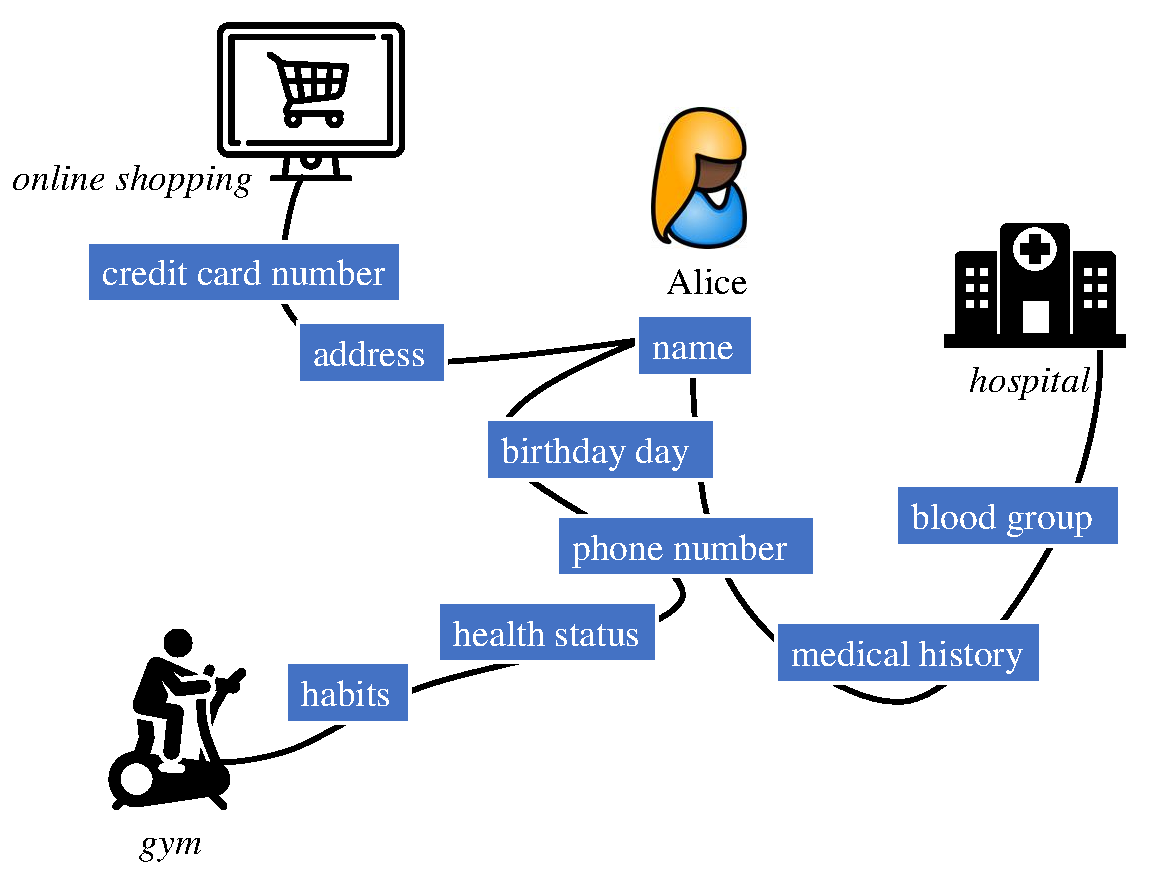
\includegraphics[width = 0.8\textwidth]{1-1}
\caption{Alice在不同场景下出示的属性信息}
\end{figure}

传统的凭证由于直接将属性信息与真实身份相关联,这样做会给Alice带来许多安全隐患。
比如Alice在去医院看病的过程中,医院就会得知Alice的血型、年龄及过往病史等一系列的信息。
这些信息都是直接跟Alice的身份挂钩,且大部分都是属于隐私的内容。
假如医院的数据库遭到攻击或医院直接出售这些信息,用户的个人信息安全将会面临巨大的威胁。

基于属性的凭证的作用是切断用户的属性与用户真实身份的关联,这种性质也被称为不可关联性(Unlinkability)。
因此在获取凭证的时候,用户需要的是获取对某个属性的凭证;在验证的过程中,用户只需提供必要属性的凭证即可,并且在整个验证的过程中,用户始终保持着匿名的状态。

\section{发展历程}[History]

基于属性的凭证的概念是从匿名凭证发展而来,而匿名凭证的思想最早是由Chaum\cite{chaum1985security}于1985年提出的,他主要围绕着如何在匿名的情况下完成交易提出了自己的一系列设想。
在这之后,Chaum与Evertse于1986年提出了一个解决方案\cite{chaum1986secure},这个方案需要有一个半诚实的(Semi-Honest)第三方机构\cite{张严2012匿名凭证方案研究进展,camenisch2001efficient},所谓的半诚实机构意味着它可以按照规则执行协议,也不会篡改执行的数据,但可以分析这些数据。这个方案由于可行性比较差,离实际应用还有一定距离。
经历了十多年的探索,同时也随着对数字签名,零知识证明等研究的不断深入,Camenisch和Lysyanskaya于2001年正式提出了第一个可行的匿名凭证方案\cite{camenisch2001efficient},这也是匿名凭证的概念第一次出现并被正式定义。
这个方案实现了包括假名生成,凭证的生成及凭证的展示等完整的协议,同时他们也对该方案的不可伪造性,匿名性,不可关联性及可行性等基本特性给出了完整的证明。
另外,他们在此基础上设计了一个扩展方案,这个扩展版的方案还满足了凭证不可出借及可撤销等与实际应用场景相关的特性。
作为第一个可行方案,此方案的安全性是基于强RSA假设和离散对数假设。

这个方案在构造上很大程度上受到假名系统(Pseudonym System)\cite{chen1996access,lysyanskaya1999pseudonym}的影响,也就是说,用户在请求凭证之前,需要从凭证发行者处获取假名,然后再使用假名的方式进行交互。
自第一个可行方案出现以后,关于匿名凭证的研究开始迈入新的篇章。
紧接着在2002年,Camenisch与Herreweghen给出了这一方案的具体实现,也就是Idemix系统\cite{camenisch2002design}。
同一时期,Brands基于盲签名的方法提出了一些有关匿名验证的思想\cite{brands1999rethinking},并在创建了Credentica公司之后基于此思想构建了一个匿名凭证系统U-Prove。
该系统随着2008年Credentica公司被微软收购由微软继续进行研发\cite{paquin2011u},已经成为最具代表性的匿名凭证系统之一。

匿名凭证系统的核心部分很大程度上依赖于数字签名,2001年的匿名凭证方案主要使用传统的RSA签名方案。
由于双线性映射的出现推动了数字签名的发展,伴随着许多基于双线性映射的签名方案的出现\cite{boneh2001short,camenisch2004signature,okamoto2006efficient},一些新的匿名凭证的方案构造也涌现出来。
基于双线性对的数字签名构造一般比较简洁,而且在同等安全条件下,签名长度相对RSA来说要短得多,如果用于匿名凭证的构造中会大大提高整个系统的效率。

2004年Camenisch和Lysyanskaya设计了一个基于双线性对的签名方案,并基于此签名方案提出了一个匿名凭证方案\cite{camenisch2004signature}。
在这个签名方案中,签名者可以在不知道签名内容$m$的情况下完成对$m$的签名。
更准确的说,签名者只知道$m$的承诺值$m'=\mathsf{Com}(m,r)$的情况下,生成对$m$的合法签名$\sigma$。
由于承诺机制满足隐藏和绑定这两个性质,在没有公开$r$的情况下,签名者无法获知所需签名的内容。
因此,这种签名方案能够用在匿名凭证系统的发行凭证这一过程中。
Camenisch和Lysyanskaya粗略地描述了利用此签名方案来构造匿名凭证系统的思路,构造出来的匿名凭证方案也没有提供可追踪性。
另一个基于此签名方案的是Blanton于2008年构造的一个匿名访问系统\cite{blanton2008online}。
这个系统可以看做匿名凭证系统的特殊情况,即把凭证发行机构与验证者合并起来看做一个服务提供商。
用户可以匿名地从服务商订阅服务,并以匿名的方式通过验证。
同年,Akagi,Manabe和Okamoto基于Okamoto提出的签名方案\cite{okamoto2006efficient}构造了一个包含完整的撤销机制的匿名凭证系统\cite{akagi2008efficient}。

由于普通的数字签名机制只能保证信息的完整性,并不能确保用户身份的匿名性。
因此在以上提到的匿名凭证系统中,为了保证匿名性,还使用了大量的零知识证明。
但是零知识证明需要多次的交互,且随着需要证明的内容增加,证明就变得越繁杂,这样就限制了匿名凭证系统的效率。
尽管我们可以使用Fiat-Shamir协议\cite{fiat1986prove}把一个交互式的零知识证明转换成一个非交互式的零知识证明,但是这种简单的转换无法用在双线性映射上\cite{张严2012匿名凭证方案研究进展},而且在安全性上需要基于随机预言机(Random Oracle)模型。

2008年,针对双线性映射上的非交互式零知识证明协议\cite{groth2008efficient}由Groth和Sahai提出,这种零知识证明协议(GS-Proof)具有一般性,因此能够很容易地应用到其他方案构造中。
自此之后,基于GS-Proof的匿名凭证系统方案也相继被提出\cite{belenkiy2008p,belenkiy2009randomizable}。
非交互式的证明方式为匿名凭证方案的构造带来了便利,更丰富了匿名凭证的应用场景。

在匿名凭证中比较重要的部分是对属性的签名,基于属性的凭证更能体现对属性的签名这一点。
自2012年之后,基于属性的凭证的概念开始替代了之前匿名凭证的称谓\cite{sabouri2012attribute},比如ABC4Trust这个项目中的ABC就是基于属性的凭证的英文缩写。
现在对基于属性的凭证的研究变得越来越细致,大多是针对特定的场景下设计可行的协议或针对某一个具体的性质进行改进。
比如有利用累加器(Accumulator)的方法来实现凭证撤销问题\cite{camenisch2009accumulator},或构建一个去中心化的基于属性的凭证系统\cite{garman2014decentralized},或利用结构保护的签名(Structure-Preserving Signature)来构造长度固定的凭证\cite{fuchsbauer2018structure},等等。

\section{基本结构及性质}[Construction]

在前面的介绍中,我们知道数字签名和零知识证明在基于属性的凭证方案的构造上起到了很关键的作用。
一般来说,凭证系统中的主要参与者可以分为用户(Users),凭证发行机构(Issuer)及验证者(Verifiers)这三类。
用户拥有者许多的属性,他们可以通过向凭证发行机构发起请求,以获取相关的属性凭证。
在获得相应的凭证之后,就可以通过匿名的方式提供相应的凭证给验证者,当通过验证后,用户就可以拥有获取相关服务的权限。
因此验证者有时也被称做服务提供者(Service Providers),三者之间的交互过程如图3-2所示。

\begin{figure}[h]
\centering
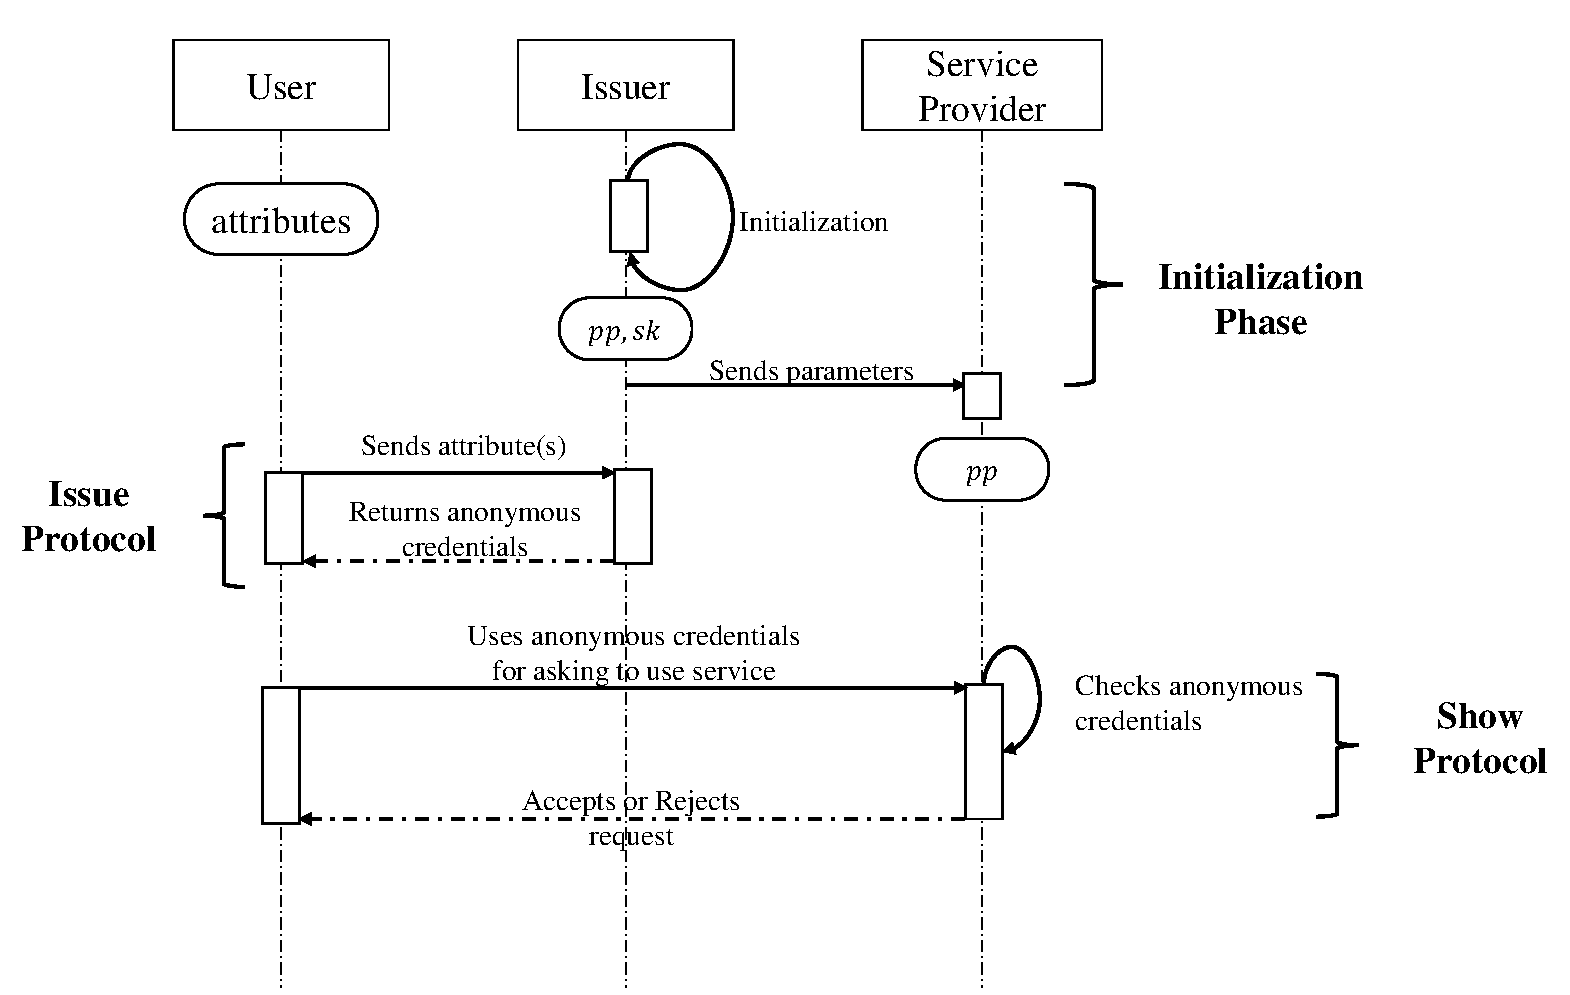
\includegraphics[width = 1\textwidth]{1-2}
\caption{基于属性的凭证系统中各角色交互的序列图}
\end{figure}

为了方便说明,下面我们分别用$\mathcal{U}$、$\mathcal{I}$和$\mathcal{V}$来表示用户,发行机构和验证者。
从图中我们可以看出,在一个基于属性的凭证系统中,主要包含初始化,发行凭证和使用凭证这三个阶段。
而要构造这样一个系统,关键在于如何实现发行凭证和出示凭证这两个协议。
初始化的过程一般是由$\mathcal{I}$来完成,一般在输入安全参数$\kappa$之后,得到系统输出的公共参数$pp$及私钥$sk$。
$\mathcal{I}$需要把$sk$保管起来,并将$pp$直接公开。$pp$一般包含系统的公钥及一些必要的参数,如在基于双线性映射的方案中,$pp$就包含$\mathbb{G}_1$,$\mathbb{G}_T$等信息。
$\mathcal{U}$在请求凭证之前,需要将自己的属性信息发送给$\mathcal{I}$。
当这些属性通过验证之后,$\mathcal{I}$可以使用$sk$对属性进行签名,并返回相应的基于属性的凭证。
在一些特殊情况下,$\mathcal{U}$不是直接把属性信息传递给$\mathcal{I}$,而是利用承诺机制对属性或一部分属性信息进行承诺,并将承诺结果发送给$\mathcal{I}$。
$\mathcal{U}$就可以利用这个凭证完成对属性的证明,$\mathcal{V}$利用之前收到的$pp$,就可以对凭证的真实性进行验证。
为了确保$\mathcal{U}$的身份不被泄漏,这里一般使用零知识证明的方式完成整个验证过程。

由此可知,在一个基于属性的凭证系统中,需要满足两个基本的性质,即可验证性(Authenticity)和匿名性(Anonymity)。

\begin{itemize}
  \item 可验证性:用户只有在拥有合法的凭证的情况下才能通过$\mathcal{V}$的验证。合法的凭证指的是此凭证是由$\mathcal{U}$从$\mathcal{I}$处获取且凭证没有被撤销。
  从另一个角度来说,满足可验证性即表示也满足不可伪造性,即用户$\mathcal{U}$不能伪造出一个合法的凭证。可验证性是由$\mathcal{I}$所使用的签名算法保证的。
  \item 匿名性:也可以称为身份与属性的不可关联性,即在$\mathcal{V}$通过$\mathcal{U}$的验证后,$\mathcal{V}$除了知道$\mathcal{U}$拥有相应的属性信息之外,并不能知道用户的真实身份。这主要是利用零知识证明的方式来实现的,通过这种方式可以充分地保护用户隐私。
\end{itemize}

除了这两个基本的性质外,针对现实生活中的场景,我们往往还需要考虑下面这几个性质:

\begin{itemize}
  \item 凭证的不可关联性:$\mathcal{U}$使用不同的凭证与$\mathcal{V}$交互,对于$\mathcal{V}$来说,不能判断出这多个凭证来自同一个用户。
  \item 可追踪性: 可追踪性指的是在必要的情况下,凭证的使用者是可以被还原出来的。因此如果满足了可追踪性,那也意味着此凭证不是绝对匿名的。
  执行追踪的一般是凭证发行机构$\mathcal{I}$或一个可信的第三方组织$\mathcal{O}$。此外,$\mathcal{O}$还需要满足不能伪造凭证这一性质。
  \item 可撤销性: 撤销一般是在凭证到期了或凭证被恶意使用的情况下执行的。要实现可撤销性,一般需要先实现可追踪性。在实际的应用场景中,可撤销还是一个很必要的特性。
\end{itemize}

\section{相关实例}[Application]

在这一节我们主要介绍已有的匿名凭证实例,这些实例包括IdeMix、U-Prove和ABC4Trust。

\subsection{IdeMix}[idemix]

IdeMix\cite{camenisch2002design}是第一个完整地实现了凭证的签发协议,使用协议并且支持撤销的匿名凭证系统,它是由Camenisch和Herreweghen在2002年设计出来的。
理论上主要基于Camenisch与Lysyanskaya在2001年提出的第一个匿名凭证方案\cite{camenisch2001efficient},这个方案使用的是RSA密码体制,安全性依赖于大整数分解的困难性。

在这个系统中,主要的参与者还是用户$\mathcal{U}$,凭证发行机构$\mathcal{I}$和验证者$\mathcal{V}$。
其中包含两个基本协议,即生成协议(Generation Protocol)与出示协议(Show Protocol),这两个基本协议中又包含了许多子协议。

\begin{itemize}
  \item[1.] \textbf{生成协议:}主要包含假名生成协议与凭证生成协议。$\mathcal{U}$通过向$\mathcal{I}$发送请求,以获取假名。
  然后用户就可以使用假名从$\mathcal{I}$处获取相应的凭证。
  \item[2.] \textbf{出示协议:}此协议主要是$\mathcal{U}$向$\mathcal{V}$证明自己拥有某个凭证,从而获取使用$\mathcal{V}$所提供的服务的权限。
\end{itemize}

在匿名凭证系统中,拥有一个可信的$\mathcal{I}$是很重要的,因为$\mathcal{I}$会保存着用户假名与凭证的对应关系。
因此,用户在与$\mathcal{I}$请求凭证的时候,可以每次选择不同的假名,这样能避免凭证与真实身份之间的关联。
$\mathcal{V}$作为服务提供者,可以看作一个提供在线视频的网站,或一个在线购物商城。
利用此系统,用户就可以用匿名的形式获取相关在线服务。
IdeMix系统不仅可以支持线上的服务,也可以支持离线的服务,如在智能卡上的应用\cite{bichsel2009anonymous}。

\subsection{U-Prove}[uprove]

U-Prove是微软公司开发的匿名凭证系统,它主要基于公钥密码学,椭圆曲线和哈希函数。
系统中也存在用户$\mathcal{U}$,凭证发行者$\mathcal{I}$以及验证者$\mathcal{V}$这三类角色。
与IdeMix类似,U-Prove中也包含生成和出示这两个基本的协议,但细节有所不同。

\begin{itemize}
  \item[1.] \textbf{生成协议:} $\mathcal{U}$从$\mathcal{V}$处获取一个token。
  \item[2.] \textbf{出示协议:} $\mathcal{U}$使用token通过$\mathcal{V}$的验证。
\end{itemize}

这里的token就包含了用户的属性信息。
通过使用一些密码学的方法,可以保证token不被篡改。
在U-Porve中,发行者$\mathcal{I}$使用的是盲签名的方式,用户$\mathcal{U}$则采取零知识证明的方式与$\mathcal{V}$进行交互。
此系统很好地保证了token与用户身份的不可关联性,但是如果多次使用同一个token则会破坏此不可关联性。
因此用户在每次验证前都需要使用一个新的token,只有这样才能确保完全的不可关联。

\subsection{ABC4Trust}[abc]

\begin{figure}[h]
\centering
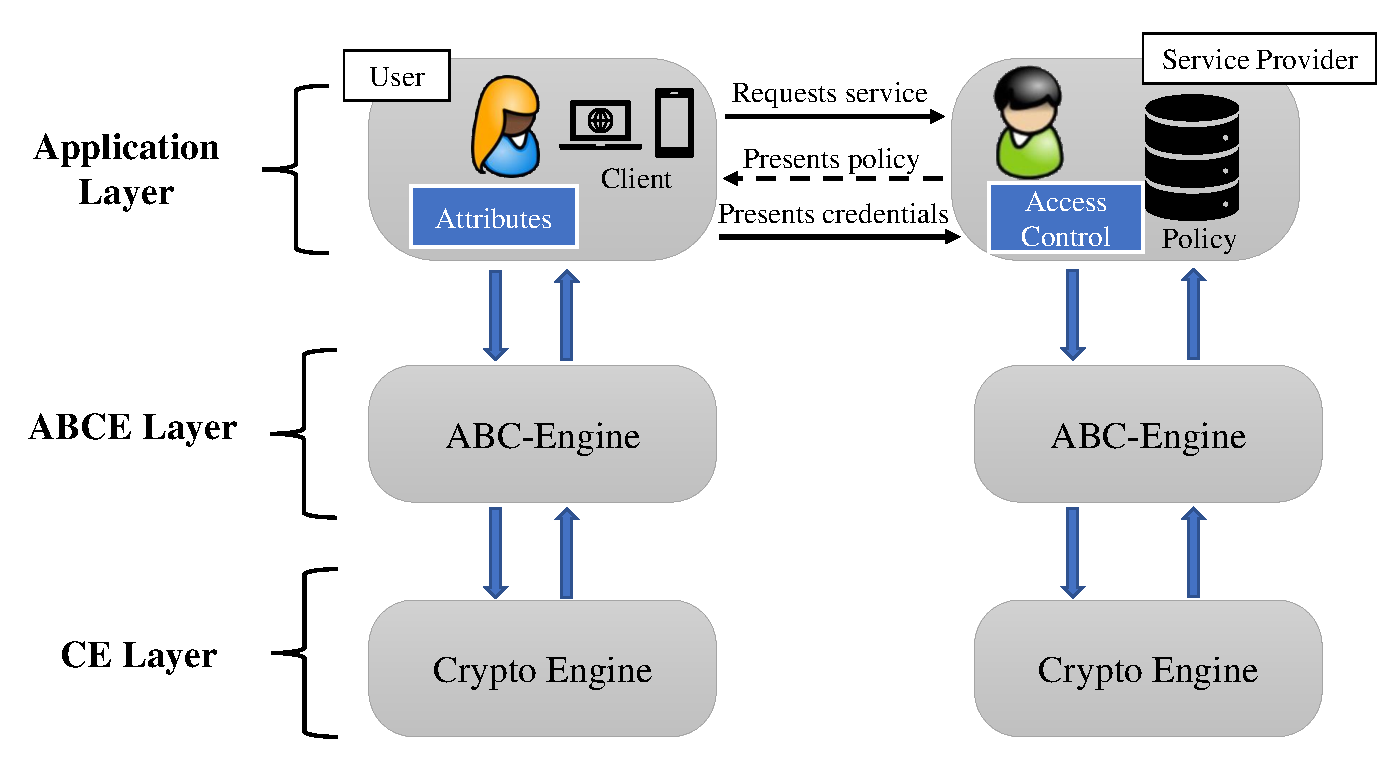
\includegraphics[width = 0.9\textwidth]{1-3}
\caption{ABC4Trust的基本结构}
\end{figure}

ABC4Trust,全称为Attribute-Based Credential for Trust,它是由欧盟资助的用来保护个人隐私的项目\cite{sabouri2012attribute}。
与前两个项目不同,ABC4Trust不仅关注在协议的设计,更多的是为基于属性的系统构建了一个完整的开发框架。
此项目为构建基于属性的凭证系统提供了一个完整的框架,它把用户$\mathcal{U}$与验证者$\mathcal{V}$之间交互的过程分成了三层,从上到下分别是应用层,ABC-Engine层和Crypto-Engine层。

正因为这种划分,我们可以在底层使用不同的密码学协议,层与层之间只需要提供相应的API接口即可。
ABC4Trust为基于属性的凭证系统的构造提供了一个比较规范的框架,这大大方便了开发者的对此类凭证系统的开发。

\section{本章小结}[Summary III]

在这一章,我们首先介绍了基于属性的凭证的发展历程,重点描述匿名凭证系统发展的几个阶段以及不同阶段的研究内容。
然后我们介绍了基于属性的凭证系统的基本结构及其需要满足的一些性质。
最后通过描述IdeMix,U-Prove和ABC4Trust这三个比较有代表性的现实生活中的实例,来说明匿名凭证系统的发展趋势。
其中IdeMix深受假名系统的影响,U-Prove利用了数字签名、承诺机制与零知识证明等方案,也是现在构建一个匿名凭证系统的常见做法。
ABC4Trust则着重于框架的设计,意在实现一套基于属性的凭证的标准。
通过对这几个实例的探讨,我们可以发现,随着对匿名凭证系统研究的深入,在构造方面逐步趋于规范化。
近年来,基于属性的凭证系统逐渐走向人们的生活中,在医疗、电子货币、电子身份证及物联网等方面都开始有了实际的应用\cite{neven2017privacy,viejo2019secure,de2018attribute}。
% !Mode:: "TeX:UTF-8"

% !TEX root = ../main.tex

\chapter{基于属性的凭证在车辆自组网中的应用}[Application in VANETs]

在前面的章节中,我们主要介绍了基于属性的凭证的相关概念,以及在保护个人隐私方面所发挥的作用。
现实生活中有很多需要身份验证的场景,大多数的场景都缺少一种保护用户隐私的措施,这会给用户本身带来很大的安全隐患。
如何在确保通过验证的同时又不泄露个人的隐私信息,这已成为隐私保护领域关注的热点问题之一。
车辆自组网环境就属于这类场景。

\section{车辆自组网}[Enviroment]

车辆自组网作为智能交通系统的重要组成单元,主要是为了解决道路安全问题以及为驾乘人员提供便利而出现的。
与现在热门的无人驾驶有很大不同,车辆自组网更侧重于提供辅助驾驶,主要集中在对车辆间通信的研究。
这个概念很大程度上来源于物联网,因此车辆自组网可以看做是实现车联网的一个必要组件。

车与车之间通过频繁的信息交换,可以用来实现智能化的交通系统。
想象在车辆自组网的环境中,我们可以通过接收其他车辆发送过来的信息,判断前面道路的拥挤状况,然后就可以挑选出最优的驾驶路线。
在一些比较复杂的路况下,我们还可以通过获取附近车辆的速度与它们的位置等信息,在判断可能出现危险的情况下,及时发出警告或者车辆主动采取紧急制动措施,这样就能避免许多交通事故的发生。
从这种角度来看,车辆自组网与无人驾驶是相辅相成的关系,如果能很好地实现车辆自组网,那么也将会推动无人驾驶的发展。

在车辆自组网的环境中,每辆车都要求配备一个称为车载通信单元(On-Board Unit,OBU)的设备。
这些设备可以将车辆的速度,位置及当前的路况等信息进行广播。
道路两旁会设置一些路边单元(Road-Side Units,RSUs),这些路边单元与交通管理中心(Transportation Regulation Center,TRC)相互联通,它们也可以与车辆进行通信,以提供交通服务等信息。

因此,我们可以把车辆自组网中的通信方式粗略分为两类,一类是车辆与车辆之间的通信,即V2V(Vehicle to Vehicle);另一类是车辆与RSUs这类的基础设施之间的通信,即V2I(Vehicle to Infrastructure)。
整个车辆自组网中的环境如图4-1所示。
目前的车辆自组网通信还没有形成统一的标准,比较有影响力的有基于DSRC(Dedicated Short Range Communications)技术的IEEE802.11p标准和基于LTE蜂窝网络的LTE-V标准。
以IEEE802.11p标准为例,它是在IEEE802.11的基础上专门针对车用通信网络改良的。
IEEE802.11p标准利用DSRC技术完成V2V和V2I两种通信方式。
DSRC是一种国际上通用的专门适用于车辆通信的技术,最早是由美国材料与实验协会于1992年提出,现在被广泛应用于电子不停车收费系统(Electronic Toll Collection,ETC)中。DSRC拥有延迟低、兼容性强等特点,已获得大多数车辆企业的支持。
DSRC技术要求车辆以一定的时间间隔(100到300毫秒)周期性地广播与交通相关的信息\cite{zhang2008raise}。
因此如何保证这些信息是可被验证的,这已经成为车辆自组网中需要关注的首要问题。

\begin{figure}[h]
\centering
\includegraphics[width = 0.9\textwidth]{V2X_v3_1}
\caption{车辆自组网的环境}
\end{figure}

正因为车辆自组网处于一种公开的环境中,所以很容易受到恶意的攻击。
如果恶意的车辆广播一些虚假的交通事故或交通堵塞信息,将会给其他车辆造成误导,从而破坏交通系统的秩序。
为了保障整个交通系统的安全,最简单的方法就是强制在广播的信息中附加可验证的车辆信息(如数字签名)。
这种做法提高了传播恶意信息的代价,虽然能确保整个交通系统的安全,但同时也在一定程度上泄漏了车辆的隐私。
% 给个引文 或者举个例子
现在的车联网通信标准首要考虑的是如何确保道路的安全,比如DSRC技术提供了ECDSA数字签名算法来保证信息的可验证性\cite{zhang2008raise}。
一些工作\cite{da2012examining,zhang2008raise}指出这种仅使用数字签名的方式会给车辆的隐私带来一定的风险。

隐私和安全是车辆自组网中重点关注的议题,隐私注重的是车辆的身份等信息不能完全暴露,而安全通常指的是交通系统的安全,它意味着车辆广播的信息是要能被认证。
欲保护用户的隐私,那么车辆在与其它车辆或RSUs进行通信的时候,需要保持一种匿名的状态。
但如果是完全匿名的话,一些恶意的车辆就会肆无忌惮地广播虚假的信息,这样会给整个交通系统带来不好的影响。
另外,在出现一些意外情况(如交通事故)时,我们还需要能够还原出信息签名者的真实身份。
因此在车辆自组网中,在满足可验证性的前提下,还需要满足匿名性及可追踪性。
从这些角度来看,我们会发现车辆自组网的环境与基于属性的凭证系统有许多相似的地方。

\begin{table}[htbp]
\bicaption[table1]{}{基于属性的凭证系统与车辆自组网环境的比较}
\vspace{0.5em}\centering\wuhao
\begin{tabular}{ccccc}
\toprule[1.5pt]
 & 基于属性的凭证系统 & 车辆自组网环境 \\
\midrule[1pt]
 需要认证的内容 & 用户的属性信息 & 车辆的速度,路况等信息 \\
 需满足的基本性质 & 可验证性,匿名性 & 可验证性,匿名性,可追踪性,实时性 \\
 可以信任的实体 & 凭证发行机构 & 交通管理中心 \\ 
\bottomrule[1.5pt]
\end{tabular}
\end{table}

通过表4-1,我们可以发现车辆自组网的环境与基于属性的凭证系统有着很多相似的地方。
除此之外,实时性是车辆自组网环境中必须要满足的一个性质,尤其是当车辆密度比较大或车辆处于高速移动的状态,实时性就显得尤其重要。
如果直接把现有的基于属性的凭证系统移植到车辆自组网系统中,则会因为无法保证实时性的要求而不可行。
如何设计出一个针对车辆自组网场景的方案,既能确保交通系统的安全和车辆的隐私,又能满足在特定场景中能还原用户的真实身份的需求,还能确保整个过程的高效性,是现在面临的主要问题。

\section{相关工作}[Related Schemes]

在车辆自组网研究的早期阶段,大多数的研究工作是围绕着如何确保信息的可验证性。
因此很自然地就有了使用数字签名的方法来防止信息的伪造\cite{el2002security}。
但这种方案显然会暴露隐私,因为用来验证信息的公钥可以对应看做车辆的身份信息\cite{petit2015pseudonym,da2012examining}。
近些年的研究工作开始集中在隐私保护方面,这些工作大多是基于假名的方式。

根据假名表示的方法不同,这些方案大致分为四类\cite{petit2015pseudonym}:
第一类是基于传统的公钥密码学,第二类是使用基于身份的密码学。
严格来说这两种方案都是公钥密码体制,核心思想都是用户自己申请多个公钥,然后通过频繁更换公钥的方式来维持匿名的状态。
在这里,假名可以看做是由公钥来表示的。
每个公钥会限制使用日期或使用次数,从而切断了公钥与真实身份之间的关联性。
前者是基于公钥基础设施(Public Key Infrastructure,PKI),因此需要使用公钥证书对车辆的公钥进行管理。
后者采用基于身份的密码学,由于不需要使用公钥证书,从而简化了公钥签发的过程。

然而,这种依赖频繁地更换假名保证匿名的方法并不能完全地阻止对身份的追踪\cite{wiedersheim2010privacy}。
因此许多工作开始关注如何更换假名,出现了像Mix-Context-Based、Mix-Zone-Based\cite{jemaa2017study,ying2013dynamic,lu2012pseudonym}等更换假名的策略。
但是这些策略都存在一定的局限性,并不能从根本上解决问题。

第三类方案是基于群签名的,这种方案的好处是不用考虑假名更换的问题。
群签名中存在着一个群管理员,群管理员可以添加或移除群成员,然后群成员可以使用自己的私钥对信息生成一个群签名。
群成员在验证签名的时候使用的是群公钥,因此能很好地满足匿名的特性,符合车辆自组网中对可验证性及匿名性的要求。
但群签名最大的弊端在于群管理员的权力过大,群管理员可以根据签名信息直接获取签名者的身份。
因此,有些方案提出使用RSUs作为群管理员\cite{hao2011distributed,park2011rsu},但由于RSUs长期处于公共环境中,很容易遭到攻击与破坏。
将RSUs作为群管理员,在实际中会给车辆的身份信息带来一定的风险。

第四类方案是基于对称密码学,这类方案是使用消息验证码来保障信息的完整性\cite{petit2015pseudonym,choi2005balancing}。
与公钥密码学最大的不同之处在于,对称密码学中签名与认证使用的密钥是相同的。
虽然此类方案的计算效率比较高,但由于使用的密钥是相同的,因此很难实现可追踪性。
大部分的方案都要求使用RSUs完成信息的验证与转发,系统的安全会严重依赖于RSUs。
而且由于RSUs的计算及存储能力有限,可能会成为整个车辆自组网的性能瓶颈。

与群签名类似的还有基于环签名的方案\cite{xiong2010efficient,chaurasia2011conditional,zeng2015privacy},相比基于群签名的方案,环签名中因为没有群管理员的存在,相对来说更加安全。
在这些方案中,车辆可以自由地生成签名,而不用依赖群管理员。
由于环签名本身是一种完全匿名的签名方案,为了满足车辆的可追踪性,需要在环签名的方案上进行一些改进,将这种完全匿名变为有条件的匿名\cite{张建明2012车辆自组网的位置隐私保护技术研究}。
正因为没有了群管理员的控制,车辆可以自发产生一个基于某个环上的签名。
但同时由于这种不可控制性,车辆自发生成的签名很可能是无效的。
现有的基于环签名的方案都没有讨论如何确保环成员的有效性,因为缺少适当的验证操作,车辆很容易会产生一个无效的签名,这会给整个交通系统带来不确定因素。

\section{构造方案}[Proposal Scheme]

通过前面的介绍,我们知道在车辆自组网中,车辆发送的消息一方面要能够被验证,另一方面要保证不泄漏隐私信息。
看上去与基于属性的凭证中对属性的要求很类似。但二者之间也存在着很明显的差别。

在基于属性的凭证系统中,消息的有效性是靠凭证发行机构的签名保证的;
而车辆自组网的环境中,车辆不能频繁地与TRC通信,因此信息的签名过程是由车辆自己完成的。
那么,我们可不可以直接使用一种具有匿名性质的签名体制来同时保证匿名性和可验证性呢?

考虑到车辆自组网的特殊结构,环签名看上去是很不错的解决方案。
但是环签名具备极高的自发性,如果车辆可以自由收集其他车辆的公钥并对消息进行签名的话,很容易由于环中存在失效的成员而使签名无效。
现有的基于环签名的方案\cite{xiong2010efficient,chaurasia2011conditional,zeng2015privacy}都没有考虑这个问题。
在这些方案中,为了突出环签名的优势,直接移除了RSUs,没有考虑V2I能发挥的作用。
那么我们为什么不能将RSUs放到基于环签名的方案中呢?
如果可以将RSUs融入进去,并使用V2I的方式分配环成员,是不是就可以解决这个问题呢?

因此我们希望将RSUs与基于环签名的方案结合。
在车辆进入某一区域时,需要通过向区域内的RSUs发出请求来获取一个成员列表。
RSUs在验证车辆的身份后,向其分配一个有效的成员列表。
车辆收到这个列表后,便可以使用环签名的方式对需要发送的信息进行签名。

虽然环签名可以同时满足可验证性和匿名性这两个基本性质,但环签名带来的匿名是无条件的。
因此我们需要在签名上面附加一些可追踪的信息。
以往的许多方案中,追踪这一功能是由TRC完成的,即TRC拥有权力可以直接根据生成的签名等信息还原出签名者的真实身份。
但在实际中并不完全是这样,想象在出现交通事故时,一般是需要有执法部门完成对信息源的追踪,TRC应该是起到辅助追踪的作用。
因此我们引入了执法机关(Law Enforcement)这样一个实体,利用这种机构完成签名的追踪,并解析出签名者的假名。
如果有进一步的需要,执法机关还可以根据这个假名从TRC的数据库中还原出其对应的真实ID,并进行撤销操作。

要合理使用密码学的工具来构建这样一个方案不是容易的事情,一方面我们需要避开以前方案的劣势,另一方面我们需要在效率上满足一定的要求。这就需要与其它方案进行对比,还要找到合适的衡量方法体现方案高效率的特点。另外,在说明我们方案满足的性质的时候,需要对满足的这些性质进行合理的论证,有必要的话还可以采取形式化的证明方式。
为了方便证明,我们也可以引入随机预言机模型。
在证明之前,通常需要引入合理的假设前提,并给出攻击者的攻击模型。

按照这样的思路,首先我们把车辆的假名按照从生成到撤销划分为六个阶段,每个阶段包括一些具体的操作过程,如图4-2所示。

\begin{figure}[h]
\centering
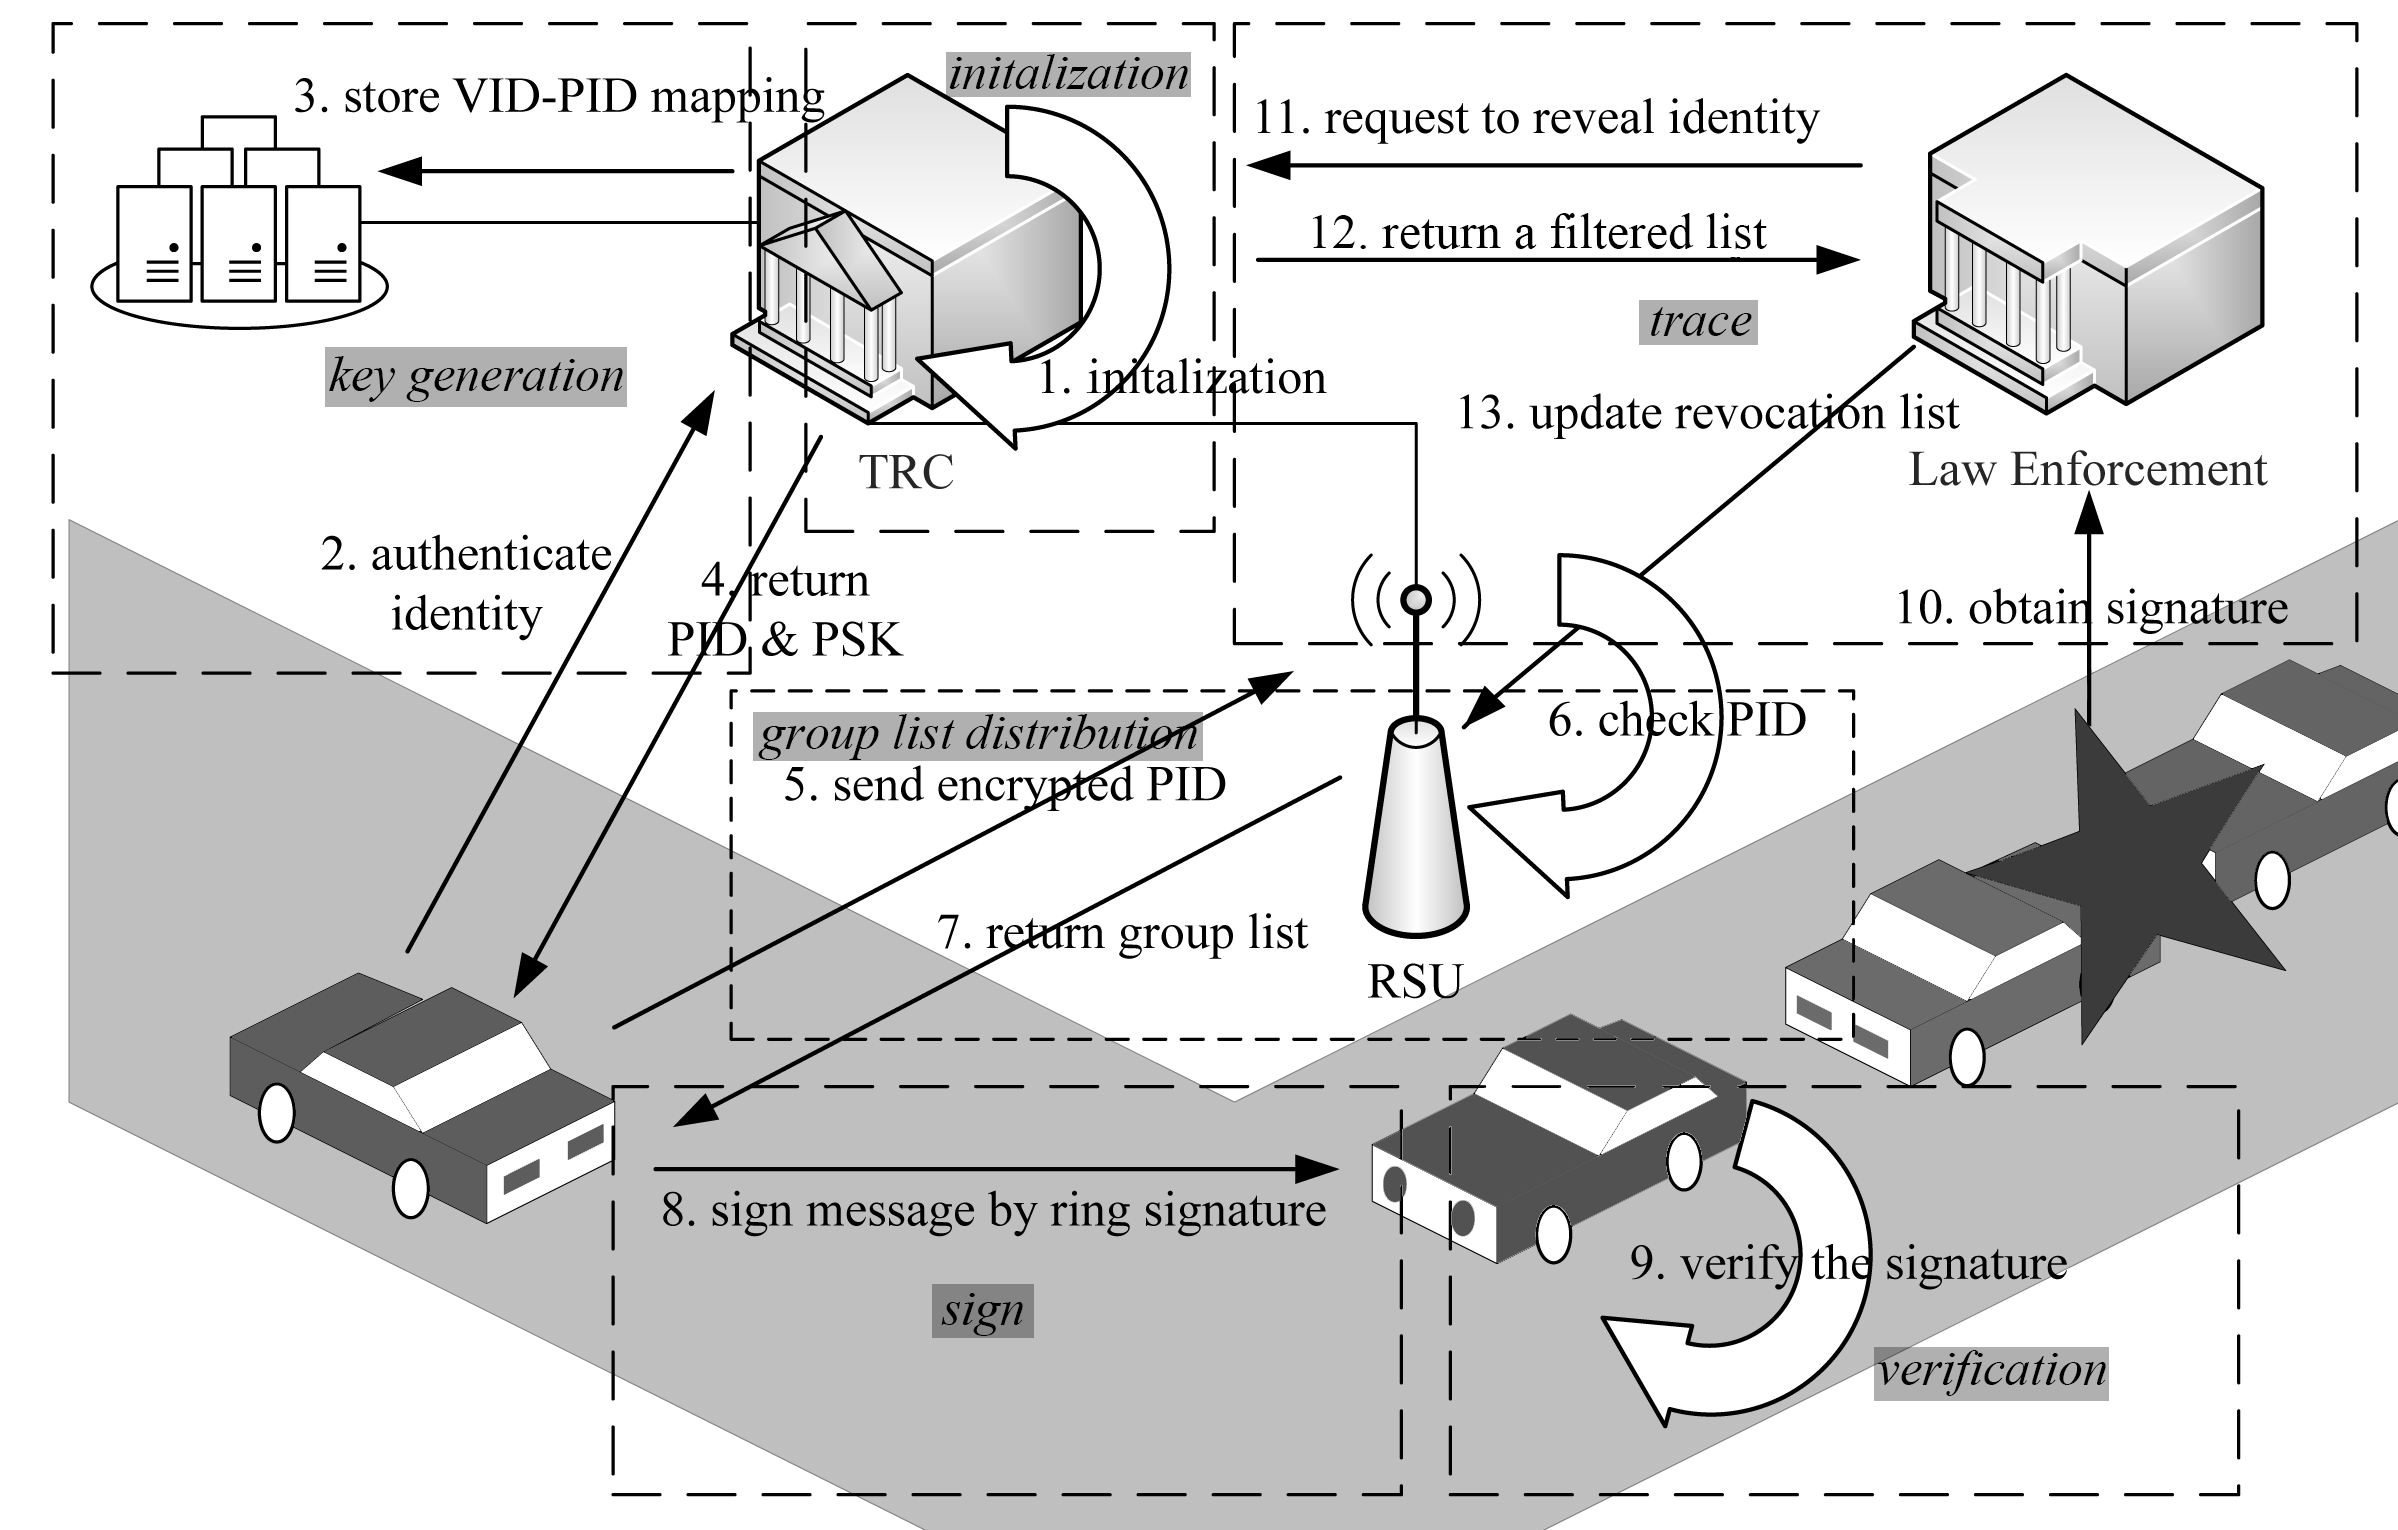
\includegraphics[width = 0.9\textwidth]{V2X_v6}
\caption{方案构造}
\end{figure}

从图中可以看到,在我们的方案中共有4类参与者,它们分别是交通管理中心(TRC),执法机关,配备了OBUs的车辆以及道路两旁的RSUs。
在充分考虑到RSUs特殊身份的情况下,我们提出使用基于身份的加密方案来完成车辆向RSUs的请求列表过程,利用对称密码机制完成RSUs的成员列表分配过程。

根据双线性映射的性质,保证在一次交互之后,双方可以获得相同的密钥信息。
为了完成追踪,我们在为签名的内容附加一个可追踪的$tag$。
为了方便说明,我们把需要使用的符号以及它所表示的含义列举出来,如表4-2所示。

\begin{table}[htbp]
\bicaption[table2]{}{符号及其含义}
\vspace{0.5em}\centering\wuhao
\begin{tabular}{ccccc}
\toprule[1.5pt]
 符号 & 含义 \\
\midrule[1pt]
 $s$ & TRC的主私钥 \\
 $PK$ & TRC的公钥\\
 $s_{trac}$ & 执法机关的私钥\\
 $PK_{trac}$ & 执法机关的公钥\\
 $PP$ & 公共参数\\
 $VID$ & OBUs的真实ID\\ 
 $PID$ & OBUs的公钥(也称作假名)\\
 $PSK$ & OBUs的私钥\\
 $RID$ & RSUs的公钥\\
 $RSK$ & RSUs的私钥\\
 $k_{i-j}$ & i 与 j 之间的共享公钥\\
 $L$ & 成员列表,用于环签名\\
 $t_d$ & $L$的失效时间\\
 $t$ & 签名的时间戳\\
 $tag$ & 用于追踪的标签\\
 $a||b$ & 将字符串$a$与$b$进行连接\\
\bottomrule[1.5pt]
\end{tabular}
\end{table}

每一个步骤的操作细节我们将按照初始化,密钥生成,成员列表分配,签名,验证和追踪这六个阶段分别进行介绍。

\subsection{初始化}[Setup]

系统的初始化过程包含一个$\mathsf{Setup}$算法,这个算法是由TRC执行的。
由于我们的方案是利用双线性映射来实现的,初始化的结果就是生成了一个双线性映射及相关的一些参数。
\begin{itemize}
  \item $(pp,s)\leftarrow\mathsf{Setup}(1^\kappa)$:在初始阶段,对于给定的安全参数$\kappa$,算法$\mathsf{Setup}(\cdot)$可以生成公共参数$pp$和TRC的私钥$s$。其中$s\in_R\mathbb{Z}^*_q$是随机选取的,$pp=(\mathbb{G}_1,\mathbb{G}_T,P,q,e,PK,H_1,H_2)$。
  $\mathbb{G}_1$与$\mathbb{G}_T$均为阶数为$q$的循环群,$e:\mathbb{G}_1\times\mathbb{G}_1\rightarrow\mathbb{G}_T$是一个双线性映射。
$P$是$\mathbb{G}_1$的一个生成元,$PK$又被称为TRC的公钥,且有$PK=s\cdot P$。
$H_1$和$H_2$是两个密码哈希函数,且$H_1:\{0,1\}^*\rightarrow\mathbb{G}_1$,$H_2:\{0,1\}^*\rightarrow\mathbb{Z}_q^*$。
\end{itemize}

在完成初始化过程之后,TRC可以将$pp$进行公开,并保管好私钥$s$。
为了实现可追踪性,执法机关需要根据初始化后的公开参数$pp$生成对应的密钥对$(s_{trac},PK_{trac})$。
其中$s_{trac}\in_R\mathbb{Z}_q^*$,为执法机关的私钥,在进行追踪时会用到;$PK_{trac}=s_{trac}\cdot P$,作为执法机关的公钥,可以事先载入到车辆的OBUs设备中。

\subsection{密钥生成}[Keygen]

在初始化完成之后,RSUs和配备有OBUs的车辆就可以从TRC处获取自己的密钥对。
在这里我们需要做一个假设,即每辆车的OBU中都存在一个硬件安全模块(Hardware Security Module,HSM)\cite{tzeng2017enhancing}。
存储在HSM中的信息不会遭到篡改,同时一些与密码学有关的操作如加密,签名等也是在HSM中完成。

系统中,每一辆车都有一个唯一的身份编号,我们用$VID$来表示。
对于真实身份为$VID_\ell$的车辆,它可以通过向TRC提交$VID_\ell$来获取自己的密钥对。
TRC在收到$VID_\ell$之后,开始执行$\mathsf{KeyGen}(VID_\ell)$算法,并把生成的密钥对及$pp$载入到HSM中。

\begin{itemize}
  \item $(PID_\ell,PSK_\ell)\leftarrow\mathsf{KeyGen}(VID_\ell)$:输出的$PID_\ell$和$PSK_\ell$分别代表着$VID_\ell$的公钥和私钥。
  其中$PID_\ell=H_1(VID_\ell||salt)$,$PSK_\ell=s\cdot PID_\ell$。$salt$是随机选取的,即$salt\in_R\mathbb{Z}_q^*$。
  为了实现可追踪性,执法机关的公钥$PK_{trac}$需要事先存储在HSM中。
  TRC还会把$PID_\ell$与$VID_\ell$对应起来保存在数据库中。
\end{itemize}

类似地,对于真实身份为$ID_j$的RSU来说,它获取到的密钥对为$(RID_j,RSK_j)$,其中$RID_j=H_1(ID_j)$,$RSK_j=s\cdot RID_j$。
与车辆编号$VID_\ell$不同,RSU的身份编号$ID_j$是可以直接公开的。
因此对于车辆而言,某一区域内的RSUs信息均为可查的。

这里RSUs与OBUs获取假名的方式略有不同,OBUs获取到的假名是在$VID$的基础上加盐哈希产生的,目的是车辆可以在不用更换$VID$的情况下可以从TRC处获取新的假名,满足车辆定期更换假名的需求。

由于RSUs是公共设施,而且IDs都是可以公开查询的,直接使用哈希获取假名的方式能够容易让其它车辆进行检验。
即当车辆进入某一区域时,由于事先知道这一区域RSUs的IDs,便可直接使用哈希函数$H_1$来计算RSUs的公钥(假名)。
这样就可以使用此公钥进行数据的加密,从而避免出现与伪装成RSUs的设备进行通信的情况。

\subsection{成员列表分配}[groupList]

当车辆进入一个区域时,它首先需要向该区域内的RSUs发送请求,在请求通过后,RSUs再向其发送一个成员列表。
为了方便说明,不妨假设车辆$VID_\ell$在与$RSU_j$进行通信,在这一过程中,我们使用第二章2.4节中的基于身份的加密方案,并使用$\mathsf{Enc}$和$\mathsf{Dec}$分别表示此方案的加密和解密算法\cite{boneh2001identity}。
另外,我们使用$\mathcal{ENC}(\cdot)$,$\mathcal{DEC}(\cdot)$,$\mathcal{HMAC}(\cdot)$分别表示对称密码体制下的加密算法、解密算法以及消息验证码算法。
具体的通信过程可以分为以下几个步骤:

\begin{itemize}
  \item $RSU_j$ 在该区域内广播自己的公钥$PID_j$;
  \item $VID_\ell$进入该区域后,首先可以获得$PID_j$。
  由于$ID_j$是公开的,因此$VID_\ell$可以直接用哈希算法判断$PID_j$的真实性。
  之后$VID_\ell$就可以使用$PID_j$加密自己的假名,即$C=\mathsf{Enc}(PID_\ell,RID_j)$,并把加密后的密文$C$发送给$RSU_j$;
  \item $RSU_j$在收到密文$C$之后后,可以利用自己的私钥计算出$VID_\ell$的公钥,即$PID_\ell=\mathsf{Dec}(C,RSK_j)$;
  \item $RSU_j$开始检验$PID_\ell$是否失效,如果已经失效,则直接拒绝$VID_\ell$的请求,并终止与$VID_\ell$的通信;
  \item 如果$PID_\ell$是合法的,$RSU_j$就可以计算共享密钥$k_{j-\ell}=e(PID_\ell,RSK_j)$,并使用此密钥来加密群成员信息;
  \item $RSU_j$选取一定的车辆公钥组成一个群成员列表$L$,并使用对称密码学中的Encrypt-then-MAC的方法来传递$L$,即先计算$C^*=\mathcal{ENC}_{k_{j-\ell}}(L)$,再计算$\Sigma=\mathcal{HMAC}_{k_{j-\ell}}(C^*||t_d)$,最后发送$(C^*,\Sigma,t_d)$给$VID_\ell$,其中$t_d$表示的是$L$的失效时间;
  \item $VID_\ell$在收到$RSU_j$发送的密文$C^*$后,首先计算它们之间的共享密钥$k_{\ell-j}=e(PSK_\ell,RID_j)$,在消息认证码$\Sigma$通过验证后便可以还原出成员列表$L=\mathcal{DEC}_{k_{i-j}}(C^*)$。
\end{itemize}

\subsection{签名}[sign]

在这里我们使用$\mathsf{Sign}$与$\mathsf{Verify}$分别表示前面介绍的基于身份的环签名的签名算法和验证算法。
这两个算法的具体构造见第二章2.4节。

在拿到成员列表$L$之后,$VID_\ell$便可以使用$L$来完成环签名。
对于$L=\{PID_1,PID_2,...,PID_n\}$ $(1\leq \ell\leq n)$,这个过程由车辆OBU中的HSM完成。首先HSM会生成一个当前的时间戳$t$,那么就可以计算可追踪的标签$tag$:
\begin{equation}
tag=e(H_1(VID_\ell||t),PK_{trac})
\end{equation}
然后$VID_\ell$可以使用第二章2.4节中介绍的环签名的方法生成对消息$m$的签名,即$\sigma=\mathsf{Sign}(m||t_d||tag||t,PSK_\ell,L)$,
最后$VID_\ell$广播$(m,\sigma,L,t_d,t,tag)$。

\subsection{验证}[verify]

当车辆$VID_k$收到$(m,\sigma,L,t_d,t,tag)$后,首先需要通过$t_d$判断$L$有没有失效。
如果没有失效,$VID_k$再执行验证算法$\mathsf{Verify}(m||t_d||tag||t,\sigma,L)$来验证$m$的有效性。

\subsection{追踪}[trace]

追踪是指当出现一些意外情况时,可以通过一些方法还原出签名者的真实身份。
在过去提出的一些方案中,追踪是由TRC完成的,TRC无疑拥有最高的权力。
但在我们的方案中,要完成签名的追踪需要TRC与执法机关共同完成。
追踪的过程主要依赖对$tag$中信息的分析。
假设执法机关获取了$tag=e(H_1(VID_\ell||t),PK_{trac})$后,首先它可以将$(L,t)$发送给TRC,TRC根据数据库中假名与车辆真实$VID$之间的对应关系找到相应的$VID_\ell$,也就是对于$1\leq i \leq n$,可以计算
\begin{equation}
H'_i=e(H_1(VID_i||t),P)
\end{equation}
并把结果$\{H'_1,H'_2,...,H'_n\}$返回给执法机关。

执法机关在收到$\{H'_1,H'_2,...,H'_n\}$之后,首先利用自己的私钥将$tag$还原,即:
$$tag'=tag^{1/s_{trac}}$$
然后对$\{H'_1,H'_2,...,H'_n\}$中的每个成员与$tag'$进行比较,从中找出与$tag'$相等的$H'$。
那么被定位到的即为真正的签名者,执法机关可以根据此信息获取到签名者的假名。
需要进一步说明的是,根据假名信息,执法机关可以向TRC进行请求获得对应的真实$VID$,如果该车辆需要被撤销,执法机关可以将其写入撤销列表。
更新的撤销列表会同步到RSUs中,那么在之后的验证过程中,RSUs将会直接拒绝该失效车辆的任何请求。

\section{比较与分析}[Comparison]

这一节主要是将我们的方案与其他方案进行对比分析。
之前提出的一些基于公钥密码学和使用基于身份的密码学的方案都存在着假名更换的问题,由于我们的方案使用的采取的是环签名的机制,可以很好地避开这个问题。
另外与其它环签名的方案相比,我们的方案能够很好地保障环成员列表可靠性。
近些年,有一些使用了防篡改设备(Tamper-Proof Devices)在本地生成假名的方案\cite{yang2019lightweight,tzeng2017enhancing,lee2013toward},我们在表4-3中列出了与这些方案的比较。

\begin{table}[htbp]
\bicaption[table1]{}{与其他方案的比较}
\vspace{0.5em}\centering\wuhao
\begin{tabular}{ccccc}
\toprule[1.5pt]
 & 我们的方案 & 方案I\cite{yang2019lightweight} & 方案II\cite{tzeng2017enhancing}  & 方案III\cite{lee2013toward} \\
\midrule[1pt]
 不可伪造性 & $\surd$ & $\surd$ & $\surd$ & $\surd$ \\
 可追踪 & $\surd$ & $\surd$ & $\surd$ & $\surd$ \\
 不可关联性 & $\surd$ & $\surd$ & $\surd$ & \text{\sffamily X} \\
 假名的可验证性 & $\surd$ & $\surd$ & \text{\sffamily X} & \text{\sffamily X}\\
 抗中间人攻击 & $\surd$ & $\surd$ & $\surd$ & $\surd$ \\
 抗重放攻击 & $\surd$ & $\surd$ & $\surd$ & $\surd$ \\
 假名(公钥)更换频率 & 低 & 高 & 高 & 高\\
 对RSU的要求 & 半诚实 & 完全信任 & 完全信任 & 完全信任 \\
 完成追踪的实体 & TRC与执法机关合作 & TRC & TRC & TRC \\
\bottomrule[1.5pt]
\end{tabular}
\end{table}

在对这些性质进行分析之前,我们先对车辆自组网中各个参与者建立如下的前提假设:

\begin{itemize}
  \item 在这个系统中,TRC与执法机关是完全可信的。由于TRC是整个系统的核心部分,车辆与RSU的密钥都是依赖它分配的。
  执法机关只有在需要追溯恶意的签名者时才会去向TRC发送追踪请求。并且我们假设他们之间不会共谋;
  \item RSUs在这个系统中可以看做不完全受信任的(Semi-Trusted),这意味着RSUs会正常执行系统的协议,但可能会尝试去分析车辆发送的信息。
  换句话说,RSUs在分配成员列表的过程中,不会去修改需要发送的信息,但可能通过分析车辆发送的信息尝试还原车辆的真实身份;
  \item 系统中的车辆可以修改通信的数据信息,但一些保存在HSM中的参数是不可修改的且不会外泄的。且在HSM中进行的操作我们都可以认为是安全的;
  \item 系统中的通信环境是不安全的,攻击者可以窃听并修改通信过程中的数据信息,或者直接伪造虚假信息来破坏系统的安全性。
\end{itemize}

对于硬件安全模块HSM,我们可以将其看做由5个不同功能的子模块组成,这5个模块分别为假名校验模块,加密模块,解密模块,签名模块和验证模块。这些模块可以通过一定的输入来得到相应的输出结果。这些模块的组成如图4-3所示。

\begin{figure}[h]
\centering
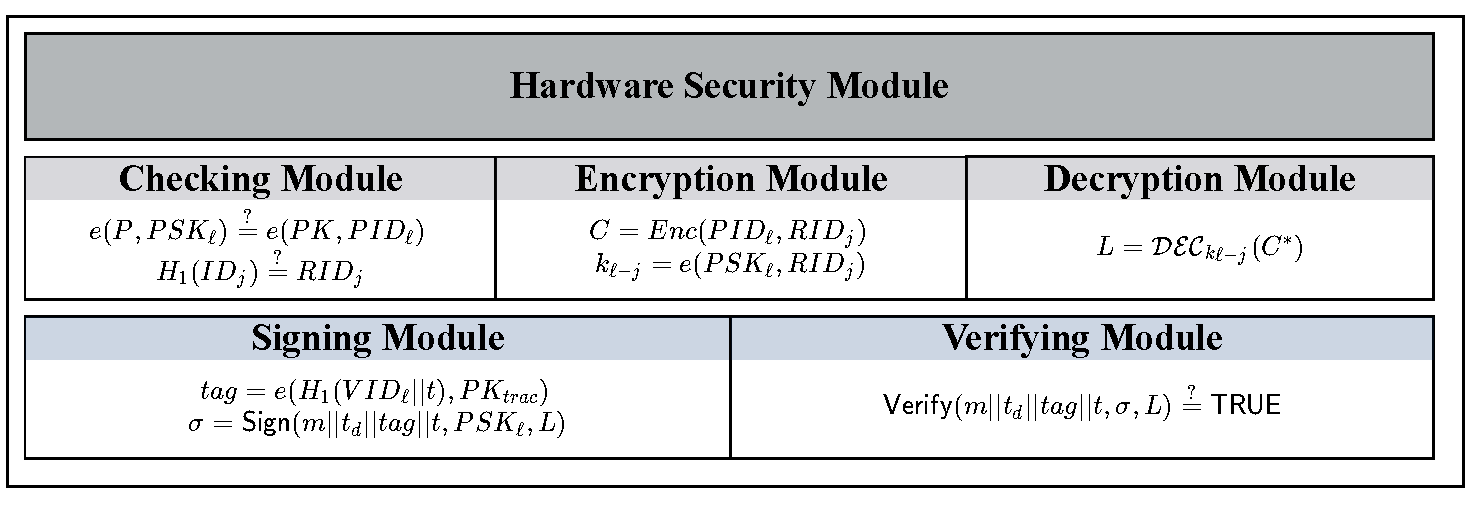
\includegraphics[width = 1.0\textwidth]{hsm}
\caption{组成HSM的各个模块}
\end{figure}

当TRC完成初始化工作之后,生成的公共参数$pp=(\mathbb{G}_1,\mathbb{G}_2,P,q,e,PK,H_1,H_2)$被预先载入到HSM模块中。从图中可以看出,当车辆$V_\ell$获取到自己的密钥对$(PID_\ell,PSK_\ell)$并将密钥对载入到HSM中时,HSM中的假名校验模块首先对这对密钥进行校验。

校验的过程就是检查以下等式是否成立:
\begin{equation}
e(P,PSK_\ell)\overset{?}{=}e(PK,PID_\ell)
\end{equation}
如果校验通过,那么HSM就可以载入这对密钥以进行后面的操作。

在成员列表分配阶段,车辆$V_\ell$在收到$RSU_j$的公钥$PID_j$之后,首先需要调用HSM的假名校验模块来校验$RSU_j$的公钥$PID_j$是否合法。
由于不同区域内的RSUs身份信息$ID_j$都是公开可查的,通过提供$PID_j$和$ID_j$给HSM,HSM只需要检查以下等式是否成立:
\begin{equation}
H_1(ID_j)\overset{?}{=}RID_j
\end{equation}
如果校验通过,HSM中的加密模块便自动使用$RID_j$作为加密的公钥对车辆的假名$PID_\ell$进行加密。即计算:
\begin{equation}
C=\mathsf{Enc}(PID_\ell,RID_j)=(rP,PID_\ell\oplus g_d^r)
\end{equation}
其中,$g_d^r=e(PID_\ell,PK)$。

在输入加密的密文之后,HSM还需要计算与$RSU_j$对应的共享密钥,即计算:
\begin{equation}
k_{\ell-j}=e(PSK_\ell,RID_j)
\end{equation}
并把此共享密钥作为解密模块的解密密钥。

在收到$RSU_j$返回的$(C^*,\Sigma,t_d)$之后,HSM的解密模块开始验证$t_d$是否失效,如果还未失效则再验证消息验证码$\Sigma$。在这些都通过验证之后,便可以使用对称解密算法$\mathcal{DEC}_{k_{\ell-j}}(C^*)$对密文$C^*$进行解密。
值得注意的是,在实际应用中,我们可以使用AES作为对称加解密算法,这类算法现在已经很成熟,计算效率比较高。

在完成了对成员列表的还原之后,签名模块便可以使用此列表$L$作为输入,并输出对消息$m$的一个环签名。
验证模块则是在收到其它车辆的签名信息后,利用验证算法$\mathsf{Verify}$完成对消息$m$的验证。

下面我们将对此方案满足的可验证性、匿名性、不可伪造性、可追踪性、抗重放攻击以及高效性分别进行说明。
为了方便描述,我们依然使用$V_\ell$代表进行签名的车辆,用$V_k$表示验证签名的车辆。

\subsection{可验证性}[authentication]

可验证性指的是,在此方案中如果所有过程都是正确执行的,那么最终得到的签名一定可以通过验证。
因此我们需要考虑成员列表分配过程以及签名和验证过程的正确性。
从前面的描述我们可以知道,$V_\ell$在向$RSU_j$请求成员列表时,发送给$RSU_j$的密文是:
\begin{equation}
C=(rP,V)=(rP,PID_\ell\oplus g_d^r)
\end{equation}
$RSU_j$在收到此密文后,计算$V\oplus e(RSK_j,rP)$,由于:
\begin{equation}
V\oplus e(RSK_j,rP)=V\oplus e(RID_j,s\cdot P)^r=V\oplus g_d^r=PID_\ell
\end{equation}
因此$RSU_j$能够正确获取车辆$V_\ell$的假名$PID_\ell$。
而$RSU_j$计算的共享秘钥为$k_{j-\ell}=e(PID_\ell,RSK_j)$,$VID_\ell$计算的共享秘钥为$k_{\ell-j}=e(PSK_\ell,RID_j)$,由双线性映射的性质可以得到:
\begin{equation}
e(PID_\ell,RSK_j)=e(PID_\ell,s\cdot RID_j)=e(s\cdot PID_\ell,RID_j)=e(PSK_\ell,RID_j)
\end{equation}
双方在这个交互过程中获取了相同的密钥,再根据对称密码体制的特点,从而保证$V_\ell$可以从$RSU_j$处正确获取成员列表信息。

对于车辆$V_\ell$以及成员列表$L=\{PID_1,PID_2,...,PID_n\}$ $(1\leq \ell\leq n)$,以及所需签名的信息$m$,我们可以令$m'=m||t_d||tag||t$。那么通过得到的签名$\sigma$为:
\begin{equation}
\sigma=(\cup_{i=1}^n\{U_i\},V)
\end{equation}
其中,对于$1\leq i\leq n$且$i\neq \ell$,$U_i$都是从$\mathbb{G}_1$中随机选取的,我们记$h_i=H_2(m'||L||U_i)$。计算完成后我们可以随机选取$r'_\ell \in_R\mathbb{Z}_q^*$,并计算$U_\ell=r'_\ell PID_\ell-\sum_{i\neq \ell}\{U_i+h_iPID_i\}$,$h_\ell=H_2(m'||L||U_\ell)$。最后可得到$V=(h_\ell+r'_\ell)PSK_\ell$。

在验证的过程中,对于$1\leq i \leq n$,车辆$V_k$首先计算$h_\ell=H_2(m'||L||U_i)$,那么根据双线性映射的性质,我们可以得到下面的等式:
\begin{equation}
\begin{split}
e(PK,\sum_{i=1}^n(U_i+h_iPID_i)) = & e(s\cdot P,U_\ell+h_\ell PID_\ell+\sum_{i=1,i\neq \ell}^n(U_i+h_iPID_i)) \\
 = & e(s\cdot P,r_\ell'PID_\ell+h_\ell PID_\ell)  \\
 = & e(s\cdot P,(r_\ell'+h_\ell)PID_\ell) \\
 = & e(P,(r_\ell'+h_\ell)PID_\ell\cdot s) \\
 = & e(P,V) \\
\end{split}
\end{equation}
因此,只要$V_\ell$正确执行相关的协议,那么产生的签名一定能够通过$V_k$的验证。

\subsection{匿名性}[anonymous]

我们主要从V2I和V2V两个角度分析匿名性,从V2I的角度,由于$RSU_j$是半诚实的,在与车辆$V_\ell$的通信过程中,它唯一知道的就是车辆$V_\ell$的公钥,即$PID_\ell$。
由于$PID_\ell$是由TRC生成的,且$PID_\ell=H_1(VID_\ell||salt)$。
根据密码哈希函数的单向性,在只知道$PID_\ell$的情况下,$RSU_j$能在概率概率多项式时间内找到一个$ID$使得$H_1(ID)=PID_\ell$的概率是可以忽略不计的。
而且我们建议车辆的公钥需要定时更新,由此保证了$RSU_j$无法将$PID_\ell$与车辆的真实身份关联起来。

从V2V的角度,由于我们选择的是由Chow,Yiu和Hui提出的基于身份的环签名方案,这种环签名方案具有完全的匿名性,因此在知道车辆$V_\ell$生成的签名$\sigma$的情况下,车辆$V_k$根据列表$L$只能推断出签名者在列表$L$内这条信息,并不能推断出签名者具体是列表中的哪一位。这样就能够很好地保证签名者的匿名性。
另外,在广播的信息中还存在可追踪的标签,即$tag=e(H_1(VID_\ell||t),PK_{trac})$。
密码哈希函数的性质保证了车辆$V_k$不能根据$tag$的值从中获取到有用的信息。

\subsection{不可伪造性}[non-repudiation]

在前面的假设中,我们假定RSUs是不完全受信任的,也就是说RSUs不会篡改或伪造数据,因此我们在考虑不可伪造性时,只需要考虑系统中的恶意车辆。
与前面分析类似,我们分别从V2I与V2V两个方面进行说明。

在V2I的过程中,假设有一恶意的车辆$VID_{i'}$想伪装成$VID_\ell$并与$RSU_j$进行通信。
假设$VID_{i'}$已经知道了$VID_\ell$的公钥为$PID_\ell$,那么$RSU_j$向他返回的就是用$k_{j-\ell}$加密的信息。
由于我们使用的是对称密码体制,并且采用Encrypt-then-MAC的模式。
这种模式是满足选择密文安全的,也就是说$V_{i'}$在没有密钥$k_{j-\ell}$的情况下不能获取到任何有用的信息。
因此我们只需要证明$V_{i'}$在只知道$PID_\ell$的情况下对它获取到密钥$k_{j-\ell}$没有任何帮助。
下面我们使用基于游戏(Game-Based)的方式进行证明。

假设挑战者$\mathcal{C}_1$与攻击者$V_{i'}$进行下面这个游戏$Game_1$:
\begin{itemize}
  \item[1.] 挑战者$\mathcal{C}_1$生成参数$pp=(\mathbb{G}_1,\mathbb{G}_T,P,q,e,PK,H_1)$和主密钥$s$,并随机挑选两个ID:$ID_1\in_R\mathbb{Z}_q^*$,$ID_2\in_R\mathbb{Z}_q^*$,令$PID_\ell:=H_1(ID_1),RID_j:=H_1(ID_2)$。最后将$(pp,PID_\ell,RID_j)$发送给攻击者$V_{i'}$;
  \item[2.] 挑战者$\mathcal{C}_1$选择一个比特$b\in_R\{0,1\}$,如果$b=0$,则令$h:=k_{j-\ell}$;如果$b=1$,则随机选取$h\in_R\mathbb{G}_T$。挑战者将$h$发送给攻击者$V_{i'}$;
  \item[3.] 攻击者收到$h$之后,在多项式时间内返回一个比特$b'$;
  \item[4.] 挑战者$\mathcal{C}_1$判断$b'$是否等于$b$,若$b'=b$,则称攻击者$V_{i'}$成功;如果$b'\neq b$,则称其攻击失败。
\end{itemize}

在进行多项式次数后,我们用$\Pr[\mathsf{Game}_1(V_{i'})=1]$表示攻击者$V_{i'}$在$Game_1$中获胜的概率。

类似地,我们假设有挑战者$\mathcal{C}_2$与攻击者$\mathcal{A}$进行下面的游戏$Game_2$:
\begin{itemize}
  \item[1.] 挑战者$\mathcal{C}_2$生成参数$pp=(\mathbb{G}_1,\mathbb{G}_T,P,q,e,PK,H_1)$和主私钥$s$,并随机选取$a\in_R\mathbb{Z}_q^*,b\in_R\mathbb{Z}_q^*$,令$y_1=a\cdot P,y_2=b\cdot P$。最后将$(pp,y_1,y_2)$发送给攻击者$\mathcal{A}$;
  \item[2.] 挑战者$\mathcal{C}_2$选择一个比特$b\in_R\{0,1\}$,如果$b=0$,则令$h:=e(y_1,y_2)^s$;如果$b=1$,则随机选取$h\in_R\mathbb{G}_T$。$\mathcal{C}_2$将$h$发送给攻击者$\mathcal{A}$;
  \item[3.] 攻击者$\mathcal{A}$接收到$h$后,在多项式时间内返回一个比特$b'$;
  \item[4.] 挑战者$\mathcal{C}_2$判断$b'$是否与$b$相等,若$b'=b$,则称攻击者$\mathcal{A}$攻击成功;否则称$\mathcal{A}$攻击失败。
\end{itemize}

在进行多项式次数后,我们用$\Pr[\mathsf{Game}_2(\mathcal{A})=1]$表示攻击者$\mathcal{A}$在$Game_2$中获胜的概率。

由DBDH问题的定义,我们把在$Game_2$中获胜看做解决一个DBDH问题。
由于我们假设DBDH问题是一个困难问题,那么存在一个可忽略函数$\mathsf{negl}(\kappa)$,使得:
\begin{equation}
|\Pr[\mathsf{Game}_2(\mathcal{A})=1]-\frac{1}{2}|\leq\mathsf{negl}_1(\kappa)
\end{equation}
始终成立。

由于$H_1$是一个Map-to-Point的密码哈希函数,在随机预言机模型的假设下,我们可以得到:
\begin{equation}
|\Pr[\mathsf{Game}_1(V_{i'})=1]-\Pr[\mathsf{Game}_2(\mathcal{A})=1]|\leq \mathsf{negl}_2(\kappa)
\end{equation}
由公式(4-12)与(4-13),我们可以推出:
\begin{equation}
|\Pr[\mathsf{Game}_1(V_{i'})=1]-\frac{1}{2}|\leq \mathsf{negl}_1(\kappa) + \mathsf{negl}_2(\kappa)
\end{equation}

也就是说,$V_{i'}$在$Game_1$中能取得成功的概率与随机选取一个比特的概率是基本相同的。即在随机预言机模型的假设下,$V_{i'}$在只知道$PID_\ell$与$RID_j$的情况下无法获取到共享秘钥$k_{j-\ell}$的任何信息。

在V2V的过程中,签名$\sigma$是由HSM计算并输出的,签名的内容是$m||t_d||tag||t$。
由于我们使用的签名方案具有适应性选择消息和身份下的存在性不可伪造的特性,因此恶意的车辆$V_{i'}$对$(t_d,tag,t,L)$中任一内容进行伪造都将通过不了验证。

\subsection{可追踪性}[traceability]

在一些特殊情况下,如出现意外事故的情况下,执法机关将有必要调查事故中信息的真正签名者。
假设车辆$V_{i'}$发送的消息为$m$,对应的签名为$\sigma$。
我们知道,车辆$V_{i'}$发送的信息中还包括一个可追踪的$tag$,且
\begin{equation}
tag=e(H_1(VID_{i'}||t),PK_{trac})
\end{equation}
执法机关首先将$(L,t)$提交给TRC,其中$L=\{PID_1,PID_2,...,PID_n\}(1\leq i'\leq n)$。
之后计算$tag'$,即:
\begin{equation}
tag'=tag^{1/s_{trac}}=e(H_1(VID_{i'}||t),s_{trac}^{-1}PK_{trac})=e(H_1(VID_{i'}||t),P)
\end{equation}
而TRC返回的为一个列表,即:
\begin{equation}
L'=\{e(H_1(VID_1||t),P),e(H_1(VID_2||t),P),...,e(H_1(VID_n||t),P)\}
\end{equation}
由于$1\leq i'\leq n$,因此$tag'$一定属于列表$L'$,那么也就是说一定可以根据$tag'$和$L'$来判断出签名者的假名$PID_{i'}$。
在找到$PID_{i'}$之后,执法机关也可以进一步通过向TRC发出请求还原出$PID_{i'}$对应的真实身份$VID_{i'}$,并完成撤销等一系列操作。
因为$tag$的不可伪造性(根据前面的论述以及HSM的特性),通过这个过程一定可以找到真正的签名者,而且所需要的时间与$L$的长度成正比。

对于TRC来说,它在不知道$tag$的情况下,仅仅根据执法机关递交的$(L,t)$的信息无法判断出执法机关所需要还原的签名者的身份。
执法机关只有在真正确定该车辆为恶意车辆的情况下,才会向TRC请求还原其真实的身份,从某种意义上来说也是避免了在未真正确定事故真相之前过早暴露车辆身份。

\subsection{抗重放攻击}[reply-attack colli]

重放攻击(Replay Attack)指的是恶意用户通过收集合法有效的数据信息并加以重复使用以达到伪装成真实用户的目的。
一般我们使用添加时间戳的方法阻止网络环境中的重放攻击。
由于车辆自组网处在一个公开的网络环境中,车辆之间发送的信息大多以广播的形式传送,因此很容易被其它恶意的用户或车辆进行收集。不附加时间戳的话,车辆发送的信息很方便被其它网络节点利用。

在我们的方案中,假设恶意车辆$V_{i'}$在收到了广播信息$(m,\sigma,L,t_d,t,tag)$之后,尝试再隔一段时间重复广播此信息。
由于广播信息中包含了签名时生成的时间戳$t$,如果$V_{i'}$不做任何修改直接发送信息$(m,\sigma,L,t_d,t,tag)$的话,则会因为当前时间与$t$相差太大而通不过其它车辆的校验;
如果$V_{i'}$尝试修改$t$为当前时间,又因为$\sigma=\mathsf{Sign}(m||t_d||t||tag||t,PSK_\ell,L)$,也会通不过其它车辆的验证。
因此,在这种对实时性要求比较高的车辆自组网环境中,$t$的存在一方面可以确保消息$m$的时效性,另一方面可以防御重放攻击。
要能有效地抵抗重放攻击,一个比较重要的条件是车辆自组网中的设备需要准确的时间同步。

\subsection{高效性}[efficient]

由于我们的方案是在双线性映射上进行的,首先我们需要对双线性映射上相关操作的运算时间进行估算。
下面的测试是在搭载英特尔酷睿i7-6700处理器的Linux 64位系统环境中进行的,调用的是基于Python语言的CHARM库\cite{charm13}。
特别地,我们使用的是512位椭圆曲线,对其上面的每个操作分别进行了10000次随机运算,并将运行消耗的CPU时间取平均值。
最终我们把比较耗时的运算列举出来,如表4-4所示。

\begin{table}[htbp]
\bicaption[table3]{}{双线性映射上单个操作的运算耗时}
\vspace{0.5em}\centering\wuhao
\begin{tabular}{ccccc}
\toprule[1.5pt]
 符号 & 描述 & CPU时间(单位:ms)\\
\midrule[1pt]
 $T_{bp}$ & 执行一次双线性映射计算的时间 & 0.718 \\
 $T_{ep}$ & 对$\mathbb{G}_T$中的元素执行一次指数运算所需的时间 & 1.228 \\
 $T_{em}$ & 对$\mathbb{G}_1$上的点执行一次标量乘法所需的时间 & 1.245 \\
 $T_{mph}$& 执行一次Map-to-Point哈希函数所需的时间 & 2.606 \\
\bottomrule[1.5pt]
\end{tabular}
\end{table}

其他的操作,如椭圆曲线上的加法,哈希函数$H_2$,对称加密解密算法及MAC运算所需时间较短,相较上表中的可以忽略不计。
我们用$n$来表示环签名中列表成员的数量,当$n=10$的情况下,各个阶段所需要花费的时间如表4-5所示。

\begin{table}[htbp]
\bicaption[table4]{}{方案中各个阶段所需时间(单位:ms)}
\vspace{0.5em}\centering\wuhao
\begin{tabular}{cccc}
\toprule[1.5pt]
 & TRC & RSU & OBU \\
\midrule[1pt]
初始化:& $T_{em}\approx 1.245$ & - & - \\
密钥生成:& $T_{mph}+T_{em}\approx 3.851$ & - & - \\
列表分发:& - & $T_{bp}\approx 0.718$ & $2T_{bp}+T_{ep}\approx 2.664$ \\
签名: & - & - & $(n+1)T_{em}+T_{bp}\approx 14.940$ \\
验证: & - & - & $2T_{bp}+nT_{em}\approx 15.131$\\
\bottomrule[1.5pt]
\end{tabular}
\end{table}

从表中我们可以看到,主要是签名和验证的过程花费的时间比较长,且消耗的时间与使用的列表长度成正比。
因此,需要进一步对比近些年其他基于环签名的方案中\cite{chaurasia2011conditional,zeng2015privacy}签名和验证所需要的时间。如表4-6所示,我们列举了在签名以及验证两个方面与其他基于环签名的方案的对比。

\begin{table}[htbp]
\bicaption[table5]{}{与其他基于环签名的方案的对比(单位:ms)}
\vspace{0.5em}\centering\wuhao
\begin{tabular}{ccc}
\toprule[1.5pt]
 & 签名所需时间 & 验证所需时间 \\
\midrule[1pt]
方案IV\cite{chaurasia2011conditional} & $2T_{bp}+2T_{ep}+(2n+2)T_{em}\approx 31.282$ & $T_{bp}+2(n+1)T_{ep}\approx 26.506$ \\
方案V\cite{zeng2015privacy} & $3T_{bp}+4T_{ep}+2nT_{em}+2T_{mph}\approx 37.178$ & $3T_{bp}+3T_{ep}+(n+2)T_{em}\approx 20.778$\\
我们的方案 & $(n+1)T_{em}+T_{bp}\approx 14.940 $ & $2T_{bp}+nT_{em}\approx 15.131$ \\
\bottomrule[1.5pt]
\end{tabular}
\end{table}

通过对比我们发现,该方案在签名方面所需的时间要明显低于另外两个方案。
正如前面介绍的,在IEEE80.2.11p标准中,DSRC技术要求车辆以100到300毫秒的时间间隔广播与交通有关的信息。
而在我们方案中,当环签名中成员为10个的时候,签名与验证消耗的时间为15毫秒左右,为了应对车辆比较密集的场景,我们建议由RSUs自动调整签名的成员个数。
比如当车辆比较多的时候,RSUs可以减少环中的成员个数,以保证系统的高效运行;当车辆比较少的时候,RSUs可以适当增加环中成员的个数,以便更好地保护车辆的隐私。

\section{本章小结}[Summary IV]

这一章我们首先介绍了车辆自组网的概念,简单概括了车辆自组网的各个角色及它们之间的通信方式。
然后通过介绍主流的通信标准,我们发现当前这些标准主要关注的是信息的可验证性,缺少对车辆隐私的保护措施。
因此最近提出的方案都是围绕着系统的安全性,车辆的匿名性、网络的实时性和对消息的可追踪性这几个基本特性。
在给出提出的方案之前,我们先对这些相关的解决方案进行了整理分类,并说明了这些方案的局限性。
再结合与基于属性的凭证系统的对比,我们决定使用具有匿名性质的签名来构造这样一个功能完备的方案。
对于V2V,我们使用环签名的方式来保证通信过程中消息的可验证性及车辆身份的匿名性。
相较于其他基于环签名的方案,我们的方案充分发挥了RSUs的作用,并利用RSUs保证了签名的可靠性。
为了将RSUs合理地融入到车辆自组网的环境中,我们结合了基于身份的密码学以及对称密码体制的优势,在保证效率的同时满足了车辆自组网中对效率的需求。
为了更好地进行说明,我们将车辆网中参与交互的实体分为了TRC、执法机关、配备了OBUs的车辆和固定区域内的RSUs这四类。
它们分别执行不同的功能。
TRC负责系统参数的生成和假名的生成,RSUs负责向该区域内的车辆分配成员列表,车辆在获取到列表后便可以使用环签名的方式完成信息的签名与认证。
执法机关与TRC合作可以还原出签名者的真实身份。

我们的方案与其它方案相比最大的优势是车辆不用频繁地更换自己的假名,因此OBUs设备就不用提前存储太多的假名,也不需要担心因为更换假名带来的隐私泄漏问题。
另外我们的方案对RSUs设备的依赖也比较弱,避免了因为RSUs有限的性能带来的网络传输瓶颈问题。
在追踪的过程中引入了执法机关,并且使用执法机关与TRC合作的方式来还原签名者的真实身份。
这样的做法比较符合实际中的场景,同时也在最大程度上保护了用户的隐私。

在这一章的最后,我们将提出的方案与其他基于环签名的方案进行了对比,结果显示在成员个数相同的情况下,我们的方案所需要的计算时间更短。
而且在我们的方案中,RSUs可以根据当前的网络情况对成员个数进行动态的调整,进而确保在不同情境中既能保护用户的隐私,也能确保签名和验证的效率。
综合这些特性,我们提出的方案能适用于像车辆自组网这种对实时性要求比较高的场景。

\backmatter
%硕博书序
% !Mode:: "TeX:UTF-8" 
% !TEX root = ../main.tex

\begin{conclusions}

在研究基于属性的凭证系统的过程中,我们了解到许多解决隐私保护问题的方法。
这些方法与现代密码学紧密相连。
在现代密码学中有许多有用的工具,如数字签名、零知识证明、承诺机制等等,通过将这些工具结合起来,我们可以解决实际生活中的具体问题。

实际生活中有很多亟待解决的安全与隐私问题,基于属性的凭证就是用于解决用户在进行身份认证的场景下的隐私保护问题。
我们详细介绍了基于属性的凭证的由来以及它的发展过程,通过调研大量的文献资料,我们对匿名凭证需要满足的性质进行了总结,并对匿名凭证系统中各个角色的交互过程进行了归纳。
通过对现有的匿名凭证系统如IdeMix、U-Prove和ABC4Trust等的探讨,我们概括了匿名凭证系统的发展规律,并逐步理解构造基于属性凭证背后所用到的密码学思想。

沿着这条思路,我们开始寻找相关的应用场景。
通过对车辆自组网环境的充分调研,我们发现了其中存在的隐私与安全问题。
目前这些问题还没有很好的解决方案,因此我们决定利用基于属性的凭证的思想来对这个问题进行深入的研究。

以往的解决方案中,车辆需要频繁地更换自己的假名以达到匿名的目的。
假名的生成方式要么由TRC完成,要么由车辆自己生成。
这种频繁更换的方式还不能真正意义上地阻止对身份的追踪,因此一些基于特殊性质的签名方案(如群签名、环签名)的解决方法开始被提出。

我们的方案也是基于环签名的,这样最大的好处是增加了假名的利用率,减少了更换假名的频率。
但与其它基于环签名方案最大的不同点在于,其它基于环签名的方案中没有考虑到成员的有效性问题,由于环签名本身的高自由度,这样生成的签名很有可能是失效的。

因此,我们通过基于身份的密码体制,将RSUs很好地融入到系统中来,充当分配成员列表的角色。
最终我们提出了一个结合了多个密码体制的方案。此方案主要有以下几个特点:
\begin{itemize}
  \item[1.] 缩减了更换假名的频率,从而避免因为频繁更换假名带来的计算和存储瓶颈;
  \item[2.] 提出了一个高效的密钥分配方案,只需要一次交互便可以完成通信双方的密钥协商,并利用对称加密机制完成数据的通信;
  \item[3.] 利用执法机关与TRC合作还原出签名者的真实身份,这样的做法有利于维护签名者的隐私,更符合现实生活中的实际应用场景。
\end{itemize}

由于我们使用的是比较轻量级的加密与签名方案,因此在效率方面要比其他基于环签名的方案高。
我们对方案中所实现的性质进行了充分的证明,即在配备有安全模块HSM的假设前提下,我们提出的方案具备可验证性、匿名性和可追踪性等基本性质,并且我们还证明在随机预言机模型下具备不可伪造性。

除了这些优势之外,我们方案还有许多需要完善的地方。
比如在安全性上要依赖HSM,我们应该考虑在没有HSM的场景中如何确保能满足这些性质。
而在随机预言机模型下的安全性证明只能表明系统在某种意义上是安全的,还可以考虑在没有随机预言机的情况下完成安全性证明。
在进行撤销方面,我们没有进行太多的讨论,或许可以尝试使用基于累加器的方法来提高撤销的效率。
在最后的效率分析中,我们缺少更有说服力的仿真测试,这些都是需要我们将来进一步完成的。
\end{conclusions}
   % 结论
\bibliographystyle{hithesis} %如果没有参考文献时候
\bibliography{reference}
\begin{appendix}%附录
% % -*-coding: utf-8 -*-
%%%%%%%%%%%%%%%%%%%%%%%%%%%%%%%%%%%%%%%%%%%%%%%%%%%%%%%%%
\chapter{带章节的附录}[Full Appendix]%
完整的附录内容,包含章节,公式,图表等

%%%%%%%%%%%%%%%%%%%%%%%%%%%%%%%%%%%%%%%%%%%%%%%%%%%%%%%%%
\section{附录节的内容}[Section in Appendix]
这是附录的节的内容

附录中图的示例:
\begin{figure}[htbp]
\centering
\includegraphics[width = 0.4\textwidth]{golfer}
%\bicaption[golfer5]{}{\xiaosi[0]打高尔夫球的人}{Fig.$\!$}{The person playing golf}\vspace{-1em}
\caption{\xiaosi[0]打高尔夫球的人}
\end{figure}

附录中公式的示例:
\begin{align}
a & = b \times c \\
E & = m c^2
\label{eq}
\end{align}

\chapter{这个星球上最好的免费Linux软件列表}[List of the Best Linux Software in our Planet]
\section{系统}

\href{http://fvwm.org/}{FVWM 自从上世纪诞生以来,此星球最强大的窗口管理器。}
推荐基于FVWM的桌面设计hifvwm:\href{https://github.com/dustincys/hifvwm}{https://github.com/dustincys/hifvwm}。

\subsection{hifvwm的优点}

\begin{enumerate}
	\item 即使打开上百个窗口也不会“蒙圈”。计算机性能越来越强大,窗口任务的管理必须要升级到打怪兽级别。
	\item 自动同步Bing搜索主页的壁纸。每次电脑开机,午夜零点自动更新,用户
		也可以手动更新,从此审美再也不疲劳。
	\item 切换窗口自动聚焦到最上面的窗口。使用键盘快捷键切换窗口时候,减少
		操作过程,自动聚焦到目标窗口。这一特性是虚拟窗口必须的人性化设
		计。
	\item 类似window右下角的功能的最小化窗口来显示桌面的功能此处类似
		win7/win10,实现在一个桌面之内操作多个任务。
	\item 任务栏结合标题栏。采用任务栏和标题栏结合,节省空间。
	\item 同类窗口切换。可以在同类窗口之内类似alt-tab的方式切换。
	\item ……
\end{enumerate}

\section{其他}

\href{https://github.com/goldendict/goldendict}{goldendict 星球最强大的桌面字典。}

\href{https://github.com/yarrick/iodine}{iodine,“HIT-WLAN + 锐捷”时代的福音。}

\href{http://www.aircrack-ng.org/}{aircrack,Wifi“安全性评估”工具。}

\href{https://www.ledger-cli.org/}{ledger,前“金融区块链”时代最好的复式记账系统。}

\href{https://orgmode.org/}{orgmode,最强大的笔记系统,从来没有之一。}

\href{https://www.jianguoyun.com/}{坚果云,国内一款支持WebDav的云盘系统,国内真正的云盘没有之一。}

\href{http://www.mutt.org/}{mutt, ``All mail clients suck. This one just sucks less.''}

\section{vim}
实现中英文每一句一行,以及实现每一句折叠断行的简单正则式,tex源码更加乖乖。
\begin{lstlisting}
vnoremap <leader>fae J:s/[.!?]\zs\s\+/\="\r".matchstr(getline('.'), '^\s*')/g<CR>
vnoremap <leader>fac J:s/[。!?]/\=submatch(0)."\n".matchstr(getline('.'), '^\s*')/g<CR>
vnoremap <leader>fle :!fmt -80 -s<CR>
\end{lstlisting}

\end{appendix}
% % !Mode:: "TeX:UTF-8" 

\begin{publication}
\noindent\textbf{(一)发表的学术论文}
\begin{publist}
\item	XXX,XXX. Static Oxidation Model of Al-Mg/C Dissipation Thermal Protection Materials[J]. Rare Metal Materials and Engineering, 2010, 39(Suppl. 1): 520-524.(SCI~收录,IDS号为~669JS,IF=0.16)
\item XXX,XXX. 精密超声振动切削单晶铜的计算机仿真研究[J]. 系统仿真学报,2007,19(4):738-741,753.(EI~收录号:20071310514841)
\item XXX,XXX. 局部多孔质气体静压轴向轴承静态特性的数值求解[J]. 摩擦学学报,2007(1):68-72.(EI~收录号:20071510544816)
\item XXX,XXX. 硬脆光学晶体材料超精密切削理论研究综述[J]. 机械工程学报,2003,39(8):15-22.(EI~收录号:2004088028875)
\item XXX,XXX. 基于遗传算法的超精密切削加工表面粗糙度预测模型的参数辨识以及切削参数优化[J]. 机械工程学报,2005,41(11):158-162.(EI~收录号:2006039650087)
\item XXX,XXX. Discrete Sliding Mode Cintrok with Fuzzy Adaptive Reaching Law on 6-PEES Parallel Robot[C]. Intelligent System Design and Applications, Jinan, 2006: 649-652.(EI~收录号:20073210746529)
\end{publist}

\noindent\textbf{(二)申请及已获得的专利(无专利时此项不必列出)}
\begin{publist}
\item XXX,XXX. 一种温热外敷药制备方案:中国,88105607.3[P]. 1989-07-26.
\end{publist}

\noindent\textbf{(三)参与的科研项目及获奖情况}
\begin{publist}
\item	XXX,XXX. XX~气体静压轴承技术研究, XX~省自然科学基金项目.课题编号:XXXX.
\item XXX,XXX. XX~静载下预应力混凝土房屋结构设计统一理论. 黑江省科学技术二等奖, 2007.
\end{publist}
%\vfill
%\hangafter=1\hangindent=2em\noindent
%\setlength{\parindent}{2em}
\end{publication}
    % 所发文章
% \begin{ceindex}
  %如果想要手动加索引,注释掉以下这一样,用wordlist环境
\printsubindex*
\end{ceindex}
    % 索引, 根据自己的情况添加或者不添加,选择自动添加或者手工添加。
% \authorization %授权
\authorization[saomiao.pdf] %添加扫描页的命令,与上互斥 
% !Mode:: "TeX:UTF-8"
% !TEX root=../main.tex
\begin{acknowledgements}

转眼间研究生生活就快接近尾声了,在这两年中,我学到了不少知识和人生的经验,这得益于周围老师和同学的帮助和启发。

首先我要感谢我的导师王琦老师,从我刚接触密码学开始,到后来的选题,论文的撰写,王老师给予了我不少的指导。
王老师不仅在学业上给我带来很多的帮助和启发,也在生活中给予了我很多的鼓励和支持。

还要感谢实验室的学长学弟和学妹们给我的帮助和关怀,你们给我的研究生生活带来了许多的乐趣,给我留下了许多美好的回忆。
感谢我的室友及周围的同学,感谢你们平时的关心和帮助。

最后特别感谢我的父母和妹妹对我的支持,让我能够积极乐观地面对生活中的困难与挫折。
在未来的日子里,我会继续努力学习,不断超越自己,继续奋斗。

\end{acknowledgements}
 %致谢
% % !Mode:: "TeX:UTF-8" 

\begin{resume}
XXXX~年~XX~月~XX~日出生于~XXXX。

XXXX~年~XX~月考入~XX~大学~XX~院(系)XX~专业,XXXX~年~XX~月本科毕业并获得~XX~学学士学位。

XXXX~年~XX~月------XXXX~年~XX~月在~XX~大学~XX~院(系)XX~学科学习并获得~XX~学硕士学位。

XXXX~年~XX~月------XXXX~年~XX~月在~XX~大学~XX~院(系)XX~学科学习并获得~XX~学博士学位。

获奖情况:如获三好学生、优秀团干部、X~奖学金等(不含科研学术获奖)。

工作经历:

\textbf{( 除全日制硕士生以外,其余学生均应增列此项。个人简历一般应包含教育经历和工作经历。)}
\end{resume}
          % 博士学位论文有个人简介

%本科书序为:
%% !Mode:: "TeX:UTF-8" 
% !TEX root = ../main.tex

\begin{conclusions}

在研究基于属性的凭证系统的过程中,我们了解到许多解决隐私保护问题的方法。
这些方法与现代密码学紧密相连。
在现代密码学中有许多有用的工具,如数字签名、零知识证明、承诺机制等等,通过将这些工具结合起来,我们可以解决实际生活中的具体问题。

实际生活中有很多亟待解决的安全与隐私问题,基于属性的凭证就是用于解决用户在进行身份认证的场景下的隐私保护问题。
我们详细介绍了基于属性的凭证的由来以及它的发展过程,通过调研大量的文献资料,我们对匿名凭证需要满足的性质进行了总结,并对匿名凭证系统中各个角色的交互过程进行了归纳。
通过对现有的匿名凭证系统如IdeMix、U-Prove和ABC4Trust等的探讨,我们概括了匿名凭证系统的发展规律,并逐步理解构造基于属性凭证背后所用到的密码学思想。

沿着这条思路,我们开始寻找相关的应用场景。
通过对车辆自组网环境的充分调研,我们发现了其中存在的隐私与安全问题。
目前这些问题还没有很好的解决方案,因此我们决定利用基于属性的凭证的思想来对这个问题进行深入的研究。

以往的解决方案中,车辆需要频繁地更换自己的假名以达到匿名的目的。
假名的生成方式要么由TRC完成,要么由车辆自己生成。
这种频繁更换的方式还不能真正意义上地阻止对身份的追踪,因此一些基于特殊性质的签名方案(如群签名、环签名)的解决方法开始被提出。

我们的方案也是基于环签名的,这样最大的好处是增加了假名的利用率,减少了更换假名的频率。
但与其它基于环签名方案最大的不同点在于,其它基于环签名的方案中没有考虑到成员的有效性问题,由于环签名本身的高自由度,这样生成的签名很有可能是失效的。

因此,我们通过基于身份的密码体制,将RSUs很好地融入到系统中来,充当分配成员列表的角色。
最终我们提出了一个结合了多个密码体制的方案。此方案主要有以下几个特点:
\begin{itemize}
  \item[1.] 缩减了更换假名的频率,从而避免因为频繁更换假名带来的计算和存储瓶颈;
  \item[2.] 提出了一个高效的密钥分配方案,只需要一次交互便可以完成通信双方的密钥协商,并利用对称加密机制完成数据的通信;
  \item[3.] 利用执法机关与TRC合作还原出签名者的真实身份,这样的做法有利于维护签名者的隐私,更符合现实生活中的实际应用场景。
\end{itemize}

由于我们使用的是比较轻量级的加密与签名方案,因此在效率方面要比其他基于环签名的方案高。
我们对方案中所实现的性质进行了充分的证明,即在配备有安全模块HSM的假设前提下,我们提出的方案具备可验证性、匿名性和可追踪性等基本性质,并且我们还证明在随机预言机模型下具备不可伪造性。

除了这些优势之外,我们方案还有许多需要完善的地方。
比如在安全性上要依赖HSM,我们应该考虑在没有HSM的场景中如何确保能满足这些性质。
而在随机预言机模型下的安全性证明只能表明系统在某种意义上是安全的,还可以考虑在没有随机预言机的情况下完成安全性证明。
在进行撤销方面,我们没有进行太多的讨论,或许可以尝试使用基于累加器的方法来提高撤销的效率。
在最后的效率分析中,我们缺少更有说服力的仿真测试,这些都是需要我们将来进一步完成的。
\end{conclusions}
   % 结论
%\bibliographystyle{hithesis}
%\bibliography{reference}
%\authorization %授权
%%\authorization[saomiao.pdf] %添加扫描页的命令,与上互斥
%% !Mode:: "TeX:UTF-8"
% !TEX root=../main.tex
\begin{acknowledgements}

转眼间研究生生活就快接近尾声了,在这两年中,我学到了不少知识和人生的经验,这得益于周围老师和同学的帮助和启发。

首先我要感谢我的导师王琦老师,从我刚接触密码学开始,到后来的选题,论文的撰写,王老师给予了我不少的指导。
王老师不仅在学业上给我带来很多的帮助和启发,也在生活中给予了我很多的鼓励和支持。

还要感谢实验室的学长学弟和学妹们给我的帮助和关怀,你们给我的研究生生活带来了许多的乐趣,给我留下了许多美好的回忆。
感谢我的室友及周围的同学,感谢你们平时的关心和帮助。

最后特别感谢我的父母和妹妹对我的支持,让我能够积极乐观地面对生活中的困难与挫折。
在未来的日子里,我会继续努力学习,不断超越自己,继续奋斗。

\end{acknowledgements}
 %致谢
%\begin{appendix}%附录
%\chapter{外文资料原文}
\label{cha:engorg}

\title{The title of the English paper}

\textbf{Abstract:} As one of the most widely used techniques in operations
research, \emph{ mathematical programming} is defined as a means of maximizing a
quantity known as \emph{bjective function}, subject to a set of constraints
represented by equations and inequalities. Some known subtopics of mathematical
programming are linear programming, nonlinear programming, multiobjective
programming, goal programming, dynamic programming, and multilevel
programming$^{[1]}$.

It is impossible to cover in a single chapter every concept of mathematical
programming. This chapter introduces only the basic concepts and techniques of
mathematical programming such that readers gain an understanding of them
throughout the book$^{[2,3]}$.


\section{Single-Objective Programming}
The general form of single-objective programming (SOP) is written
as follows,
\begin{equation}\tag*{(123)} % 如果附录中的公式不想让它出现在公式索引中,那就请
                             % 用 \tag*{xxxx}
\left\{\begin{array}{l}
\max \,\,f(x)\\[0.1 cm]
\mbox{subject to:} \\ [0.1 cm]
\qquad g_j(x)\le 0,\quad j=1,2,\cdots,p
\end{array}\right.
\end{equation}
which maximizes a real-valued function $f$ of
$x=(x_1,x_2,\cdots,x_n)$ subject to a set of constraints.

\newtheorem{mpdef}{Definition}[chapter]
\begin{mpdef}
In SOP, we call $x$ a decision vector, and
$x_1,x_2,\cdots,x_n$ decision variables. The function
$f$ is called the objective function. The set
\begin{equation}\tag*{(456)} % 这里同理,其它不再一一指定。
S=\left\{x\in\Re^n\bigm|g_j(x)\le 0,\,j=1,2,\cdots,p\right\}
\end{equation}
is called the feasible set. An element $x$ in $S$ is called a
feasible solution.
\end{mpdef}

\newtheorem{mpdefop}[mpdef]{Definition}
\begin{mpdefop}
A feasible solution $x^*$ is called the optimal
solution of SOP if and only if
\begin{equation}
f(x^*)\ge f(x)
\end{equation}
for any feasible solution $x$.
\end{mpdefop}

One of the outstanding contributions to mathematical programming was known as
the Kuhn-Tucker conditions\ref{eq:ktc}. In order to introduce them, let us give
some definitions. An inequality constraint $g_j(x)\le 0$ is said to be active at
a point $x^*$ if $g_j(x^*)=0$. A point $x^*$ satisfying $g_j(x^*)\le 0$ is said
to be regular if the gradient vectors $\nabla g_j(x)$ of all active constraints
are linearly independent.

Let $x^*$ be a regular point of the constraints of SOP and assume that all the
functions $f(x)$ and $g_j(x),j=1,2,\cdots,p$ are differentiable. If $x^*$ is a
local optimal solution, then there exist Lagrange multipliers
$\lambda_j,j=1,2,\cdots,p$ such that the following Kuhn-Tucker conditions hold,
\begin{equation}
\label{eq:ktc}
\left\{\begin{array}{l}
    \nabla f(x^*)-\sum\limits_{j=1}^p\lambda_j\nabla g_j(x^*)=0\\[0.3cm]
    \lambda_jg_j(x^*)=0,\quad j=1,2,\cdots,p\\[0.2cm]
    \lambda_j\ge 0,\quad j=1,2,\cdots,p.
\end{array}\right.
\end{equation}
If all the functions $f(x)$ and $g_j(x),j=1,2,\cdots,p$ are convex and
differentiable, and the point $x^*$ satisfies the Kuhn-Tucker conditions
(\ref{eq:ktc}), then it has been proved that the point $x^*$ is a global optimal
solution of SOP.

\subsection{Linear Programming}
\label{sec:lp}

If the functions $f(x),g_j(x),j=1,2,\cdots,p$ are all linear, then SOP is called
a {\em linear programming}.

The feasible set of linear is always convex. A point $x$ is called an extreme
point of convex set $S$ if $x\in S$ and $x$ cannot be expressed as a convex
combination of two points in $S$. It has been shown that the optimal solution to
linear programming corresponds to an extreme point of its feasible set provided
that the feasible set $S$ is bounded. This fact is the basis of the {\em simplex
  algorithm} which was developed by Dantzig as a very efficient method for
solving linear programming.
\begin{table}[ht]
\centering
  \centering
  \caption*{Table~1\hskip1em This is an example for manually numbered table, which
    would not appear in the list of tables}
  \label{tab:badtabular2}
  \begin{tabular}[c]{|m{1.5cm}|c|c|c|c|c|c|}\hline
    \multicolumn{2}{|c|}{Network Topology} & \# of nodes &
    \multicolumn{3}{c|}{\# of clients} & Server \\\hline
    GT-ITM & Waxman Transit-Stub & 600 &
    \multirow{2}{2em}{2\%}&
    \multirow{2}{2em}{10\%}&
    \multirow{2}{2em}{50\%}&
    \multirow{2}{1.2in}{Max. Connectivity}\\\cline{1-3}
    \multicolumn{2}{|c|}{Inet-2.1} & 6000 & & & &\\\hline
    & \multicolumn{2}{c|}{ABCDEF} &\multicolumn{4}{c|}{} \\\hline
\end{tabular}
\end{table}

Roughly speaking, the simplex algorithm examines only the extreme points of the
feasible set, rather than all feasible points. At first, the simplex algorithm
selects an extreme point as the initial point. The successive extreme point is
selected so as to improve the objective function value. The procedure is
repeated until no improvement in objective function value can be made. The last
extreme point is the optimal solution.

\subsection{Nonlinear Programming}

If at least one of the functions $f(x),g_j(x),j=1,2,\cdots,p$ is nonlinear, then
SOP is called a {\em nonlinear programming}.

A large number of classical optimization methods have been developed to treat
special-structural nonlinear programming based on the mathematical theory
concerned with analyzing the structure of problems.

Now we consider a nonlinear programming which is confronted solely with
maximizing a real-valued function with domain $\Re^n$.  Whether derivatives are
available or not, the usual strategy is first to select a point in $\Re^n$ which
is thought to be the most likely place where the maximum exists. If there is no
information available on which to base such a selection, a point is chosen at
random. From this first point an attempt is made to construct a sequence of
points, each of which yields an improved objective function value over its
predecessor. The next point to be added to the sequence is chosen by analyzing
the behavior of the function at the previous points. This construction continues
until some termination criterion is met. Methods based upon this strategy are
called {\em ascent methods}, which can be classified as {\em direct methods},
{\em gradient methods}, and {\em Hessian methods} according to the information
about the behavior of objective function $f$. Direct methods require only that
the function can be evaluated at each point. Gradient methods require the
evaluation of first derivatives of $f$. Hessian methods require the evaluation
of second derivatives. In fact, there is no superior method for all
problems. The efficiency of a method is very much dependent upon the objective
function.

\subsection{Integer Programming}

{\em Integer programming} is a special mathematical programming in which all of
the variables are assumed to be only integer values. When there are not only
integer variables but also conventional continuous variables, we call it {\em
  mixed integer programming}. If all the variables are assumed either 0 or 1,
then the problem is termed a {\em zero-one programming}. Although integer
programming can be solved by an {\em exhaustive enumeration} theoretically, it
is impractical to solve realistically sized integer programming problems. The
most successful algorithm so far found to solve integer programming is called
the {\em branch-and-bound enumeration} developed by Balas (1965) and Dakin
(1965). The other technique to integer programming is the {\em cutting plane
  method} developed by Gomory (1959).

\hfill\textit{Uncertain Programming\/}\quad(\textsl{BaoDing Liu, 2006.2})

\section*{References}
\noindent{\itshape NOTE: These references are only for demonstration. They are
  not real citations in the original text.}

\begin{translationbib}
\item Donald E. Knuth. The \TeX book. Addison-Wesley, 1984. ISBN: 0-201-13448-9
\item Paul W. Abrahams, Karl Berry and Kathryn A. Hargreaves. \TeX\ for the
  Impatient. Addison-Wesley, 1990. ISBN: 0-201-51375-7
\item David Salomon. The advanced \TeX book.  New York : Springer, 1995. ISBN:0-387-94556-3
\end{translationbib}

\chapter{外文资料的调研阅读报告或书面翻译}

\title{英文资料的中文标题}

{\heiti 摘要:} 本章为外文资料翻译内容。如果有摘要可以直接写上来,这部分好像没有
明确的规定。

\section{单目标规划}
北冥有鱼,其名为鲲。鲲之大,不知其几千里也。化而为鸟,其名为鹏。鹏之背,不知其几
千里也。怒而飞,其翼若垂天之云。是鸟也,海运则将徙于南冥。南冥者,天池也。
\begin{equation}\tag*{(123)}
 p(y|\mathbf{x}) = \frac{p(\mathbf{x},y)}{p(\mathbf{x})}=
\frac{p(\mathbf{x}|y)p(y)}{p(\mathbf{x})}
\end{equation}

吾生也有涯,而知也无涯。以有涯随无涯,殆已!已而为知者,殆而已矣!为善无近名,为
恶无近刑,缘督以为经,可以保身,可以全生,可以养亲,可以尽年。

\subsection{线性规划}
庖丁为文惠君解牛,手之所触,肩之所倚,足之所履,膝之所倚,砉然响然,奏刀騞然,莫
不中音,合于桑林之舞,乃中经首之会。
\begin{table}[ht]
\centering
  \centering
  \caption*{表~1\hskip1em 这是手动编号但不出现在索引中的一个表格例子}
  \label{tab:badtabular3}
  \begin{tabular}[c]{|m{1.5cm}|c|c|c|c|c|c|}\hline
    \multicolumn{2}{|c|}{Network Topology} & \# of nodes &
    \multicolumn{3}{c|}{\# of clients} & Server \\\hline
    GT-ITM & Waxman Transit-Stub & 600 &
    \multirow{2}{2em}{2\%}&
    \multirow{2}{2em}{10\%}&
    \multirow{2}{2em}{50\%}&
    \multirow{2}{1.2in}{Max. Connectivity}\\\cline{1-3}
    \multicolumn{2}{|c|}{Inet-2.1} & 6000 & & & &\\\hline
    & \multicolumn{2}{c|}{ABCDEF} &\multicolumn{4}{c|}{} \\\hline
\end{tabular}
\end{table}

文惠君曰:“嘻,善哉!技盖至此乎?”庖丁释刀对曰:“臣之所好者道也,进乎技矣。始臣之
解牛之时,所见无非全牛者;三年之后,未尝见全牛也;方今之时,臣以神遇而不以目视,
官知止而神欲行。依乎天理,批大郤,导大窾,因其固然。技经肯綮之未尝,而况大坬乎!
良庖岁更刀,割也;族庖月更刀,折也;今臣之刀十九年矣,所解数千牛矣,而刀刃若新发
于硎。彼节者有间而刀刃者无厚,以无厚入有间,恢恢乎其于游刃必有余地矣。是以十九年
而刀刃若新发于硎。虽然,每至于族,吾见其难为,怵然为戒,视为止,行为迟,动刀甚微,
謋然已解,如土委地。提刀而立,为之而四顾,为之踌躇满志,善刀而藏之。”

文惠君曰:“善哉!吾闻庖丁之言,得养生焉。”


\subsection{非线性规划}
孔子与柳下季为友,柳下季之弟名曰盗跖。盗跖从卒九千人,横行天下,侵暴诸侯。穴室枢
户,驱人牛马,取人妇女。贪得忘亲,不顾父母兄弟,不祭先祖。所过之邑,大国守城,小
国入保,万民苦之。孔子谓柳下季曰:“夫为人父者,必能诏其子;为人兄者,必能教其弟。
若父不能诏其子,兄不能教其弟,则无贵父子兄弟之亲矣。今先生,世之才士也,弟为盗
跖,为天下害,而弗能教也,丘窃为先生羞之。丘请为先生往说之。”

柳下季曰:“先生言为人父者必能诏其子,为人兄者必能教其弟,若子不听父之诏,弟不受
兄之教,虽今先生之辩,将奈之何哉?且跖之为人也,心如涌泉,意如飘风,强足以距敌,
辩足以饰非。顺其心则喜,逆其心则怒,易辱人以言。先生必无往。”

孔子不听,颜回为驭,子贡为右,往见盗跖。

\subsection{整数规划}
盗跖乃方休卒徒大山之阳,脍人肝而餔之。孔子下车而前,见谒者曰:“鲁人孔丘,闻将军
高义,敬再拜谒者。”谒者入通。盗跖闻之大怒,目如明星,发上指冠,曰:“此夫鲁国之
巧伪人孔丘非邪?为我告之:尔作言造语,妄称文、武,冠枝木之冠,带死牛之胁,多辞缪
说,不耕而食,不织而衣,摇唇鼓舌,擅生是非,以迷天下之主,使天下学士不反其本,妄
作孝弟,而侥幸于封侯富贵者也。子之罪大极重,疾走归!不然,我将以子肝益昼餔之膳。”


\chapter{其它附录}
前面两个附录主要是给本科生做例子。其它附录的内容可以放到这里,当然如果你愿意,可
以把这部分也放到独立的文件中,然后将其到主文件中。
%本科生翻译论文
%\end{appendix}

\end{document}
